\documentclass[12pt]{memoir}

\pagestyle{plain}
%\pagestyle{simple}
\setlrmargins{*}{*}{1}
\checkandfixthelayout

\setcounter{tocdepth}{2}
\setcounter{secnumdepth}{3}
\counterwithout{section}{chapter}
\counterwithin{equation}{section}
%\numberwithin{equation}{section} % in amsmath
%\counterwithout{figure}{chapter}
\counterwithin{figure}{section}

\makeatletter
% To correct a memoir bug:
\renewcommand{\@memmain@floats}{%
  \counterwithin{figure}{section}
  \counterwithin{table}{section}}
\makeatother

\firmlists

% Not with mathdesign.  Before hyperref, otherwise AucTex is in trouble:
\usepackage{amssymb}

% If you do not want the bibliography on a separate page:
\renewcommand{\bibsection}{% 
\section*{\bibname} 
\prebibhook}

\usepackage[backref,hyperindex,colorlinks,linkcolor=blue,citecolor=blue]{hyperref}
\usepackage[numbered]{bookmark} % Allows to place a bookmark, see the title. Shows section numbers.
% \usepackage[all]{hypcap} % After hyperref, to anchor floats correctly.
% \usepackage{float}
 % After hyperref:
\usepackage[algo2e,algosection,tworuled,noend,noline]{algorithm2e}
\usepackage[palatino]{gacs} % Process with XeTeX 
%\usepackage[sf]{gacs} % Process with XeTeX 
\usepackage{gacs-algo} % After hyperref.
% After gacs.sty

%\usepackage[pagecolor={Honeydew1}]{pagecolor}

\hyphenation{com-plex-ity des-tin-at-ion co-lon-ies}

\newcommand{\shownotes}{1}
\ifnum\shownotes=1
\newcommand{\authnote}[3]
{\text{{ \textcolor{#3}{\( \langle\hspace{-0.2em}\langle \)\textsf{\footnotesize #1: #2}\( \rangle\hspace{-0.2em}\rangle \)}}}}
\else
\newcommand{\authnote}[2]{}
\fi
\newcommand{\Pnote}[1]{{\authnote{P}{#1}{cyan}}}
\newcommand{\Inote}[1]{{\authnote{I}{#1}{blue}}}

\renewcommand{\le}{\leq}
\renewcommand{\ge}{\geq}

\newcommand{\fld}[1]{\ensuremath{\textit{#1\/}}}
\newcommand{\rul}[1]{\ensuremath{\texttt{\slshape #1\/}}}
\newcommand{\maj}{\mathrm{maj}}
\newcommand{\sign}{\mathop\mathrm{sign}}

\newcommand{\tEnd}{f_{\mathrm{end}}}
\newcommand{\tZig}{f_{\mathrm{zig}}}
\newcommand{\tHeal}{f_{\mathrm{heal}}}
\newcommand{\tRebuild}{f_{\mathrm{rebuild}}}

% Using def for the possibility of switching between LaTeX and XeTeX:
\def\B{B}  
\def\U{U}

\newcommand{\Bad}{\mathit{Bad}}
\newcommand{\Vacant}{\mathit{Vac}}
\newcommand{\blank}{\text{\textvisiblespace}}
\newcommand{\Configs}{\mathrm{Configs}}
\newcommand{\D}{D}
\newcommand{\E}{E}
\newcommand{\f}{f}
\def\G{G}
\newcommand{\h}{h}
\renewcommand{\H}{H}
\newcommand{\hc}{\hat h}
\newcommand{\Noise}{\mathit{Noise}}
\newcommand{\Output}{\mathit{output}}
\newcommand{\PenetrationLen}{\mathrm{PenetLen}}
\newcommand{\Plus}{\oplus}
\newcommand{\Minus}{\ominus}
\newcommand{\pos}{\mathrm{pos}}
\newcommand{\curcell}{\textrm{cur-cell}}
\newcommand{\R}{R}
\newcommand{\Tu}{T}
\newcommand{\Tus}{T^{*}}
\renewcommand{\V}{V}
\newcommand{\F}{F}
\newcommand{\Z}{Z}
\newcommand{\z}{z}

\newcommand{\Addr}{\fld{Addr}}
\newcommand{\cAddr}{\fld{cAddr}}
\newcommand{\cCanTurn}{\fld{cCanTurn}}
\newcommand{\Core}{\fld{Core}}
\newcommand{\cCore}{\fld{cCore}}
\newcommand{\Dir}{\fld{Dir}}
\newcommand{\cDir}{\fld{cDir}}
\newcommand{\Drift}{\fld{Drift}}
\newcommand{\Doomed}{\fld{Doomed}}
\newcommand{\cDrift}{\fld{cDrift}}
%\renewcommand{\G}{\fld{NonAdj}}
\newcommand{\cDwell}{\cns{dwell}}
\newcommand{\NonAdj}{\fld{NonAdj}}
\newcommand{\cHold}{\fld{cHold}}
\newcommand{\Index}{\fld{Index}}
\newcommand{\Info}{\fld{Info}}
\newcommand{\cInfo}{\fld{cInfo}}
\newcommand{\Kind}{\fld{Kind}}
\newcommand{\cKind}{\fld{cKind}}
\newcommand{\cLevel}{\fld{cLevel}}
\newcommand{\Mode}{\fld{Mode}}
\newcommand{\cProg}{\fld{cProg}}
\newcommand{\Heal}{\fld{Heal}}
\newcommand{\rHeal}{\rul{Heal}}
\newcommand{\Plan}{\fld{Plan}}
\newcommand{\Rebuild}{\fld{Rebuild}}
\newcommand{\Stage}{\fld{Stage}}
\newcommand{\State}{\fld{State}}
\newcommand{\cState}{\fld{cState}}
\newcommand{\Sweep}{\fld{Sw}}
\newcommand{\cSweep}{\fld{cSw}}
\newcommand{\cWork}{\fld{cWork}}
\newcommand{\ZigDepth}{\fld{ZigDepth}}
\newcommand{\ZigDir}{\fld{ZigDir}}

%\newcommand{\Bridge}{\mathrm{Bridge}}
\newcommand{\Committing}{\mathrm{Committing}}
\newcommand{\Coordinated}{\mathrm{Coordinated}}
\newcommand{\decode}{\mathrm{decode}}
\newcommand{\dir}{\mathrm{dir}}
\newcommand{\encode}{\mathrm{encode}}
\newcommand{\front}{\mathrm{front}}
\newcommand{\Histories}{\mathrm{Histories}}
\newcommand{\Last}{\mathrm{Last}}
\newcommand{\Marking}{\mathrm{Marking}}
\newcommand{\Member}{\mathrm{Member}}
\newcommand{\Normal}{\mathrm{Normal}}
\newcommand{\patch}{\mathrm{patch}}
\newcommand{\Planning}{\mathrm{Planing}}
\newcommand{\Rebuilding}{\mathrm{Rebuilding}}
\newcommand{\score}{\mathrm{score}}
\newcommand{\Target}{\mathrm{Target}}

\newcommand{\PadLen}{\mathit{PadLen}}
\newcommand{\Interpr}{\mathit{Interpr}}

\newcommand{\Healing}{\mathrm{Healing}}
\newcommand{\start}{\mathrm{start}}
\newcommand{\state}{\mathrm{state}}
\newcommand{\Stem}{\mathrm{Stem}}
\newcommand{\tape}{\mathrm{tape}}
\newcommand{\TransferSw}{\mathrm{TransferSw}}
\newcommand{\Un}{\mathrm{Univ}}

\newcommand{\increment}[1]{#1\mathord{+}\mathord{+}}
\newcommand{\decrement}[1]{#1\mathord{-}\mathord{-}}


\newcommand{\ruAddrJmp}{\rul{AddrJmp}}
\newcommand{\Alarm}{\rul{Alarm}}
% \newcommand{\Commit}{\rul{Commit}}
\newcommand{\Comp}{\rul{Compute}}
\newcommand{\BigAlarm}{\rul{BigAlarm}}
%\newcommand{\Vacate}{\rul{Vacate}}
% \newcommand{\Mark}{\rul{Mark}}
\newcommand{\Move}{\rul{Move}}
% \newcommand{\Plan}{\rul{Plan}}
\newcommand{\ruSwing}{\rul{Swing}}
\newcommand{\Transfer}{\rul{Transfer}}
\newcommand{\UsefulComp}{\rul{UsefulComp}}
\newcommand{\WriteProgramBit}{\rul{WriteProgramBit}}
\newcommand{\Zigzag}{\rul{Zigzag}}

\newcommand{\mrk}{\mathrm{mrk}}
\newcommand{\K}{K}
\newcommand{\loc}{\ell_\mrk}
\newcommand{\N}{\mathbf{N}}
\newcommand{\Zg}{\mathcal{Z}_g}

\newcommand{\cns}[1]{c_{\textrm{\upshape #1}}}
\newcommand{\CAtt}{\cns{attack}}
\newcommand{\CCleanEsc}{\cns{clean-esc}}
\newcommand{\CEsc}{\cns{escape}}
\newcommand{\CCleanS}{\cns{clean-s}}
\newcommand{\CCleanT}{\cns{clean-t}}
%\newcommand{\CDepth}[1]{\cns{depth-#1}}
\newcommand{\cIncr}{\cns{incr}}
\newcommand{\CSpill}{\cns{spill}}

\begin{document}

\title{A reliable Turing machine}
% Why do I need this?  Some people get the title bookmarked even without this.
\bookmark[page=1,level=0]{A reliable Turing machine}

\author{Ilir \c{C}apuni \and Peter G\'acs}
% \\ Boston University
% \\ gacs@bu.edu

\maketitle

\begin{abstract}
The title says it.
\end{abstract}

\tableofcontents*

\section{Introduction}

\subsection{To be written}

\subsection{Turing machines}\label{sec:TM}

Our contribution uses one of the standard definitions of a Turing
machine.

    A Turing machine \( M \) is defined by a tuple
        \begin{align*}
             (\Gamma, \Sigma,\tau, q_{\start},F).
        \end{align*}
    Here, \( \Gamma \) is a finite set of \df{states},
    \( \Sigma \) is a finite alphabet, and
        \begin{align*}
             \tau\colon\Sigma\times \Gamma\to \Sigma\times\Gamma\times\{-1,1\}
        \end{align*}
    is the transition function.
The tape alphabet \( \Sigma \) contains at least the distinguished
symbols \( \blank,0,1 \) where \( \blank \) is called the \df{blank symbol}.
The state \( q_{\start} \) is called the \df{starting state}, and
there is a set \( F \) of \df{final states}.

    The tape is blank at all but finitely many positions.

    A \df{configuration} is a tuple
        \begin{align*}
             (q,A,\h),
        \end{align*}
    where \( q\in\Gamma \) is the \df{current state}, 
\( \h\in\bbZ \) is the current \df{head position}, or \df{observed cell},
and \( A\in\Sigma^{\bbZ} \) is the \df{tape content}: 
at position \( p \), the tape contains the symbol \( A(p) \).
If \( \xi=(q,A,\h) \) is a configuration then we will write
        \begin{align}\label{eq:config-1}
             \xi.\state=q, \quad \xi.\tape=A,\quad \xi.\pos=\h.
        \end{align}
    Here, \( A \) is also called the \df{tape configuration}.
    The cell at position \( \h \) is the  \df{current cell}.
Though the tape alphabet may contain
non-binary symbols, we will restrict input and output to binary.

    The transition function \( \tau \) tells us how to compute the next
    configuration from the present one.
    When the machine is in a state \( q \), at tape position \( \h \), and
    observes tape cell with content \( a \), then denoting
         \begin{align*}
           (a',q',j)=\tau(a,q),
         \end{align*}
    it will change the state to \( q' \), change the
    tape content at position \( \h \) to \( a' \), and move to tape position to \( \h+j \).
    For \( q\in F \) we have \( a'=a \), \( q'\in F \).


\begin{definition}[Fault]\label{def:fault}
    We say that a \df{fault} occurs at time \( t \) if the output \( (a',q',j) \) of the
    transition function at this time is replaced with some other value
    (which is then used to compute the next configuration).
\end{definition}


\subsection{Codes, and the result}

For fault-tolerant computation, some redundant coding of the information is needed.

\begin{definition}[Codes]\label{def:codes}
    Let \( \Sigma_{1},\Sigma_{2} \) be two finite alphabets.
    A \df{block code} is given by a positive integer \( Q \) -- called
    the \df{block size} -- and a pair of functions
    \begin{align*}
            \psi_{*} :\Sigma_{2}\to\Sigma_{1}^{Q},
            \quad
            \psi^{*}:\Sigma_{1}^{Q}\to\Sigma_{2}
    \end{align*}
    with the property \( \psi^{*}(\psi_{*}(x))=x \).
It is extended to strings by encoding each letter individually:
\( \psi_{*}(x_{1},\dots,x_{n})=\psi_{*}(x_{1})\dotsm\psi_{*}(x_{n}) \).
\end{definition}

For ease of spelling out a result, let us consider only computations whose outcome
is a single symbol, at tape position 0.

\begin{theorem}\label{thm:main-main}
There is a Turing machine \( M_{1} \) with a 
function \( a\mapsto a.\Output \) defined on its alphabet, 
such that
for any Turing machine \( G \) with alphabet \( \Sigma \) and state set \( \Gamma \)
there are \( 0\le\varepsilon <1 \) and \( \alpha_{1},\alpha_{2}>0 \) 
with the following property.

For each input length \( n=\abs{x} \) a block code
\( (\varphi_{*}, \varphi^{*}) \) of block size \( Q=O((\log n)^{\alpha_{1}}) \) can be constructed 
such that the following holds.

Let \( M_{1} \) start its work from its initial state,
and the initial tape configuration \( \xi=(q_{\start},\varphi_{*}(x),0) \).
Assume further that
during its operation, faults occur independently at random
with probabilities \( \le \varepsilon \).

Suppose that on input \( x \) machine \( G \) reaches a final state at time \( t \) and writes
value \( y \) at position 0 of the tape.
Then denoting by \( \eta(u) \) the configuration machine \( M_{1} \) at time \( u \),
at any time \( t' \) after
 \begin{align*}
   t\cdot (\log t)^{\alpha_{2}},
 \end{align*}
we have \( \eta(t').\tape(0).\Output= y \)
with probability at least \( 1 - O(\varepsilon) \).
\end{theorem}

We emphasize that the actual
code \( \varphi \) of the construction will depend on \( n \) only in a simple way:
it will be the ``concatenation'' of one and the same fixed-size
code with itself, \( O(\log\log n) \) times.


\section{Overview of the construction}

A Turing machine that simulates ``reliably'' any other
Turing machine even when it is subjected to isolated bursts of faults of constant size,
is given in~\cite{burstyTuring13}.
By \df{reliably} we mean that the 
simulated computation can be decoded from the history
of the simulating machine despite occasional damages.


\subsection{Isolated bursts of faults}\label{sec:bursts}

Let us give a brief overview of a machine \( M_{1} \) that
can withstand isolated bursts of faults, as most of its construction will be reused
in the probabilistic setting.

Let us break up the task of error correction into several 
problems to be solved.
The solution of one problem gives rise to another problem one, 
but the process converges.
\begin{description}
\item[Redundant information] The tape information of the simulated Turing machine
will be stored in a redundant form, more precisely in the form of a block code.
\item[Redundant processing] The block code will be decoded, the retrieved information 
will be processed, and the result recorded.
To carry out all this in a way that limits the propagation of faults, the tape will be split
into tracks that can be handled separately, and the major processing steps will be 
carried out three times within one work period.
\item[Local repair] All the above process must be able to recover from a local burst of faults.
For this, it is organized into a rigid, locally checkable structure
with the help of local addresses, and some other tools like sweeps and 
short switchbacks (zigzags).
The major tool of local correction, the local healing procedure, turns out to be the most
complex part of the construction.
\item[Disturbed local repair] A careful organization of the healing procedure
makes sure that even if a new burst interrupts it (or jumps into its middle),
soon one or two new invocations of it will finish the job (whenever needed).
\end{description}

Here is some more detail.
Each tape cell of the simulated machine \( M_{2} \) will be represented by a block of
size \( Q \) of the simulating machine \( M_{1} \) called a \df{colony}.
Each step of \( M_{2} \) will be simulated by a computation of \( M_{1} \) called
a \df{work period}.
During this time, the head of \( M_{1} \) makes a number of sweeps over the
current colony, decodes the represented cell symbol and state,
computes the new state, and transfers the necessary information to the 
neighbor colony that corresponds to the new position of the head of \( M_{2} \).

In order to protect information from the propagation of errors,
the tape of \( M_{1} \) is subdivided into \df{tracks}: each track corresponds to a 
\df{field} of a cell symbol of \( M_{1} \) viewed as a data record.
Each stage of computation will be repeated three times.
The results will be stored in separate tracks, and a final cell-by-cell majority vote
will recover the result of the work period from them.

All this organization is controlled by a few key fields, for example a field
called \( \cAddr \) showing the position of each cell in the colony, and a field
\( \cSweep \) showing the last sweep of the computation (along with its direction)
that has been performed already.
The technically most challenging part of the construction is the protection of this
control information from bursts.

For example, a burst can reverse the head in the middle of a sweep.
Our goal is that such structural disruptions be discovered locally, so
we cannot allow the head to go far from the place where it was turned back.
Therefore the head's movement will not be straight even during a single
sweep: it will make frequent zigzags.
This will trigger the healing procedure if for example a turn-back is detected.

It is a significant challenge that the healing procedure
itself can be interrupted (or started) by a burst.


\subsection{Hierarchical construction}\label{sec:hier}

In order to build a machine that can resist faults 
occurring independently of each other with some small probability,
we take the approach suggested in~\cite{Kurd78},
and implemented in~\cite{Gacs1dim86} and~\cite{GacsSorg01}
for the case of one-dimensional cellular automata, with some ideas
from the tiling application of~\cite{DurandRomashShenTiling12}.
We will build a \df{hierarchy of simulations}:
machine \( M_{1} \) simulates machine \( M_{2} \) which 
simulates machine \( M_3 \), and so on.
For simplicity we assume all these machines have the same program,
and all simulations have the same block size.

One cell of machine \( M_3 \) is simulated by one colony of machine \( M_{2} \).
Correspondingly, one cell of \( M_{2} \) is simulated by
one colony of machine \( M_{1} \).
So one cell of \( M_3 \) is simulated by \( Q^{2} \) cells of \( M_{1} \).
Further, one step of machine \( M_3 \) is simulated by one
work period of \( M_{2} \) of, say, \( O(Q^{2}) \) steps.
One step of \( M_{2} \) is simulated by one work period of \( M_{1} \),
so one step of \( M_3 \) is simulated by \( O(Q^{4}) \) steps of \( M_{1} \).

Per construction, machine \( M_{1} \) can withstand
bursts of faults whose size is \( \le \beta \) for some constant parameter \( \beta \), that
are separated by some \( O(Q^{2}) \) fault-free steps.
Machines \( M_{2} \), \( M_3 \), \( \dots \) have the same program, so it
would be natural to expect that machine
\( M_{1} \) can withstand also some \emph{additional}, larger bursts
of size \( \le \beta Q \) if those are separated by at least \( O(Q^{4}) \) steps.

But a new obstacle arises.
On the first level, damage caused by a big burst spans several colonies.
The repair mechanism of machine \( M_{1} \) outlined in Section~\ref{sec:bursts} above 
is too local to recover from such extensive damage.
This cannot be allowed, since then the whole hierarchy would stop working.
So we add a new mechanism to \( M_{1} \) that, more modestly,
will just try to restore a large enough portion of the
tape, so it can go on with the simulation of \( M_{2} \), even if all 
original information was lost.
For this, \( M_{1} \) may need to rewrite an area as large as a few colonies.

This will enable the low-level healing procedure of 
machine \( M_{2} \) to restore eventually a higher-level order.

All machines above \( M_{1} \) in the hierarchy are
``virtual'': the only hardware in the construction is machine \( M_{1} \).
Moreover, they will not be ordinary Turing machines, but \df{generalized} ones,
with some new features that are not needed on the lowest level but seem necessary
in a simulated Turing machine: for example they
allow a positive distance between neighboring tape cells.

A tricky issue is ``forced self-simulation'': while we are constructing machine \( M_{1} \)
we want to give it the feature that it will simulate a machine \( M_{2} \) that
works just like \( M_{1} \).
The ``forced'' feature means that this simulation should
work without any written program (that could be corrupted).

This will be achieved by
a construction similar to the proof of the Kleene's fixed-point 
theorem (also called recursion theorem).
We first fix a (simple) programming language to express the transition
function of a Turing machine.
We write an interpreter for it in this same language (just as compilers for the 
C language are sometimes written in C).
The program of the transition function of \( M_{2} \)
(essentially the same as that of \( M_{1} \))
in this language, is a string that will be
``hard-wired'' into the transition function of \( M_{1} \), 
so that \( M_{1} \), at the start of each work period, can write
it on a working track of the base colony.
Then the work period will interpret it, 
applying it to the data found there, resulting
in the simulation of \( M_{2} \).

In this way, an infinite sequence of simulations arises, in order
to withstand larger and larger but sparser and sparser bursts of faults.

Since the \( M_{1} \) uses the universal interpreter, which in turns
simulates the same program, it is natural to ask
how  machine \( M_{1} \) simulates a given Turing machine \( G \) that does the 
actual useful computation?
For this task, we set aside a separate track 
on each machine \( M_{i} \), on which some arbitrary other Turing machine can be
simulated.
The higher the level of the machine \( M_{k} \) that performs this
``side-simulation'', the higher the reliability.
Thus, only the simulations \( M_{k}\to M_{k+1} \) are forced, without program
(that is a hard-wired program):
the side simulations can rely on written programs, since the firm
structure in the hierarchy \( M_{1},M_{2},\dots \) will support them reliably.



\subsection{From combinatorial to probabilistic noise}

The construction we gave in the previous subsection
was related to increasing bursts that are not frequent.
In essence, that noise model is combinatorial.
To deal with probabilistic noise combinatorially,
we stratify the set of faulty times \( \Noise \) as follows.
For a series of parameters \( \beta_{k}, V_{k} \),
we first remove ``isolated bursts'' of type \( \pair{\beta_{1}}{V_{1}} \) of elements of this set.
(The notion of ``isolated bursts'' of type \( \pair{\beta}{V} \)
will be defined appropriately.)
Then, we remove isolated bursts of type \( \pair{\beta_{2}}{V_{2}} \) from the remaining set,
and so on.
It will be shown that with the appropriate choice of parameters, with probability 1,
eventually nothing is left over from the set \( \Noise \).

A composition of two reliable simulations is even more reliable.
We will see that a sufficiently large hierarchy of such
simulations resists probabilistic noise.


\subsection{Difficulties}\label{sec:novelties}

Let us spell-out some of the main problems that the paper deals with, 
and some general ways they will be solved or avoided.
Some more specific problems will be pointed out later, along with their solution.



\begin{description}

\item[Non-aligned colonies] A large burst of \( M_{1} \) can modify the order of
entire colonies or create new ones with gaps between them.

To overcome this problem conceptually, we 
introduce the notion of a \df{generalized Turing machine}
allowing for non-adjacent cells.
Each such machine has a parameter \( \B \) called the \df{cell body size}.
The cell body size of a Turing machine in Section~\ref{sec:TM} would still remain
\( 1 \).

    \item[No structure] What to do when the head is in a middle of an empty area
       where no structure exists?
To ensure reliable passage across such areas,
we will try to keep everything filled with cells, even if these are
not part of the main computation.

\item[Clean areas]
    Noise can create areas over
which the predictability of the simulated machine is limited.
In these areas the (on this level) invisible structure
of the underlying simulation may be destroyed.
These areas should not simply be considered blank, since
blankness implies predictable behavior.
We could call these areas ``dirty'', but we prefer to use only a positive terminology,
and talk about the complement, namely \df{clean} intervals.
There is a danger in using the negative terminology, since the transition properties will allow
to make only be from cleanness, not from ``dirtiness''.
The following example shows that 
when the head comes out of a clean area, it can be
``sucked in'', and its state can change.


\item[Extending cleanness]
 The definition of the generalized
Turing machine stipulates a certain ``magical'' extension of clean intervals,
and also a magical appearance of a clean ``hole'' around the head 
whenever it passes a certain amount of cumulative time in a small interval.
(Of course, this property needs to be implemented in simulation, which is one of the
main burdens of the actual construction.)
Once an area is cleaned, it will be re-populated with new cells.
Their content is not important, what matters is the restoration of predictability.

\item[Rebuilding] If local repair fails, a special rule will be invoked that reorganizes a
larger part of the tape (of the size of a few colonies instead of only a few cells).
This is the mechanism enabling the ``magical'' restoration on the next level.

\end{description}

\begin{example}[Uncleanness]
Consider two levels of simulation as outlined in Section~\ref{sec:hier}: 
machine \( M_{1} \) simulates \( M_{2} \) which simulates \( M_{3} \).
The tape of \( M_{1} \) is subdivided into colonies of size \( Q_{1} \).
The tape content of the 
current colony of level 1 represents not only the content of the currently
observed tape cell of machine \( M_{2} \), but also its state.

A burst on level 1 has size \( O(1) \), while a burst on level 2 has size \( O(Q_{1}) \).
Suppose that such a burst happens at some time, while the head was
performing a simulation in colony \( C(x)=x+\lint{0}{Q_{1}} \),
and just intending to leave it on the \emph{left} for a long time.
Let a burst \( \mathbf{b}_{1} \) of level 2 change the right neighbor colony \( C(x+Q_{1}) \) 
and the state represented by it 
completely, into the last stage of a work period with the 
head on the verge of leaving it on the \emph{right}.
After that, let the burst deposit the head onto \( C(x) \) again, letting it finish
its simulation and continue on the \emph{left}, for a very long time.

Much later, the head returns to \( C(x) \), and would still not visit \( C(x+Q_{1}) \) by
design.
But when it is at the right edge of \( C(x) \),
a burst \( \mathbf{b}_{2} \) of level 1 (which can happen essentially in every work period of level 1)
moves the head over to the left edge of \( C(x+Q_{1}) \).
Here it will be captured, simulating the cell \( x \) of \( M_{2} \) from a cell and machine state 
represented by colony \( C(x+\lint{0}{Q_{1}} \) as set up by 
the big burst \( \mathbf{b}_{1} \) earlier.

From the point of view of the simulated machine \( M_{2} \) (which does not see bursts
of level 1), the head came close to the unclean area created by burst \( \mathbf{b}_{1} \), and then 
the state changed: the head started moving right, in a new state.
\end{example}


\subsection{A shortcut solution}

A fault-tolerant one-dimensional cellular automaton is constructed
in~\cite{GacsSorg01}.
If our Turing machine could just simulate such an automaton, it would become
fault-tolerant.
This can indeed almost be done provided that the size of the computation is known in advance.
The cellular automaton can be made finite, and we could define
a ``kind of'' Turing machine with a \emph{circular tape} simulating it.
But this solution requires input size-dependent hardware.

It seems difficult to define a fault-tolerant sweeping 
behavior on a regular Turing machine needed to 
simulate cellular automaton, without recreating
an entire hierarchical construction -- as we are doing here.


\section{Notation}\label{sec:notation}

Most notational conventions given here are common; some other ones will
also be useful.

\begin{description}

\item [Natural numbers and integers] 
By \( \bbZ \) we denote the set of integers.
\begin{align*}
   \bbZ_{>0}&=\setOf{x}{x\in \bbZ,\;  x>0}, \\
   \bbZ_{\ge 0}&=\bbN=\setOf{x}{x\in \bbZ,\;  x\ge 0}.
\end{align*}

\item [Intervals]
We use the standard notation for intervals:
\begin{align*}
   \clint{a}{b}&=\setOf{x}{a\le x \le b},\quad \lint{a}{b}=\setOf{x}{a\le x < b}, \\
   \rint{a}{b}&=\setOf{x}{a< x \le b}, \quad  \opint{a}{b}=\setOf{x}{a< x < b}.
\end{align*}
We will also write \( \lint{a}{b} \) in place of \( \lint{a}{b}\cap \bbZ \), 
whenever this leads to no confusion.
Instead of \( \lint{x+a}{x+b} \), sometimes we will write 
\begin{align*}x + \lint{a}{b}.\end{align*}

\item [Ordered pairs]
Ordered pairs are also denoted by \( \pair{a}{b} \),
but it will be clear from the context whether we are
referring to an ordered pair or open interval.

\item [Comparing the order of a number and an interval]
For a given number \( x \) and interval \( I \), we
write
\begin{align*} x \ge I \end{align*}
if for every \( y\in I \),  \( x \ge y \).

\item [Distance]
The distance between two real numbers \( x \) and \( y \) is defined
in a usual way:
\begin{align*}
    d(x,y)= \abs{x-y}.
\end{align*}

The \df{distance of a point \( x \) from interval \( I \)}  is
\begin{align*}
    d(x,I)= \min_{y\in I}d(x,y).
\end{align*}

\item [Ball, neighborhood, ring, stripe]
A \df{ball of radius \( r>0 \), centered at \( x \)} is
\begin{align*}
    B(x,r)= \setOf{y}{d(x,y)\le r}.
\end{align*}
An \df{\( r \)-neighborhood of interval } \( I \) is
\begin{align*}
    \setOf{x}{d(x,I)\le r}.
\end{align*}
An \df{\( r \)-ring} around interval \( I \) is
\begin{align*}
    \setOf{x}{d(x,I)\le r \txt{ and } x \notin I}.
\end{align*}
An \df{\( r \)-stripe to the right of interval \( I \)} is
\begin{align*}
    \setOf{x}{d(x,I)\le r \txt{ and } x \notin I \txt{ and } x>I}.
\end{align*}

\item[Logarithms] Unless specified differently,
the base of logarithms throughout this work is 2.

\end{description}


\section{Specifying a Turing machine}\label{sec:specifying}

Let us introduce the tools allowing to describe the reliable Turing machine.

\subsection{Universal Turing machine}\label{sec:UTM}

We will describe our construction in terms of
universal Turing machines,
operating on binary strings as inputs and outputs.
We define universal Turing machines in a way that allows
for rather general ``programs''.

 \begin{definition}[Standard pairing]
For a (possibly empty) binary string \( x=x(1)\dotsm x(n) \) let us introduce the map
 \[
   \ang{x} = 0^{\abs{x}}1 x,
 \]
Now we encode pairs, triples, and so on, of binary strings as follows:
 \begin{align*}
        \ang{s,t} &=\ang{s}t,
\\ \ang{s,t,u} &= \ang{\ang{s,t},u},
 \end{align*}
and so on.

From now on, we will assume that our alphabets \( \Sigma \), \( \Gamma \)
are of the form \( \Sigma=\{0,1\}^{s} \), \( \Gamma=\{0,1\}^{g} \), that is 
our tape symbols and machine states are viewed as binary strings of a certain length.
Also, if we write \( \ang{i,u} \) where \( i \) is some number, it is understood
that the number \( i \) is represented in a standard way by a binary string.
\end{definition}

\begin{definition}[Computation result, universal machine]
 Assume that a Turing machine \( M \) starting on binary \( x \),
 at some time \( t \)
 arrives at the first time at some final state.
 Then we look at the longest (possibly empty)
 binary string to be found starting at position
 0 on the tape, and call it the \df{computation result} \( M(x) \).
We will write
 \begin{align*}
   M(x,y)=M(\ang{x,y}),\quad M(x,y,z)=M(\ang{x,y,z}),
 \end{align*}
and so on.

A Turing machine \( U \) is called \df{universal} 
among Turing machines with
binary inputs and outputs, if for every Turing machine \( M \),
there is a binary string \( p_{M} \) such that for all \( x \) we have
\( U(p_{M},x)=M(x) \).
(This equality also means that the computation denoted on the left-hand side 
reaches a final state if and only if the computation on the right-hand side does.)
\end{definition}

Let us introduce a special kind of universal Turing machines, to be
used in expressing the transition functions of other Turing machines.
These are just the Turing machines for which the so-called \( s_{mn} \) theorem
of recursion theory holds with \( s(x,y)=\ang{x,y} \).

\begin{definition}[Flexible universal Turing machine]\label{def:univ-TM}
A universal Turing machine will be called \df{flexible} if 
whenever \( p \) has the form \( p=\ang{p',p''} \) then
\begin{align*}
 U(p,x)= U(p',\ang{p'',x}).
 \end{align*}
Even if \( x \) has the form \(x =\ang{x',x''} \), this definition chooses
\( U(p',\ang{p'',x}) \) over \( U(\ang{p,x'},x'') \), that is starts with 
parsing the first argument
(this process converges, since \( x \) is  shorter than \( \ang{x,y} \)).
\end{definition}

It is easy to see that there are flexible universal Turing machines.
On input \( \ang{p,x} \),
a flexible machine first checks whether its ``program'' \( p \) 
has the form \( p=\ang{p',p''} \).
If yes, then it applies \( p' \) to the pair \( \ang{p'',x} \).
(Otherwise it just applies \( p \) to \( x \).)

\begin{definition}[Transition program]
  Consider an arbitrary Turing machine \( M \) with state set \( \Gamma \), alphabet
\( \Sigma \), and transition function \( \tau \).
A binary string \( \pi \) will be called a \df{transition program} of \( M \) if
whenever \( \tau(a,q)=(a',q',j) \) we have
 \begin{align*}
 U(\pi,a,q)=\ang{a',q',j}.
 \end{align*}
We will also require that the computation induced by the program makes
\( O(\abs{p}+\abs{a}+\abs{q}) \) left-right turns, over a length tape \( O(\abs{p}+\abs{a}+\abs{q}) \).
\end{definition}

The transition program just provides a way to compute
the (local) transition function of \( M \) by the universal machine,
it does not organize the rest of the simulation.

\begin{remark}
 In the construction of universal Turing machines provided by the textbooks
(though not in the original one given by Turing), the program is generally a string
encoding a table for the transition
function \( \tau \) of the simulated machine \( M \).
Other types of program are imaginable: some simple transition functions can
have much simpler programs.
However, our fixed machine is good enough (similarly to the optimal machine
for Kolmogorov complexity).
If some machine \( U' \) simulates \( M \) via a
very simple program \( q \), then
 \begin{align*}
     M(x)=U'(q,x) = U(p_{U'},\ang{q,x}) = U(\ang{p_{U'},q},x),
 \end{align*}
so \( U \) simulates this computation via the program \( \ang{p_{U'},q} \).
\end{remark}

\subsection{Rule language}\label{sec:language}

In what follows we will describe the generalized Turing machines \( M_{k} \) for all \( k \).
They are all similar, differing only in the parameter \( k \); the most important activity
of \( M_{k} \) is to simulate \( M_{k+1} \).
The description will be uniform, except for the parameter \( k \).
We will denote therefore \( M_{k} \) simply by \( M \), and \( M_{k+1} \)  by \( M^{*} \).
Similarly we will denote the block size \( Q_{k} \) of the block code of the 
simulation simply by \( Q \).

Instead of writing a huge table describing the transition function \( \tau_{k}=\tau \),
we present the transition function as a set of \df{rules}.
It will be then possible to write one \emph{interpreter} program that carries
out these rules; that program can be written for some fixed flexible 
universal machine \( \Un \).

Each rule consists of some (nested) conditional statements,
similar to the ones seen in an ordinary program:
 ``\textbf{if} \textit{condition} \textbf{then} \textit{instruction}
\textbf{else} \textit{instruction}'', 
where the condition
is testing values of some fields of the state and the observed cell, and
the instruction can either be elementary, or itself a conditional statement. 
The elementary instructions are an \df{assignment} of a value to a field
of the state or cell symbol, or a command to move the head.
Rules can call other rules, but these calls will never form a cycle.
Calling other rules is just a shorthand for nested conditions.

Even though rules are written like procedures of a program,
they describe a single transition.
When several consecutive statements are given, then they
%(almost always)
change different fields of the state or
cell symbol, so they can be executed simultaneously.
% Otherwise and in general, even if a field is updated in
% some previous statement, in all following statements that use
% this field, its old value is considered.

Assignment of value \( x \) to a field \( y \) of the state or cell symbol will
be denoted by \( y \gets x \).
We will also use some conventions introduced by the C language:
namely,
\( x\gets x+1 \) and \( x\gets x-1 \) are abbreviated to \( \increment{x} \) and
\( \decrement{x} \) respectively.

Rules can also have parameters, like \( \ruSwing(a,b,u,v) \).
Since each rule is called only a constant number of times in the whole program,
the parametrized rule can be simply seen as a shorthand.

Mostly we will describe
the rules using plain English, but it should always be clear that they
are translatable into such rules.


% \section{Fields}\label{sec:fields}

\begin{sloppypar}
For the machine \( M \) we are constructing, each state will 
be a tuple \( q=(q_{1},q_{2},\dots,q_{k}) \),
where the individual elements of the tuple will be called \df{fields}, and will
have symbolic names.
For example, we will have fields \( \Addr \) and \( \Drift \),
and may write \( q_{1} \) as \( q.\Addr \) or just \( \Addr \), 
\( q_{2} \) as \( q.\Drift \) or \( \Drift \), and so on.
\end{sloppypar}

Similarly for tape symbols.
In order to distinguish fields of tape symbols from fields of the state,
we will always start the name of a field of the tape symbols by the letter \( c \).
We have seen already one example of this, the field \( \cDir \) of tape symbols
in the definition of a generalized Turing machine.

In what follows we describe some of the most important fields we will use;
others will be introduced later.

A properly formatted configuration of \( M \) splits the tape into blocks of \( Q \)
consecutive cells called \df{colonies}.
One colony of the tape of the simulating
machine represents one cell of the simulated machine.
The colony that corresponds to the cell that the
simulated machine is scanning is called the \df{base colony}
(a precise definition will be based on the actual history of the work of \( M \)).
Once the the direction of the simulated head movement, called the
\df{drift}, is known, the union of the base colony with the target colony in
the direction of the drift is called the \df{workspace} (this notion will 
need to be defined more carefully later).

There will be a field of the state called the \df{mode}:
 \begin{align*}
   \Mode\in\{ \Normal,\Healing, \Rebuilding \}.
 \end{align*}
In the \df{normal} mode, the machine is engaged 
in the regular business of simulation.
The \df{healing} mode tries to correct some local fault due to a couple of neighboring
bursts, while the \df{rebuilding} mode attempts to restore the colony structure
on the scale of a couple of colonies.

The content of each cell of the tape of \( M \) also has several fields.
Some of these have names identical to fields of the state.
In describing the transition rule of \( M \) we will write, for example,
\( q.\Addr \) simply as \( \Addr \), and for the corresponding field of the
observed cell symbol \( a \) we will write \( a.\cInfo \), or just \( \cInfo \).
The array of values of the same field of the cells will be called a \df{track}.
Thus, we will talk about the \( \cHold \) track of the tape, corresponding to the
\( \cHold \) field of cells.

% The basic fields of the state and of cells are listed in Section~\ref{sec:fields-list}
% with some hints of
% their function (this does not replace our later definition of the transition function).
Each field of a cell has also a possible value
\( \emptyset \) whose approximate meaning is ``undefined''.

Some fields and parameters are important enough to introduce them right away.
The 
\begin{align*}
   \cInfo,\cState
 \end{align*}
track of a colony of \( M \)
contain the strings that encode the content of the simulated cell of \( M^{*} \) and
its simulated state respectively.
\begin{align*}
 \cProg
 \end{align*}
track stores the program of \( M^{*} \), in an appropriate form 
to be interpreted by the simulation.
The field 
 \begin{align*}
  \cAddr
 \end{align*}
of the cell shows the position of the cell in its colony:
it takes values in \( \lint{-Q}{2Q} \), since the addresses in a bridge (see later)
will be continuations of those in the colony (which run from \( 0 \) to \( Q-1 \)).
There is a corresponding \( \Addr \) field of the state.

The direction in \( \{-1,1\} \) in which the simulated head moves will be denoted by
 \begin{align*}
   \Drift.
 \end{align*}
There is a corresponding field \( \cDrift \).
The number of the last sweep of the work period will depend on the drift \( d \), 
and will be denoted by 
\begin{align}\label{eq:Last}
   \Last(d).
 \end{align}
The colony along with the adjacent cells that continue its addresses will be called
an \df{extended colony}.
A colony can only be extended in the direction of the drift.
The
 \begin{align*}
 \Sweep
 \end{align*}
field counts the sweeps that the head makes during the work period.
There is a corresponding \( \cSweep \) field in the cell.
In calculating parameters, we will make use of  
\begin{align}\label{eq:V}
   \V=\max(\Last(-1),\Last(1)).
 \end{align}
Cells will be designated as belonging to a number of possible \df{kinds}, signaled by the
field 
\begin{align*}
     \cKind
 \end{align*}
with values
       \begin{align*}
          \Member, \Target, \Vacant, \Stem.
       \end{align*}
Here is a description of the role of these cell kinds.
Normally, cells will have the kind \( \Member \).
During the simulation, however, the elements of the colony that is to become
the next base colony, will be made to have the kind \( \Target \).
If the neighbor colony 
is not adjacent, then the base colony will be extended to it by 
a \df{bridge} of up to \( Q-1 \) adjacent cells.
Bridge cells are member cells with addresses outside \( \lint{0}{Q} \).
Though they have the kind \( \Member \), they will frequently be treated
differently from the other member cells.

The stem kind is sometimes convenient when some cells need to be created temporarily
that do not participate in any known colony structure.
We will also try to keep all areas between colonies filled with (not necessarily adjacent)
stem cells.
For example the computation may find that a colony does not properly encode
a tape cell by the required error-correcting code.
Then we want to ``kill'' the whole colony.
This will happen by turning the kind of each of its cell to \( \Stem \).
% The reason is that even the ``vacuum'' taking the place of the colony needs some
% structure allowing the head to traverse it later in a reliable way.

% It is useful to group some of the fields especially important for the simulation structure into
% a ``super'' field,
%     \begin{align}\label{eq:Core}
%        \Core=(\Addr, \Sweep, \Drift, \Kind), 
%         \cCore=(\cAddr, \cSweep, \cDrift, \cKind). %, \cVisSw).
%     \end{align}
%(where the field \( \cVisSw \) will also be explained later).

%     \item \( \Af \) field of a cell will be set to true if
%     this cell belongs to a colony that ``represents'' a cell
%     that wants to become ``vacant''.
%     (We will explain  this notion later.)

  % The fields used in healing mode are all collected as subfields of the field
  %   \( \Heal \) of the state.
  %   They will be introduced in the definition of the healing rule.

During healing, some special fields of the state and cell are used, they will be subfields of 
the field
 \begin{align}\label{eq:Heal}
   \Heal.
 \end{align} 
In particular, there will be \( \Heal.\Sweep \) and \( \Heal.\cSweep \) fields.
We will say that a cell is \df{marked for healing} if \( \Heal.\cSweep\ne 0 \).
Similarly, during rebuilding we will work with subfields of the field \( \Rebuild \), 
and a cell will be called \df{marked for rebuilding} if \( \Rebuild.\cSweep\ne 0 \).

%     \item\label{i:fields.zigging}
%     The sweep-through is interrupted by switchbacks
%     called \df{zigging}.
%     While in the normal mode, the process depends
%     on two fixed parameters
%     \begin{equation}\label{eq:Z}
%      \begin{aligned}
%       &\Z \\
%       &\Z_b, \;\;\; \Z_b<\Z,
%      \end{aligned}
%      \end{equation}
%     that we will define later.
% %    where \( \beta \) is the bound on the size of bursts.
%     This process is controlled by the fields \( \ZigDepth \) and \( \ZigDir \).

%     We assume that \( Q \) is a multiple of \( \Z - \Z_b \), that is
%     \begin{align}\label{eq:constraint-on-Z}
%         \Z - \Z_b \; | \; Q.
%     \end{align}
%     Every \( \Z-\Z_b \) forward steps are accompanied by \( \Z \) steps
%     backward and forward, for a total of  \( 3\Z-\Z_b \)
%     steps.


\section{Exploiting structure in the noise}\label{sec:noise}

\subsection{Sparsity}\label{sec:sparsity}
Let us introduce a technique connecting the combinatorial and probabilistic
noise models.

\begin{definition}[Centered rectangles, isolation]
Let \( \vek{r}=\pair{r_{1}}{r_{2}} \), \( r_{1}, r_{2}\ge 0 \),
be a two-dimensional nonnegative vector.
An \df{rectangle} of radius \( \vek{r} \) \df{centered} at \( \vek{x} \) is
\begin{align}\label{eq:ball1}
  B(\vek{x},\vek{r}) = \setOf{\vek{y}}{\abs{y_{i} - x_{i}} \le r_{i}, i=1,2}.
\end{align}  
Let \( E\subseteq \bbZ^{2} \) be a two-dimensional set.
A point \( \vek{x} \) of \( E \) is \df{\( \pair{\vek{r}}{\vek{r}^{*}} \)-isolated} if
\begin{align*}
  E \cap B(\vek{x},\vek{r}^{*})\subseteq B(\vek{x}, \vek{r}).
 \end{align*}
Set \( E \) is \df{\( (\vek{r}, \vek{r}^{*}) \)-sparse} 
if \( D(E, \vek{r}, \vek{r}^{*})=\emptyset \), that is 
it consists of \( (\vek{r}, \vek{r^{*}}) \)-isolated points.
Let
\begin{align}
  D(E,\vek{r}, \vek{r}^{*}) =
     \setOf{\vek{x}\in E}{\vek{x} \txt{ is not } (\vek{r}, \vek{r}^{*})\txt{-isolated
  from } E}.
\end{align}
\end{definition}

\begin{definition}[Sparsity]\label{def:sparsity}
Let
\begin{align}\label{eq:beta}
 \beta\ge 9, \gamma\gg\beta
 \end{align}
be constants (we will choose \( \gamma \) sufficiently large as the proof requires), and let 
\( 0<\B_{1}<\B_{2}<\dotsm \), \( \Tu_{1}<\Tu_{2}<\dotsm \), 
% \( 1\le\gamma_{1}\le\gamma_{2}\le\dotsm \) 
be sequences of positive integers to be fixed later.

For a two-dimensional set \( E \), let \( E^{(1)} = E \).
For \( k>1 \) we define recursively:
\begin{align}\label{eq:noise^k}
    E^{(k+1)} = D(E^{(k)}, \beta\pair{\B_{k}}{\Tu_{k}}, \gamma\pair{\B_{k+1}}{\Tu_{k+1}}).
\end{align}
Set \( E^{(k)} \) is called the \df{\( k \)-th residue} of \( E \).
It is \( k \)-\df{sparse} if \( E^{(k+1)}=\emptyset \).
It is simply \df{sparse} if \( \bigcap_{k}E^{(k)}=\emptyset \).

When \( E=E^{(k)} \) and \( k \) is known
then we will denote \( E^{(k+1)} \) simply by \( E^{*} \).
\end{definition}

% \begin{remark}
%   In the application later, it will probably be enough to make \( \gamma_{k} \)
% constant, just rather larger than \( \beta \).
% \end{remark}

The following lemma connects the above defined sparsity notions to the requirement
of small fault probability.
It is formulated somewhat redundantly, for easier application.

\begin{lemma}[Sparsity]\label{lem:sparsiness}
Let \( Q_{k} = \B_{k+1}/\B_{k} \), \( \U_{k} = \Tu_{k+1}/\Tu_{k} \), and
\begin{align}\label{eq:assumption}
  \lim_{k\rightarrow\infty}\frac{\log(\U_{k} Q_{k})}{1.5^k}=0.
%  \lim_{k\rightarrow\infty}\frac{\log(\gamma_{k}\U_{k} Q_{k})}{1.5^k}=0.
\end{align}
For sufficiently small \( \varepsilon \), for every \( k\ge 1 \) the following holds.
Let \( E\subseteq \bbZ\times \bbZ_{\ge 0} \)
be a random set with the property that each pair \( \pair{p}{t} \) belongs to \( E \)
independently from the other ones with probability \( \le \varepsilon \).

Then for each point \( \vek{x} \)  and each \( k \),
 \begin{align*}
   \Pbof{B(\vek{x},(\B_{k}, \Tu_{k}))\cap E^{(k)}\neq\emptyset} <2\varepsilon \cdot 2^{-1.5^{k}}.
 \end{align*}
As a consequence, the set \( E \) is sparse with probability 1.
\end{lemma}

\begin{proof}
Let \( k=1 \).
Rectangle \( B(\vek{x},(\B_{1}, \Tu_{1})) \) is a single point, hence
the probability of our event is \( <\varepsilon \).
Let us prove the inequality by induction, for \( k+1 \).

Note that our 
event depends at most on the rectangle \( B(\vek{x},3(\B_{k}, \Tu_{k})) \).
Let
\begin{align*}
   p_{k}=2\varepsilon\cdot 2^{-1.5^{k}}.
\end{align*}
Suppose \( \vek{y} \in E^{(k)}\cap B(\vek{x},\gamma(\B_{k+1}, \Tu_{k+1})  ) \).
Then, according to the definition of \( E^{(k)} \),  there is a point
\begin{align}\label{eq:sparse-as}
 \vek{z} \in
 B(\vek{y},\gamma(\B_{k+1},\Tu_{k+1}))\cap E^{(k)}\setminus B(\vek{y},\beta(\B_{k}, \Tu_{k})).
 \end{align}
Consider a standard partition of the (two-dimensional) space-time into
rectangles \( K_{p}=\vek{c}_{p}+\lint{-\B_{k}}{\B_{k}}\times \lint{-\Tu_{k}}{\Tu_{k}} \)
with centers \( \vek{c}_{1},\vek{c}_{2},\dots \).
The rectangles \( K_{i},K_{j} \) containing \( \vek{y} \) and \( \vek{z} \)
respectively intersect \( B(\vek{x}, 2\gamma(\B_{k+1}, \Tu_{k+1})) \).
The triple-size rectangles 
\( K'_{i}=c_{i} + \lint{-3\B_{k}}{3\B_{k}}\times \lint{-3\Tu_{k}}{3\Tu_{k}} \) and
\( K'_{j} \) are disjoint, since \eqref{eq:beta} and~\eqref{eq:sparse-as} imply
 \( \abs{y_{1} - z_{1}}>\beta\B_{k} \) and \( \abs{y_{2} - z_{2}}>\beta\Tu_{k} \).

The set \( E^{(k)} \) must intersect two rectangles \( K_{i} \),
\( K_{j} \) of size \( 2(\B_{k}, \Tu_{k}) \) separated by at least \( 4(\B_{k}, \Tu_{k}) \),
of the big rectangle \( B(\vek{x},2\gamma(\B_{k+1}, \Tu_{k+1})) \).

By the inductive hypothesis, the event \( \cF_{i} \) that
\( K_{i} \) intersects \( E_{k} \) has probability bound \( p_{k} \).
It is independent of the event \( \cF_{j} \), since these events depend
only on the triple size disjoint rectangles \( K'_{i} \) and \( K'_{j} \).

The probability that both of these events hold is at most \( p_{k}^{2} \).
The number of possible rectangles
\( K_{p} \) intersecting \( B(\vek{x},2\gamma(\B_{k+1}, \Tu_{k+1})) \) is
at most
\( C_{k}:=((2\gamma^{2}\U_{k} Q_{k})+2)^{2} \), so the number of possible pairs of rectangles
is at most \( C_{k}^{2}/2 \), bounding the probability of our event by
 \begin{align*}
   C_{k}^{2}p_{k}^{2}/2
    &=
      2 C_{k}^{2}\varepsilon^{2} 2^{-1.5^{k+1}}\cdot 2^{-0.5\cdot 1.5^{k}}
   \\ &=2\varepsilon 2^{-1.5^{k+1}} \cdot \varepsilon
        C_{k}^{2}2^{-0.5\cdot 1.5{k}}.
 \end{align*}
%Since \( \lim_{k}\frac{\log{(\gamma_{k}\U_{k} Q_{k})}}{1.5^k}=0 \),
Since \( \lim_{k}\frac{\log{(\U_{k} Q_{k})}}{1.5^k}=0 \),
the last factor is \( \le 1 \) for sufficiently small  \( \varepsilon \).
\end{proof}



\subsection{Error-correcting code}\label{sec:coding}

Let us add error-correcting features to block codes introduced in
Definition~\ref{def:codes}.

\begin{sloppypar}
\begin{definition}[Error-correcting code]\label{def:err-code}
A block code is \( (\beta,t) \)-\df{burst-error-correcting},
if for all \( x\in\Sigma_{2} \), \( y\in\Sigma_{1}^{Q} \) we
have \( \psi^{*}(y)=x \) whenever \( y \) differs from
\( \psi_{*}(x) \) in at most \( t \) intervals of size \( \le\beta \).

For such a code, we will call a word \( y\in\Sigma_{1}^{Q} \) is \( r \)-\df{compliant}
if it differs from a codeword of the code by at most \( r \) intervals of size \( \le\beta \).
\end{definition}
  \end{sloppypar}

\begin{example}[Repetition code]\label{xmp:tripling}
  Suppose that \( Q\ge 3\beta \) is divisible by 3,
  \( \Sigma_{2}=\Sigma_{1}^{Q/3} \), \( \psi_{*}(x)=xxx \).
  Let \( \psi^{*}(y) \) be obtained as follows.
  If \( y=y(1)\dots y(Q) \), then \( x=\psi^{*}(y) \) is defined as follows:
    \( x(i)=\maj(y(i),y(i+Q/3),y+2Q/3) \).
    For all \( \beta\le Q/3 \), this is a
    \( (\beta,1) \)-burst-error-correcting code.

    If we repeat 5 times instead of 3, we get a \( (\beta,2) \)-burst-error-correcting
    code.
    Let us note that there are much more efficient such codes than just repetition.
 \end{example}

Consider a Turing machine 
\( (\Gamma, \Sigma,\tau, q_{\start},F) \) (actually a generalized one to be defined later)
%    M = (\Gamma, \Sigma, \tau, \NonAdj, \cDir, q_{\start},F, \B, \Tu)
simulating some Turing machine \( (\Gamma^{*}, \Sigma^{*},\tau^{*}, q^{*}_{\start},F^{*}) \).
% \begin{align*}
% M^{*} = (\Gamma^{*}, \Sigma^{*}, \tau^{*}, \NonAdj^{*}, \cDir^{*}, q^{*}_{\start},F^{*}, \B^{*}, \Tus).
% \end{align*}
We will assume that \( \Gamma^{*}\cup\set{\emptyset} \),
and the alphabet \( \Sigma^{*} \) are subsets of the set of  binary strings
\( \{0,1\}^{\ell} \) for some \( \ell<Q \) (we can always ignore some states or tape
symbols, if we want).

\begin{definition}[Interior]\label{def:interior}
Let \( \PadLen \) be a parameter to be defined below, in~\eqref{eq:PadLenDef}.
We will call the interval of cells of a colony with addresses
in \( \lint{\PadLen}{Q-\PadLen} \) the \df{interior} of a colony.
\end{definition}

We will store the coded information in the interior of the colony, since it is more exposed 
to errors near the boundaries.
So let \( (\upsilon_{*}, \upsilon^{*}) \) be a \( (\beta,2) \)-burst-error-correcting block code
\begin{align*}
  \upsilon_{*}: \{0,1\}^{\ell} \cup \set{\emptyset}
   \to\{0,1\}^{(Q-2\cdot\PadLen)\B}.
\end{align*}
We could use, for example, the repetition code of Example~\ref{xmp:tripling}.
Other codes are also appropriate, but we require that they have some fixed
programs \( p_{\encode} \), \( p_{\decode} \)
on the universal machine \( \Un \), in the following sense:
 \begin{align*}
   \upsilon_{*}(x)=\Un(p_{\encode},x),\quad
   \upsilon^{*}(y)=\Un(p_{\decode}, y).
 \end{align*}

Also, these programs must work in quadratic time and linear space on a one-tape
Turing machine (as the repetition code certainly does).

Let us now define the block code \( (\psi_{*}, \psi^{*}) \) used in the
definition of the configuration code \( (\varphi_{*}, \varphi^{*}) \) as 
outlined in Section~\ref{sec:hier-codes}.
We define
\begin{equation}\label{eq:psi}
   \psi_{*}(a)  = 0^{\PadLen}\upsilon_{*}(a)0^{\PadLen}.
\end{equation}
It will be easy to compute the configuration code from \( \psi_{*} \),
once we know what fields there are which ones need initialization.

The decoded value \( \psi^{*}(x) \) is obtained by first removing \( \PadLen \)
symbols from both ends of \( x \) to get \( x' \), and then computing \(
\upsilon^{*}(x') \).


\section{The model}\label{sec:model}

Recall the definition of sparsity in Section~\ref{sec:sparsity}: there will be 
a sequence \( 0<\B_{1}<\B_{2}<\dotsm \) of ``scales'' in space and a sequence
\( \Tu_{1}<\Tu_{2}<\dotsm \) of scales in time, and a constant \( \beta \).
We will define a sequence of simulations \( M_{1}\to M_{2}\to\dotsm \) where
each \( M_{k} \) is a machine simulating one on a higher level.
For simplicity, we will use the notation \( M=M_{k} \), \( M^{*}=M_{k+1} \),
and similarly for the other parameters, for example \( \B,\Tu, Q, \U \).
As already indicated in Section~\ref{sec:hier}, these machines will generalize
ordinary Turing machines, with a number of new features.

\subsection{Generalized Turing machine}

Standard Turing machines do not have
operations like ``creation'' or ``killing'' of cells, nor
do they allow for cells to be non-adjacent.
We introduce here a \df{generalized Turing machine}.
It depends on an integer \( \B \ge 1 \) that denotes the cell body size,
and an upper bound \( \Tu \) on the transition time, as well as a \df{ pass number} \( \pi \),
whose meaning will be explained in the definition of configurations.
These parameters are convenient since they provide the illusion that the different Turing
machines in the hierarchy of simulations all operate on the same linear space.
Even if the notions of cells, alphabet
and state are different for each machine of the hierarchy, 
at least the notion of a \emph{location on the tape} is the same.


\begin{definition}[Generalized Turing machine]\label{def:gen-TM}
    A \df{generalized Turing machine} \( M \) is defined by a tuple
        \begin{align}\label{eq:gen-TM}
             (\Gamma, \Sigma, \tau, \NonAdj, \cDir, q_{\start},F, \B, \Tu, \pi),
       \end{align}
    where \( \Gamma \) and \( \Sigma \) are finite sets
    called the \df{set of states} and the \df{alphabet} respectively,
        \begin{align*}
             \tau: \Sigma\times \Gamma
             \to \Sigma\times \Gamma\times\{-1,1\},
        \end{align*}
    is the \df{transition function}.
\( \NonAdj \) is a function of the state (can be called a ``field'' if a state is viewed 
as a piece of data, a record with several fields).
\( \NonAdj\colon\Gamma\to\{\true,\false\} \) will show 
whether the last move was from a non-adjacent cell.
The function \( \cDir\colon\Sigma\to\{-1,1\} \) of the cell content
needs to always point towards the head, so 
the transition function \( \tau \) is required to have the property that
if \( (a',q',j)=\tau(a,q) \) then \( a'.\cDir=j \).

The role of starting state \( q_{\start} \) and final states in \( F \) is as before.
The integer \( \B\ge 1 \) is called the \df{cell body size},
and the real number \( \Tu \) is a bound on the transition time.
The \df{pass number} \( \pi \) will play a role in the definition of trajectories.

Among the elements of the tape alphabet \( \Sigma \), 
we distinguish the elements \( 0,1,\Bad,\Vacant \).
The role of the symbols \( \Bad \) and \( \Vacant \) will be clarified below.
\end{definition}


\begin{definition}[Configuration]\label{def:config}
     Consider a generalized Turing machine~\eqref{eq:gen-TM}.
    A \df{configuration} is a tuple
        \begin{align*}
             (q,A,\h,\hc,),
        \end{align*}
    where \( q\in\Gamma \), 
\( A:\bbZ\to\Sigma \), \( \h,\hc\in\bbZ \).
The array \( A \) is the tape configuration.
As in~\eqref{eq:config-1} before, \( \h \) is the head position, but it may differ from the \df{current cell}
\( \hc \), so now if \(  \xi= (q,A,\h,\hc,) \) then we write
        \begin{align}\label{eq:config-2}
             \xi.\state=q, \quad \xi.\tape=A, \quad \xi.\pos=\h,\quad \xi.\curcell=\hc. 
        \end{align}
A point \( p \) is \df{clean} if  \( A(p)\ne\Bad \).
A set of points is \df{clean} if it consists of clean points.

We say that there is a \df{cell} at a position \( p\in\bbZ \) if the interval
\( p+\lint{0}{\B} \) is clean and \( A(p)\ne \Vacant \).
In this case, we call the interval \( p+\lint{0}{\B} \) the \df{body} of this cell.
Cells must be at distance \( \ge\B \) from each other, that is their
bodies must not intersect.
They are called \df{adjacent} if the distance is exactly \( \B \).

For all cells \( p \), the value \( A(p).\cDir \) is required to point towards 
the head position \( \h \), that is 
 \begin{align*}
   A(p).\cDir=\sign(\h-p).
 \end{align*}
Whenever the interval \( \h+\lint{3\B}{3\B} \) is clean there must be a
cell at some position \( \hc \) within this interval called the \df{current cell},
with a body within \( 2\B \) from \( \h \).

The array \( A \) is \( \Vacant \) everywhere but in finitely many positions.
Let
    \begin{align*}
         \Configs_{M}
    \end{align*}
    denote the set of all possible configurations
    of a Turing machine \( M \).
\end{definition}

All the above definitions can clearly be localized to define a configuration
\df{over a space interval} \( I \), where it is always understood that \( \h\in I \), that is 
\( I \) contains the head.

\begin{definition}[Local configuration, replacement]
\label{def:local-config}
  A \df{local configuration on} a (finite or infinite)
  interval \( I \) is given by values assigned to the cells
  of \( I \), along with the following information: whether
  the head is to the left of, to the right of or inside
  \( I \), and if it is inside, on which cell, and what is
  the state.

  If \( I' \) is a subinterval of \( I \), then a local configuration
  \( \xi \) on \( I \) clearly gives rise to a local configuration
  \( \xi(I') \) on \( I' \) as well, called its
  \df{subconfiguration}: If the head of \( \xi \) was in \( I \)
  and it was for example to the left of \( I' \), then now
  \( \xi(I') \) just says that it is to the left, without
  specifying position and state.

  Let \( \xi \) be a configuration and \( \zeta(I) \) a local
  configuration that contains the head if and only if
  \( \xi(I) \) contains the head.
  Then the configuration \( \xi\vert\zeta(I) \) is obtained by
  replacing \( \xi \) with \( \zeta \) over the interval \( I \),
  further if \( \xi \) contains the head then also replacing
  \( \xi.\pos \) with \( \zeta.\pos \) and \( \xi.\state \) with
  \( \zeta.\state \).
\end{definition}

It is natural to name a sequence of configurations that is conceivable as a computation
(faulty or not) of a Turing machine as ``history''.
The histories that obey the transition function then could be called ``trajectories''.
In what follows we will 
stretch this notion to encompass also some limited violations of the
transition function.

In connection with any underlying Turing machine with a given starting configuration, we will
denote by
\begin{align}\label{eq:noise-first}
   \Noise\subseteq \bbZ\times \bbZ_{\ge 0}
\end{align}
the set of space-time points \( \pair{p}{t} \), such that
a fault occurs at time \( t \) when the head is at position \( p \).

\begin{definition}[History]\label{def:history}
  \begin{sloppypar}
    Let us be given a generalized Turing machine~\eqref{eq:gen-TM}.
    Consider a sequence \( \eta = (\eta(0), \eta(1), \dots) \) of configurations with
    \( \eta(t) = \) \( (q(t), A(\cdot, t), \h(t), \hc(t)) \), along with a noise set \( \Noise \).
    The \df{switching times} of this sequence 
are the times \( t \) when one of the following changes:
the state, the content or position of the current cell.
In other words, if the triple \( (q(t),A(\hc(t),t), \hc(t)) \) changes.
The interval between two consecutive switching times is the \df{dwell period}.
The pair
      \end{sloppypar}
    \begin{align*}
       (\eta,\Noise)
    \end{align*}
    will be called a \df{history} of machine \( M \) if the following conditions hold.
        \begin{itemize}
            \item We have \( \abs{\h(t) - \h(t')} \le \abs{t' - t} \).

            \item In two consecutive configurations, content \( A(p,t) \) of the positions \( p \)
              not in \( \h(t) + \lint{-\B}{\B} \), remains the same: for example
                  \( A(n,t+1) = A(n,t) \) for all \( n \notin \h(t) + \lint{-\B}{\B} \).
            \item At each noise-free switching time the head is on the new current cell, that is
\( \hc(t)=\h(t) \).
In particular, when at a switching time a current cell becomes
\( \Vacant \), the head must already be on another (current) cell.

            \item The length of any noise-free 
dwell period in which the head is staying on clean positions is at most \( \Tu \).

        \end{itemize}
    Let
        \begin{align*}
            \Histories_{M}
        \end{align*}
    denote the set of all possible histories of \( M \).

We say that a cell \df{dies} in a history if it becomes \( \Vacant \).

It is clear that all the above definition can be \df{localized} to define a history
\df{over a space-time rectangle} \( I\times J \), 
where it is always understood that \( \h\in I \) for all times \( t\in J \),
that is \( I \) contains the head throughout the time interval considered.

\end{definition}

The transition function \( \tau \) of a generalized Turing machine
imposes constraints on histories: those
histories obeying the constraints will be called trajectories.

\begin{definition}
Suppose that at times \( t' \) before a switching time \( t \) but after 
any previous switch,
the machine is in a state \( q=q(t') \), with current cell \( x=\hc(t') \), 
with cell content \( a=A(\hc(t'),\hc(t')) \).
We say that the new state, the new content of cell \( x \) (including when it dies),
and the direction of the new position \( y \) from \( x \)
are \df{dictated by the transition function} if 
\begin{align*}
 (q(t),A(\hc(t),\hc(t)),\sign(\hc(t)-\hc(t'))) =  \tau(a,q),   
 \end{align*}
further \( q(t).\NonAdj=\true \) if and only if \( \hc(t)-\hc(t')\notin\{-B,0,B\} \).
In other words, if \( (q',a',j)=\tau(q,a) \) then the new state is \( q' \),
the new content of \( x \) is \( a' \), the direction of \( y \) from \( x \) is \( j \),
and \( q'.\NonAdj=\true \) only if \( y \) is not equal or adjacent to \( x \).
\end{definition}

\begin{definition}[Trajectory]\label{def:traj}
\begin{sloppypar}
   A history  \( (\eta, \Noise) \) of a generalized Turing 
machine~\eqref{eq:gen-TM} with \(\eta(t) =\)
\( (q(t), A(t), \h(t), \hc(t)) \)
is called a \df{trajectory} of \( M \) if the following conditions hold, during any 
noise-free time interval.
  \end{sloppypar}
\begin{description}

\item[Transition Function]\label{i:def.traj.transition}
Suppose that there is a switch, and the shortest interval
containing the body of the current cell \( x \) and the
new cell \( y \) is to at least a distance
\( \B/2 \) 
inside a clean interval.
Then the new state, the cell content of \( x \) (including when it dies), and
the direction of \( y \) from \( x \) are dictated by the transition function.
If \( y \) did not exist before then it is adjacent to \( x \).
Nothing else changes on the tape.

Further the length of the dwell period is bounded by \( \Tu \).

\item[Escape] \label{i:def.traj.escape}
The head will leave any interval of size \( 3\CAtt B \) within time \( \CEsc\Tu \).
 
\item[Spill Bound]\label{i:spill-bound}
For constant
\begin{align}\label{eq:cns.spill}
   \CSpill =4,
 \end{align}
during any noise-free time interval, 
a clean space interval may shrink by at most \( \CSpill \B \).

\item[Attack cleaning] \label{i:def.traj.attack-cleaning}
For constant
\begin{align}\label{eq:cns.clean-depth-2}
   \CAtt =3,
 \end{align}
and current cell \( x \), suppose that the interval
\( \lint{x-\CAtt\B}{x+\B} \) is clean.
Suppose further that the transition function directs the head right.
Then by the time the head comes back to \( x-\CAtt \B \), there is a cell
\( y\in \lint{x+\B}{x+2\B} \) such that the larger interval 
\( \lint{x-\CAtt\B}{y+\B} \) is also clean.

A similar property is required when ``left'' and ``right'' are interchanged.

\item[Pass Cleaning]\label{i:def.traj.pass-cleaning}
If the head passes  \( \pi \) times  an interval \( \lint{a}{b} \) then
the subinterval \( \lint{a+\CSpill B}{b-\CSpill B} \) becomes clean.

\end{description}

\end{definition}

The above definition can also clearly be localized to some space-time
rectangle just as the definition of history was.

The Attack Cleaning property says essentially that if the head moves out on the right end
of a clean interval then next time it comes in, it must extend the right end of the interval 
by at least \( \B \) (while temporarily possibly withdrawing it by \( \CSpill\B \)).
The Escape property imposes a certain restlessness condition on the head movement --
even in clean conditions, thereby imposing a (mild) condition on the transition function.


\subsection{Simulation}

Until this moment, we used the term ``simulation'' informally, to denote
a correspondence between configurations of
two machines which remains preserved during the computation.
In the formal definition, this correspondence will essentially be a code
\( \varphi=(\varphi_{*},\varphi^{*}) \).
The \emph{decoding} part of the code is the more important.
We want to say that machine \( M_{1} \) simulates machine \( M_{2} \) via
simulation \( \varphi \) if whenever \( (\eta, \Noise) \) is a trajectory of \( M_{1} \) 
then \( (\eta^{*},\Noise^{*}) \),
defined by \( \eta^{*}(\cdot,t)=\varphi^{*}(\eta(\cdot,t)) \), is a
trajectory of \( M_{1} \).
Here, \( \Noise^{*} \) is computed by an appropriate mapping.

We will make, however, two refinements.
First, we may weaken the condition by requiring this only for
those \( \eta \) for which the initial configuration
 \( \eta(\cdot,0) \) has been obtained by encoding, that is it has the form 
\( \eta(\cdot,0)=\varphi_{*}(\xi) \).
The encoding function gets a role this way in the definition, after all.

But there is a more complex refinement.
When a colony is in transition between encoding one simulated value to encoding another one,
there may be times when the value represented by it before the transition
is already not decodable from it, and the value after the transition is not yet decodable from it.
So we will define simulation decoding as a mapping \( \Phi^{*} \)
between \emph{histories}, not just configurations.
This allows a certain amount of ``looking back'':
the map \( \Phi^{*} \) can depend on the configurations at the beginning of the ``work period''.

It is the mapping \( \Phi^{*} \) that will also define \( \Noise^{*} \).
A history was defined above in Definition~\ref{def:history} 
as a pair \( (\eta,\Noise) \), so we will have
\( \Phi^{*}(\eta,\Noise)=(\eta^{*},\Noise^{*}) \).
The meaning of \( \Noise^{*} \) will be, just as in Definition~\ref{def:sparsity} of sparsity:
it will be obtained from \( \Noise \) by deleting those small isolated parts that the 
error-correcting simulation can deal with.

\begin{definition}[Simulation] \label{def:simulation-central}
Let \( M_{1},M_{2} \) be two generalized Turing machines, and let
\begin{align*}
    \varphi_{*}:\Configs_{M_{2}} \to \Configs_{M_{1}}
\end{align*}
be a mapping from configurations of \( M_{2} \)
to those of \( M_{1} \), such that it maps
starting configurations into starting configurations.
We will call such a map a \df{configuration encoding}.
Let
\begin{align*}
   \Phi^{*}:\Histories_{M_{1}} \to \Histories_{M_{2}}
\end{align*}
be a mapping.
The pair \( (\varphi_{*}, \Phi^{*})  \)
is called a \df{simulation} (of \(  M_{2}  \) by \(  M_{1}  \)) if for every
trajectory \(  (\eta, \Noise)  \) with initial
configuration \(  \eta(\cdot,0)=\varphi_{*}(\xi)  \),
the history \(  (\eta^{*},\Noise^{*})=\Phi^{*}(\eta,\Noise)  \) is
a trajectory of machine \(  M_{2}  \).

We say that \( M_{1} \) \df{simulates} \( M_{2} \) if there is a simulation
\( (\varphi_{*},\Phi^{*}) \) of \( M_{2} \) by \( M_{1} \).
\end{definition}

\subsection{Hierarchical codes}\label{sec:hier-codes}

Recall the notion of a code in Definition~\ref{def:codes}.

\begin{definition}[Code on configurations]\label{def:configuration-code}
\begin{sloppypar}
 Consider two generalized Turing machines \( M_{1},M_{2} \) with the corresponding
state spaces, alphabets and transition functions, and an integer \( Q\ge 1 \).
We require
\begin{align}\label{eq:B_{2}-B_{1}-Q}
  \B_{2} = Q \B_{1}.
\end{align}
Assume that a block code
\(
   \psi_{*}:\Sigma_{2}\times(\Gamma_{2}\cup\{\emptyset\})\to\Sigma_{1}^{Q}
\)
is given, with an appropriate decoding function, \( \psi^{*} \).
With \( \pair{a}{q}\in\Sigma_{2}\times(\Gamma_{2}\cup\{\emptyset\}) \),
symbol \( a \) is interpreted the content of some tape square.
The value \( q \) is the state of \( M_{2} \) provided the head is observing this square,
and \( \emptyset \) if it is not.
For all \( a,q \), if \( \psi_{*}(a,q) = (b_{1},\dots,b_{Q}) \) then we require
\( b_{i}.\cDir=a.\cDir \) for each \( i \).
\end{sloppypar}

This block code gives rise to a \df{code on configurations}, that is a pair of functions
    \begin{align*}
        \varphi_{*} :\Configs_{M_{2}} \to \Configs_{M_{1}},
        \quad
        \varphi^{*}:\Configs_{M_{1}} \to \Configs_{M_{2}}
    \end{align*}
    that encodes some (initial) configurations \( \xi \) of \( M_{2} \) into configurations of \( M_{1} \).
Let \( \xi \) be a configuration of \( M_{2} \) with \( \xi.\curcell=\xi.\pos \), \( \xi.\state = q_{\start} \).
We set \( \varphi_{*}(\xi).\pos = \varphi_{*}.\curcell= \xi.\pos \), \(\varphi_{*}.\state=q^{*}_{\start}  \),
the starting state of \( M_{1} \), and
\begin{align*}
 \varphi_{*}(\xi).\tape(i\B_{2}, \dots, (i+1)\B_{2} - \B_{1}) = \psi_{*}(\xi.\tape(i), s)
 \end{align*}
where \( s=\xi.\state \) if \( i = \xi.\pos \), and \( \emptyset \) otherwise.
A configuration \( \xi \) is called a \df{code configuration} if 
it has the form \( \xi=\varphi_{*}(\zeta) \).
 \end{definition}


\begin{definition}[Hierarchical code]\label{def:hierarchical-code}
For \( k\ge 1 \), let \( \Sigma_{k} \) be an alphabet, \( \Gamma_{k} \) be
a set of states of a generalized Turing machine \( M_{k} \).
Let \( Q_{k}>0 \) be an integer colony size, let \( \varphi_{k} \)
be a code on configurations defined by a block code
  \begin{align*}
       \psi_{k}: \Sigma_{k+1}\times(\Gamma_{k+1}\cup\{\emptyset\})
       \rightarrow \Sigma_{k}^{Q_{k}}
  \end{align*}
as in Definition~\ref{def:configuration-code}.
The sequence of triples \( (\Sigma_{k},\Gamma_{k},  \varphi_{k}) \), (\( k\ge 1) \),  is
called a \df{hierarchical code}.
For the given hierarchical code, the configuration \( \xi^{1} \) of \( M_{1} \)
is called a \df{hierarchical code configuration} if a sequence
of configurations \( \xi^{2},\xi^{3},\dots \) of \( M_{2},M_{3},\dots \) exists with
\begin{align*}
 \xi^{k}=\varphi_{*k}(\xi^{k+1})
 \end{align*} 
for all \( k \).
(Of course, then whole sequence is determined by \( \xi^{1} \).)

Let \( M_{1} \), \( M_{2} \), \( \dots\) be a sequence of generalized Turing machines,
let \( \varphi_{1} \), \( \varphi_{2} \) , \(\dots \) be a hierarchical code for this sequence,
let \( \xi^{1} \) be a hierarchical code configuration for it, where \( \xi^{k} \) is an
initial configuration of \( M_{k} \) for each \( k \).
Let further be a sequence of mappings \( \Phi^{*}_{1} \), \( \Phi^{*}_{2} \), \( \dots \) be
given such that for each \( k \), the pair \( (\varphi_{k*},\Phi_{k}^{*}) \),
is a simulation of \( M_{k+1} \) by \( M_{k} \).
Such an object is called a \df{tower}.
\end{definition}

The main task of the work will be the definition of a tower, since the simulation
property is highly nontrivial.


\section{Simulation structure}

In what follows we will describe the program of the reliable Turing machine
(more precisely, a simulation of each \( M_{k+1} \) by \( M_{k} \) as defined above).
Most of the time, we will just refer to \( M_{k} \) as \( M \) and to \( M_{k+1} \) as
\( M^{*} \).
Cells will be grouped into colonies, where  \( Q=\B^{*}/\B \) is the colony size.
The behavior of the head on
each colony simulates the head of \( M^{*} \) on the corresponding cell
of \( M^{*} \).
The process takes a number of steps, constituting a \df{work period}.

\begin{definition}\label{def:Tu}
The parameter \( \U=\Tu^{*}/\Tu \) is defined to be
twice the maximum number of steps that any simulation work period can take.
\end{definition}

Machine \( M \) will perform the simulation even if the noise
in which it operates is \( (\beta\pair{\B}{\Tu}, \gamma\pair{\B^{*}}{\Tu^{*}}) \)-sparse.
By the above definitions, 
sparsity means that noise comes in \df{bursts} that are confined to
rectangles of size \( \beta\pair{\B}{\Tu} \) (affecting at most \( \beta \) consecutive tape cells), 
and are separated from each other in time in such a way that there is at most one burst
in any \( \gamma \) neighboring work periods.
A design goal for the program the following:

\begin{goal}[Local correction]\label{goal:locality}
Correct a burst within space and time comparable to its size, and much smaller than the 
size of a colony work period.
\end{goal}

There are some difficulties faced by our desire for a structured presentation:
In order to analyze the error-correcting performance even of one a part of the  program,
we may need to see the whole, since the noise can bring the machine into 
some state corresponding to an arbitrary other part.

We mentioned \df{modes} in Section~\ref{sec:language}.
Ordinary simulation proceeds in the normal mode. 
To see whether the basic structure
supporting this process is broken somewhere, each step will check 
whether the present state is \df{coordinated}
with the currently observed cell symbol (see Definition~\ref{def:coordinated}).
If not then the state jumps into the \df{healing} mode.
We will also say that \df{alarm} will be called.
On the other hand, the state enters into \df{rebuilding} mode on some indications that
healing fails.
The crudest outline of the main rule of machine \( M \) is given in
Rule~\ref{alg:main1}; the \( \Comp \) and \( \Transfer \) rules will be
outlined below.
(Rebuilding may be triggered inside the \( \rHeal \) rule.)

\begin{algorule}\caption{\textbf{Main rule}\label{alg:main1}}

  \If{the mode is normal}{
    \lIf{\algNot \( \Coordinated \)}{\( \rHeal \)}
    \lElseIf{\( 1 \le \Sweep < \TransferSw(1) \)}{ \( \Comp \) }
    \lElseIf{\( \TransferSw(1) \le \Sweep < \Last \)}{ \( \Transfer \)}
   \lElseIf{\( \Last \le \Sweep  \)}{move the head to the new base.}
  }
\end{algorule}


\subsection{Head movement}\label{sec:sweep}

The global structure of a work period is this:
\begin{description}

\item[Computation phase] 
The new simulated state and direction (called the drift) is computed.
Then the ``meaningfulness'' of the result is checked.
During this phase the head sweeps, roughly, back-and-forth between
the ends of the base colony.

\item[Transfer phase]
The head moves into the neighbor colony in the simulated head direction,
and transfers the simulated state to there.
If the drift is, say, to the right, then the head sweeps, roughly, between the 
left end of the source colony and the right end of the target colony.
There may be an area between the  two colonies to bridge over.
\end{description}

The timing is controlled by a field \( \Sweep \) of the state counting the sweeps,
and a corresponding field \( \cSweep \)  of the cell state.
We can read off the direction of the sweep \( s \) using the formula
     \begin{align}\label{eq:sweep-dir}
       \dir(s)=(-1)^{s + 1}.
     \end{align}
Some issues complicate the head movement, even in the absence of faults.

\subsubsection{Zigging}\label{sec:zigging}

A burst could turn the head back in the middle of its sweep.
To detect such an event promptly (in accordance with Goal~\ref{goal:locality}),
the sweeping will be complicated by a \df{zigzag} movement.
On its backward zig, the head can check whether the structure of 
last few cells is correct.
Zigging will use certain parameters \( \F,\Z \) that we set to 
 \begin{align*}
     \F    &=7,
\\   \Z   &= 14\F\beta, %?
\\  \tZig &= 1,
\quad  \tHeal =2,
\quad  \tRebuild =3.
 \end{align*}
The choice of the parameter \( \F \) will be motivated by the discussion
of feathering in Section~\ref{sec:feathering}.
In its movement in direction \( \delta\in\{-1,1\}  \) the head, after every forward sweeping
move, will look for the first place ahead where 
it is allowed to turn back (see Section~\ref{sec:feathering}).
As we will see this will be within \( \F \) steps.
It will move backwards \( >\Z \) steps to the first position with \( \Addr\equiv \tZig\pmod{\F} \).
We call \df{front} the farthest position of a cell that already was reached before the backward zig.
The fields
\begin{align*}
\ZigDir\in\{-1,1\}, \ZigDepth\in\lint{0}{2\Z}
 \end{align*}
control the process.
At the front, we have \( \ZigDepth=0 \) and \( \ZigDir=1 \).
When the front reaches an appropriate turning point for zigging (see below),
then we set \( \ZigDir\gets -1 \), and the head will be moving backwards
from the front, \df{descending} into the zig, and increasing \( \ZigDepth \).
When \( \ZigDepth \) reaches an allowed turning point with \( \ZigDepth>\Z \), 
we set \( \ZigDir\gets 1 \),
the head turns towards the front and starts \df{ascending}, while decreasing \( \ZigDepth \).
% There is no corresponding field \( \cZigDepth \) on the tape: though it would seem provide
% some check against some faults, it would create more of its own problems.

Normally the head should reach the front exactly when \( \ZigDepth \) reaches 0.
However, if it reaches the front earlier (for whatever cause), then we just set \( \ZigDepth\gets 0 \).
If it does not reach the front by this time (for whatever cause), then the head will just keep marching forward, 
keeping \( \ZigDepth=0 \) until the front is reached.
\\\Pnote{Do we still have an example now that zigging begins only well inside?}

% The example below shows that it is better not to call alarm, at least in this latter case.

% \begin{example}\label{xmp:end-zigging}
% Suppose that
% the head passes some colony \( C \) first from the left, and deposits an island \( I_{1} \)
% near the left end.
% It returns much later from the right, and gets
% as close as \( 2\Z\B \) to \( I_{1} \) on the right, where it makes a right turn, and
% initiates a zig.
% (Due to ``feathering'', see below, the turns does not happen necessarily at the colony boundary.)

% Near the bottom of the zig, a new burst creates an island \( I_{2} \), and
% also makes the head zig back to \( I_{1} \).
% The dirt in \( I_{1} \) then makes it zig back up, but with a value of \( \ZigDepth=\Z/2 \).
% So the machine will reach \( \ZigDepth=0 \) in the middle between \( I_{1} \) and \( I_{2} \).
% \emph{Suppose that this causes alarm.}
% Then the healing procedure grows, 
% as we see later, an interval of marked cells,
% which eventually fills almost the whole area between \( I_{1} \) and \( I_{2} \).
% Now the dirt in \( I_{2} \) captures the head again and send it back to the
% start of the first zig.
% Finally the head moves right, leaving behind  
% the whole marked interval of size \( \Z\B \) between \( I_{1} \) and \( I_{2} \).

% We do not want to allow this: whenever the head leaves
% behind some islands, we want the area changed around the islands to stay small 
% (compared to \( \Z\B \)).
% So, we do not call alarm just because \( \ZigDepth \) reaches 0 prematurely.
% \end{example}

% The precise zigging rule~\ref{alg:Zigzag} will be defined later, along with 
% the rule \( \Move(d) \), which it uses.

% \begin{algorule}[!ht]\caption{\( \Move(d) \)}\label{alg:Move}

%   \( \Dir\gets d \)\Comment*[f]{\( d\in\{-1,1\} \).}\;

%   \lIf{\( \Mode=\Normal \)}{\( \Addr\gets\cAddr\gets\Addr+d \)}\;
%   \lElse{\( \Heal.\Addr\gets\Heal.\Addr+d \)}\;
%   Move in direction \( d \).
% \end{algorule}


% \begin{algorule}[!ht]\caption{\( \Zigzag(d) \)}\label{alg:Zigzag}
%   \Comment{\( d\in\{-1,1\} \) is the direction of progress.}
%   \If{\( \ZigDir=-1 \)}{
%     \lIf{\( \ZigDepth=\Z \)}{\( \ZigDir\gets 1 \)}
%     \Else{
%       \( \increment{\ZigDepth} \)\;
%       \( \Move(-d) \) \cmt{Move only when not at the bottom.}
%     }      
%   }
%   \ElseIf{\( \ZigDir=1 \)}{ 
%     \lIf{\( \ZigDepth=0 \)}{\( \ZigDir\gets -1 \)}
%     \lElse{\( \decrement{\ZigDepth} \)}
%     \( \Move(d) \) \cmt{Move once even at the top.}
%   }
% \end{algorule}

% \begin{sloppypar}
% The global sweeping movement of the head will be
% controlled by the parametrized rule
% \begin{align*}
% \ruSwing(a,b,u,v).
% \end{align*}
% This rule makes the head swing between two extreme points \( a,b \),
% while the counter \( \Sweep \) increases from value \( u \) to value \( v \).
% The \( \Sweep \) value is incremented at the time of the turns
% (and is also recorded on the track \( \cSweep \)).
%   \end{sloppypar}

\subsubsection{Feathering}\label{sec:feathering}

A somewhat arcane
threat is responsible for another complication in head movement.

\begin{example}\label{xmp:feather-need}
Let \( C(x) \) denote the colony with starting point \( x \).
Consider the following scenario.

\begin{enumerate}
\item\label{i:leave-dirt}
After the last turn at the end of a right sweep on the right end of
colony \( C(x) \), at the bottom of the zig, say in
position \( y = x+(Q+Z)\B \) if the zig goes outside the colony, a burst creates some dirt.
Then the simulation dictates the head to leave \( C(x) \) on the left.

\item\label{i:later-burst} 
Much later, on the first sweep of a return to \( C(x) \), this dirt traps the head, and
lets it start a right sweep to the right of \( y \).  
When the head returns on a zig to \( y \), 
a new burst corrects everything on the left of \( y \), including \( y \), but leaves
the start of the new (false) right sweep on the right of \( y \) -- even though
the simulation does not dictate any move to the colony \( C(x+Q\B) \).

\item\label{i:repeat} Much later, the pair of events \ref{i:leave-dirt}-\ref{i:later-burst}
happens again and again, allowing the started false sweep on the right of \( y \) to continue.
After \( \Z \) repetitions of this, the zig does not return already.

\end{enumerate}
This way, a number of cleverly placed distant bursts can trigger an effect on the
next level.
(A probability model more sophisticated than sparsity might deal with this problem, but we did not find it.)
\end{example}

The sequence of Example~\ref{xmp:feather-need} would not occur if
our machines had the following property:

\begin{definition}[Feathering]\label{def:feathering}
A Turing machine execution is said to have the \df{feathering} property if the following holds.
If the head turned back at a position \( x \) at some time, 
the next time the head arrives at position \( x \) it cannot turn back from it.
\end{definition}

(The name ``feathering'' refers to the picture of the path of the head in a space-time diagram.)
The property can be enforced by the following simple
device: let the cell state have a field called
\begin{align*}
   \cCanTurn\in\{ \false,\true \}.
 \end{align*}
We will allow the head to turn \emph{only} in a cell with \( \cCanTurn=\true \).
Whenever a head turns at a cell, it sets this value to \( \false \); if  it passes the cell, the value 
is reset to \( \true \).
For example, if the head is moving right and decides to turn left then
it can do that at the first cell with \( \cCanTurn=\true \).
The following example suggests that any computation can be reorganized to accomodate feathering,
without too much extra cost.

\begin{example}[Feathering]\label{xmp:feathering}
Suppose that, arriving from the left at position 1, the head decides to turn left again.
In repeated instances, it can then turn back at the following sequence of positions:
\begin{align*}
 1, 2, 1, 3, 1, 2, 1, 4, 1, 2, 1, 3, 1, 2, 1, 5, 1, 2, 1, 3, 1, 2, 1, 4, 1, 2, 1, 3, 1, 2, 1, 6, \dots
 \end{align*}
\end{example}

So the feathering constraint does not divert the head too much.
If in the original execution the head turned back \( t \) consecutive
times to the left from position 0, then now it will 
turn back from somewhere in a zone of size \( O(\log t) \) to the right of 0 in 
each of these times.
We also see here that the exact turning point at the end of each sweep
could be computed from the sweep number.

The simulated Turing machine will also have the feathering property,
therefore it will not happen that the simulation turns back repeatedly 
from the same colony without passing it in the meantime.
It may still happen that at a point where it decided to turn, 
the head encounters a long run of cells with \( \cCanTurn=\false \).
But this indicates the absence of a clean interval comparable with the size of this 
run -- and such cases will have to be dealt with in the context of error correction.

Let us argue, informally (without replacing any later, formal argument), that one does 
not have to consider more than 3 islands in any area of size \( Q\B \).
We assume that the simulated program obeys the
feathering condition: so if, say, the head comes from the left neighbor colony
then at the end of the work period can turn back to the left only if 
the previous time it visited the colony, it has passed it over from right to left.

\begin{example}[3 islands]\label{xmp:3-islands}
  Suppose that the head has arrived at \( C \) from the left,
performs a work period and then passes to the right.
In this case, if no new noise burst occurs then we expect that
all islands found in \( C \) will be eliminated.
On the other hand, a new island \( I_{1} \) can be deposited (in the last pass).
We can assume that there is no island on the left of  \( I_{1} \) 
within distance \( Q\B \), since the noise burst
causing it would have been too close to the noise burst causing \( I_{1} \).

Consider the next time (possibly much later), when the head arrives (from the right).
If it later continues to the left, then the situation is similar to the above.
Island \( I_{1} \) will be eliminated, but a new one may be deposited.
But what if the head turns back left at the end of the work period?
If \( I_{1} \) is close to the left end of \( C \), then due to the feathering
construction, the head may never reach it to eliminate it; moreover,
it may add a new island \( I_{2} \) on the right of \( I_{1} \).
We can also assume, similarly to the above, 
that there is no island on the right of  \( I_{2} \) within distance \( Q\B \).

When the head returns a third time (possibly much later), 
from the right, it will have to leave on the left.
The islands \( I_{1},I_{2} \) will be eliminated as they are passed over, 
but a possible new island
\( I_{3} \), created by a new burst (before, after or during the elimination), may remain.
We can also assume, similarly to the above, 
that there is no island on the right of  \( I_{3} \) within distance \( Q\B \).
\end{example}

Though the \( \cCanTurn \) field assures feathering, we must make sure by organization
that it is not preventing any needed turns.
For this sake, some further regulations will be introduced.
We will make use of a parameter \( \E \) introduced in Definition~\ref{def:substantial}
in connection with the healing procedure.
It is a multiple of \( \F \).
\begin{description}
  \item[Zigging in normal mode]
Above, we made sure that the points for turning from left to right during simulation
introduced at the bottom of a zig when sweeping right have \( \Addr\equiv \tZig\pmod{\F} \).
This way, during left sweep, the head will always find a place within any interval of
\( \F \) cells with \( \cCanTurn=\true \); indeed, the zigging turns during the right sweep
happened only in one cell in any interval of size \( \F \).

  \item[Sweeping in normal mode]
Recall from~\eqref{eq:V} that the colony work period consists of at most \( \V \) sweeps,
and according to Definition~\ref{def:interior}, an area of
\begin{align}\label{eq:PadLenDef}
 \PadLen = \E\cei{\log\V}+\Z % Change eq:PadLen?
 \end{align} 
cells on both ends of the colony are left free of simulation information -- they can be used for
feathering.
Suppose that the head is to be turned back at ``the right end''.
Then at a distance \( \PadLen \) from the right end, 
it starts looking for a place to turn;
it will actually turn back at the first position coming after this
with \( \Addr\equiv \tEnd \pmod{\E} \) and \( \cCanTurn=\true \).
This will still allow to find a turning point with \( \Addr<Q \), 
as remarked after Example~\ref{xmp:feathering}.

Note that when the head changes direction at the end of a sweep,
it has \( \Addr\equiv \tEnd\pmod{\E} \); in other words, the
possible turning points at the colony ends are separated from each other by the
larger distance \( \E \), a multiple of \( \F \). 
The rationale for this will become clear only when analyzing the boundary of a large
clean and a large dirty area.

\item[End turn of healing or rebuilding]
The healing and the rebuilding procedures need a turning point
at the end of their ranges.
In case the cell in question has an address (is not a stem cell) then
it will need to have \( \Addr\equiv \pm\tHeal\pmod{\F} \) 
for healing turns and \( \equiv \pm\tRebuild \) for rebuilding turns.

\item[Zigging while rebuilding]
Rebuilding mode will have its own internal addresses: as with healing (see later),
to the left of the rebuilding front, the addresses are counted from the left end, and to the right
of the head from the right end.
When sweeping right then the bottom of the left zig will again be at a 
point with left address \( \equiv\tZig\pmod{\F} \).

% \item[Sweeping while rebuilding]
% Suppose that the head is to be turned back at ``the right end'' of a rebuilding range.
% Then at a distance \( \PadLen \), it starts looking for a place to turn;
% it will actually turn back at the first position coming after this
% with right address \( \equiv \tEnd \pmod{\E} \) and \( \cCanTurn=\true \).

\end{description}

% The following example shows the reason for this exception.

% \begin{example}\label{xmp:end-zigging}
% Suppose that
% the head passes some colony first from the left, and deposits an island \( I_{1} \)
% near the left end.
% It returns much later from the right, and gets
% as close as \( 2\Z\B \) to \( I_{1} \) on the right, where it makes a right turn, and
% initiates a zig.
% (Due to ``feathering'', the turn does not happen necessarily at the colony boundary.)

% Near the bottom of the zig, a new burst creates and leaves an island \( I_{2} \).
% At a later sweep of the same work period, when zigging after a turn, the
% head gets captured by the dirt in \( I_{2} \).
% It will be sent back on a fake zig to \( I_{1} \).
% The healing procedure erases the dirt in \( I_{1} \) and grows an area of size \( 2\Z\B \)
% around \( I_{1} \), reaching eventually \( I_{2} \).
% Now \( I_{2} \) captures the head again and sends it back on a ascending zig to the right,
% leaving behind a large marked area.

% We do not want to allow this: whenever the head leaves
% behind some islands, we want the area changed around the islands to stay small 
% (compared to \( \Z\B \)).
% \end{example}

We introduce a convenient notation.
\begin{notation}\label{not:plus}
Suppose that within a procedure we want the head to move \( n \) cells, and turn.
It may not be able to turn then, but only at a point with \( \cCanTurn=\true \) and
also having  for example \( \cAddr\equiv\pm\tHeal \) during healing.
For simplicity, we will say that the head moves \( n^{+} \) cells and turns.
Thus \( n^{+} \) is greater than \( n \), but by not much: only an amount \( O(\log\beta) \) for healing,
and \( O(\log Q) \) for simulation and rebuilding.
\end{notation}

\subsection{Computation phase}\label{sec:computation-phase}

As shown in Rule~\ref{alg:main1} describing a top-down view of the simulation,
the first phase computes new values for the state of the 
simulated machine \( M^{*} \)
represented on track \( \cState \), the direction of the move of the head of  \( M^{*} \)
(represented in the \( \cDrift \) field of each cell of the colony of \( M \)), and
the simulated cell state of \( M^{*} \) represented on the track \( \cInfo \).
During this rule, the head sweeps the base colony.

Recall Definition~\ref{def:err-code}.
The rule \( \Comp \) will rely on a certain fixed \( (\beta,3) \) burst-error-correcting
code, moreover
it expects that each of the words found on the \( \cState \) and \( \cInfo \) tracks
is 2-compliant.  % Probably \( (\beta,2) \) would be sufficient.

The rule \( \rul{ComplianceCheck} \) checks whether a word is \( 2 \)-compliant.

The rule \( \Comp \) essentially repeats 3 times % why was here 5?
the following \df{stages}: decoding, applying the transition, encoding.
Then it calls \( \rul{ComplianceCheck} \); if the latter fails
it will mark the colony for rebuilding.

In more detail:
\begin{enumerate}
     % \item   In the first sweep of the work period, set
     %  \( \cAddr \gets \cAddr\bmod{Q} \) and \( \cKind \gets \Member \).

      \item For every \( j=1,\dots,3 \), if \( \Addr \in \set{0, \dots, Q-1} \) do 
        % Why was here 5 times instead of 3?

       \begin{enumerate}

          \item Calling by \( g \) the  string found on the \( \cState \) track of
            the interior of the base colony,
            decode it into string \( \tilde g=\upsilon^{*}(g) \)
            (this should be the current state of the simulated machine), and
            store it on some auxiliary track in the base colony.
            Do this by simulating the universal machine on the \( \cProg \) track:
            \( \tilde g = \Un(p_{\decode}, g) \).

            Proceed similarly with the string \( a \) found on the \( \cInfo \)
            track of the base colony to get \( \tilde a = \upsilon^{*}(a) \)
            (this should be the observed tape symbol of the simulated machine).
            % What is this out-commented part saying?
           % in the address interval \( J \), 
          
            % Perform all this computation in a way using no information from outside
            % the address interval \( J \), nor on any 
            % part of the state brought back into this interval other than the address,
            % sweep and zigging fields.

          \item \label{i:comp.trans}
           Compute the value \( (a',g',d)=\tau^{*}(\tilde a, \tilde g) \).
           Since the program of the transition function \( \tau^{*} \) is not written explicitly anywhere, 
           this ``self-simulation'' step needs some elaboration, see Section~\ref{sec:self-simulation}.

            \item\label{i:comp.write}
              Write the encoded new state \( \upsilon_{*}(g') \) onto the
              \( \cHold[j].\State \) track of the interior of the base colony.
              Similarly, write the encoded new observed cell
              content \( \upsilon_{*}(a') \) onto the \( \cHold[j].\Info \) track.
              Write \( d \) into the \( \cHold[j].\Drift \) field of \emph{each cell} of
              the base colony.

              Special action needs to be taken in case 
              the new state \( g' \) is a vacant one, that is 
              \( g'.\Kind^{*}=\Vacant^{*} \).
              In this case, write \( 1 \) onto the \( \cHold[j].\Doomed \) track (else 0).

        \end{enumerate}

       \item
      % \item Repeat the following twice (hoping that at least
      %   one repetition will be burst-free):  % Why twice?
            Sweeping through the base colony,
            at each cell compute the majority of \( \cHold[j].\Info \), \( j=1,\dots,3 \),
            and write it into the field \( \cInfo \).
            Proceed similarly, and simultaneously, with \( \cState \) and \( \Drift \).

       \item       For \( j=1,\dots,3 \), call \( \rul{ComplianceCheck} \) on the \( \cState \)
and \( \cInfo \) tracks, and
write the resulting bit into the \( \fld{Compliant}_{j} \) track.

Then pass through the colony and turn each cell in which the majority 
of \( \fld{Compliant}_{j} \), \( j=1,\dots,3 \) is false, into a stem cell
(thus destroying the colony if the result was false everywhere).

  \end{enumerate}

It can be arranged -- and we assume so -- that the total number of sweeps of this
phase, and thus the starting sweep number of the next phase,
depends only on \( Q \).

\subsection{Forced self-simulation}\label{sec:self-simulation}

Step~\ref{i:comp.trans} of Section~\ref{sec:computation-phase} needs elaboration.

\subsubsection{New primitives}

We will make use of a special track
\begin{align*}
   \cWork
 \end{align*}
of the cells and the special field
\begin{align*}
   \Index
 \end{align*}
of the state of machine \( M \) that can store a certain address of a colony.

Recall from Section~\ref{sec:language} that the program
of our machine is a list of nested
``\textbf{if} \emph{condition} \textbf{then} \emph{instruction}
\textbf{else} \emph{instruction}''
statements.
As such, it can be represented as a binary string 
 \begin{align*}
   R.
 \end{align*}
If one writes out all details of the construction of the present paper, this string \( R \)
becomes completely explicit, an absolute constant.
But in the reasoning below, we treat it as a parameter.

Let us provide a couple of \df{extra primitives} to the rules.
First, they have access to the parameter \( k \) of machine \( M=M_{k} \), 
to define the transition function
 \begin{align*}
            \tau_{R,k}(a,q).
 \end{align*}
The other, more important, new primitive is a special instruction
 \begin{align*}
   \WriteProgramBit
 \end{align*}
in the rules.
When called, this instruction makes the assignment \( \cWork\gets R(\Index) \).
This is the key to self-simulation: \emph{the program has
access to its own bits}.
If \( \Index=i \) then it writes \( R(i) \) onto the current position of the \( \cWork \) track.


\subsubsection{Simulating the rules}

By convention, in our fixed flexible universal machine \( \Un \),
program \( p \) and input \( x \) produce an output \( \Un(p,x) \).
Since the structure of all rules is very simple, they can be read and
interpreted by \( \Un \) in reasonable time:

\begin{theorem}
There is a constant string called \( \Interpr \) with the property that for
all positive integers \( k \), string \( R \) that is a
sequence of rules, and bit strings \( a\in\Sigma_{k} \), \( q\in \Gamma_{k} \):
 \begin{align*}
  \Un(\Interpr,R,0^{k},a,q)=\tau_{R,k}(a,q).
 \end{align*}
The computation on \( \Un \) takes time \( O(\abs{R}\cdot (\abs{a}+\abs{q})) \).
\end{theorem}

The proof parses and implements the rules in the string \( R \); each of these rules
checks and writes a constant number of fields.

Implementing the \( \WriteProgramBit \) instruction is straightforward:
Machine \( \Un \) determines the number \( i \)
represented by the simulated \( \Index \) field, 
looks up \( R(i) \) in \( R \), and writes it into the simulated \( \cWork \) field.

Note that there is no circularity in these definitions:
  \begin{itemize}
  \item 
The instruction \( \WriteProgramBit \) is written \emph{literally}
in \( R \) in the appropriate place, as ``\(\WriteProgramBit \)''.
The string \( R \) is \emph{not part} of the rules (that is of itself).  
  \item On the other hand, the computation in
\( \Un(\Interpr,R,0^{k},a, q) \) 
has \emph{explicit} access to the string \( R \) as one of the inputs.
  \end{itemize}

Let us show the computation step invoking the ``self-simulation'' in detail.
In the earlier outline, step~\ref{i:comp.trans} of Section~\ref{sec:computation-phase},
said to compute \( \tau^{*}(\tilde a, \tilde g) \)
(for the present discussion, we will just consider computing 
\( \tau^{*}(a,q)=\tau_{k+1}(a,q) \)), where \( \tau=\tau_{k} \),
and it is assumed that \( a \) and \( q \) are available on two appropriate
auxiliary tracks.
We give more detail now of how to implement this step:

\begin{enumerate}
\item Onto the \( \cWork \) track, write the string \( R \).
To do this, for \( \Index \) running from 1 to \( \abs{R} \), 
execute the instruction \( \WriteProgramBit \) and move right.
Now, on the \( \cWork  \) track, replace it with \( \ang{\Interpr,0^{k+1},R,a,q} \).
Here, string \( \Interpr \) is a constant, so it is just hardwired.
String \( R \) already has been made available.
String \( 0^{k+1} \) can be written since the parameter \( k \) is available.
Strings \( a,q \) are available on the tracks where they were stored.
\begin{sloppypar}
 \item Simulate the universal automaton \( \Un \) on track \( \cWork \):
   it computes \( \tau_{R,k+1}(a,q)=\Un(\Interpr,R,0^{k+1}, a,q) \)
as needed.  
\end{sloppypar}
\end{enumerate}

This achieves the forced self-simulation.
Note what we achieved:

\begin{itemize}
  \begin{sloppypar}
\item On level 1, the transition function \( \tau_{R,1}(a,q) \) is defined completely
when the rule string \( R \) is given.
It has the forced simulation property by definition, and
string \( R \) is \emph{``hard-wired''} into it in the following way.
If \( (a',q',d)=\tau_{R,1}(a,q) \), then
\begin{align*}
  a'.\cWork=R(q.\Index)
\end{align*}
whenever \( q.\Index \) represents a number between 1 and \( \abs{R} \),
and the values \( q.\Sweep \), \( q.\Addr \) satisfy the conditions
under which the instruction \( \WriteProgramBit \) is 
called in the rules (written in \( R \)).
      \end{sloppypar}

      \begin{sloppypar}
\item The forced simulation property of the \emph{simulated}
transition function \( \tau_{R,k+1}(\cdot,\cdot) \) is 
achieved by the above defined computation 
step -- which \emph{relies on} the forced simulation property of \( \tau_{R,k}(\cdot,\cdot) \).
              \end{sloppypar}
\end{itemize}

\begin{remark}
This construction resembles the proof of Kleene's fixed-point theorem.
\end{remark}



\subsection{Transfer phase}\label{sec:TransferPhase}

In the transfer phase, simulated state information will be transferred to the
neighbor colony in the direction of the simulated head movement: this is
called the direction of the transfer, or the \df{drift}.
During this phase, the range of the head
includes the base colony and the neighbor colony
determined by the drift, including a possible bridge between them.

\begin{sloppypar}
The sweep number in which we start transferring in direction \( \delta \) is called
\( \TransferSw(\delta) \), the \df{transfer sweep}.
We have \( \TransferSw(-1) =\TransferSw(1)+1 \).  
\end{sloppypar}

\subsubsection{General structure of the phase}\label{sec:TransferPhase.general-struc}

We will make use of some extra rules that we will
specify in more detail later, but whose role is spelled out here.

The phase consists of the following actions.
\begin{enumerate}
\item
  Spread the value \( \delta \) found in the cells of the \( \cDrift \) track
  (they should all be the same)
  onto the neighbor colony in direction \( \delta \).

There are some details to handle in case the neighbor colony is not adjacent:
see Section~\ref{sec:adjacency}.

\item\label{i:transfer-state} For \( i=1,2,3 \):
        \begin{quote}
          Copy the content of \( \cState \) track of the base colony
            to the \( \cHold[i].\State \) track of the neighbor colony.
        \end{quote}

\item Repeat the following twice:
  \begin{quote}
 Assign the field majority: \( \cState\gets \maj(\cHold[1 \dots  3].\State) \)
in all cells of the neighbor colony.    
  \end{quote}
  
\item If \( \Drift = 1 \), then move right to the left end cell of the neighbor colony
(else you are already there).

        \begin{sloppypar}
          \item In the last sweep (possibly identical with the move step above), 
            in the base colony, if the majority of \( \cHold[j].\Doomed \), \( j=1,\dots,3 \), 
            is 1 then turn the scanned cell into a stem cell: 
            in other words, carry out the destruction.
          \end{sloppypar}


\end{enumerate}

\subsubsection{Transfer to a non-adjacent colony}\label{sec:adjacency}

Let us address the situation when the neighbor colony is not adjacent.

\begin{definition}[Adjacency of cells]\label{def:adjacent}
  Cells \( a \) and \( b \) are \df{adjacent} if \( \abs{a-b}=\B \).
  Otherwise, if \( \B < \abs{a- b} < 2\B \), then
  \( a \) and \( b \) are two \df{non-adjacent neighbor cells}.
For the sake of the present discussion, a \df{colony} is a sequence of \( Q \) adjacent
cells whose \( \cAddr \) value runs from \( 0 \) to \( Q-1 \).
It may be extended by a bridge of up to \( Q-1 \) adjacent cells in the direction of the drift.

If the bodies of two cells are not adjacent, but are at a distance \( <\B \) then the space
between them is called a \df{small gap}.
We also call a small gap such a space between the bodies of two colonies.
On the other hand, if the distance of the bodies of two colonies is \( >\B \) 
but \( <Q\B \) then the space between them is called a \df{large gap}.
\end{definition}

In the transfer phase, in order to know in a robust local way where the head is,
the \( \cKind \) field of the cells visited will be set as follows.
The base colony has cells of kind \( \Member \) to begin with.
The kind of the cells of the neighbor colony, the target of the transfer, will be set
as \( \Target \) for the duration of the transfer.
However, in the first transfer sweep, if there was a gap between the base and
the target, then cells between them will be created or adapted to form
a bridge that extends the base colony, also extending its addresses.
A bridge can override an opposite old bridge (``old'' meaning 
that its \( \Sweep \) is maximal) or move 
into an empty area, or kill opposite bridge cells or stem cells while it extends.
If while forming a bridge, another colony is encountered before
the bridge grows to length \( Q\B \)), then this new colony's cells will get the 
kind \( \Target \), and all will be added to the workspace.
(There can be a gap of size \( <\B \) between the bridge and the neighbor colony.)
Otherwise the bridge itself becomes this neighbor colony, and its cell kinds are
turned to \( \Target \) on the return sweep.

%     Here are the details.

%     \begin{description}
%     \item [Assumptions]
%       During the first sweep of transfer, in direction \( \delta \), 
%       when we step onto a neighbor cell, this cell must either one of the following:
%       (1) a stem cell (2) a member of a neighbor colony with or a cell of an old bridge: in
% both cases, it must have \( \cSweep = \Last(-\delta) \) and \( \cDrift=-\delta \).
%       Otherwise, \( \Alarm \) will be called.

%      \item [Extending a bridge]
%        Here is how a bridge is extended from the base colony, in 
% transfer direction \( \delta \).
% Recall that the field \( \Kind \) of the state shows the kind of the cell visited
% before the current one, while \( \cKind \) is the kind of the cell being visited right now.

% \begin{enumerate}[1.]

% \item
%   \begin{sloppypar}
%  (Active part.)
%   Suppose that \( \cKind \in \{\Member,\Bridge\} \), \( \NonAdj=\true \).
% Suppose further that either \( \Sweep=\cSweep+1 \) 
% and \( \Kind\in\{\Member,\Bridge\} \) (the usual case)
% or \( \Sweep=\cSweep \) and \( \Kind  = \Vacant \).
% (The case when the head presumably just returned from the cell it killed.
% Normally \( \Sweep=\cSweep \) would trigger alarm, but not now.)    
%   \end{sloppypar}

%  Then, we move in direction \( \delta \), with \( \Kind=\cKind \).

% \item(Passive part.)
%  Suppose that 1) \( \cKind =\Bridge \) and \( \cSweep=\Last(-\delta) \),
% or \( \cKind=\Stem \), and 2) \( \Kind  \in \set{\Member, \Bridge} \).

%  \begin{enumerate}[a.]
%  \item Suppose \( \NonAdj = \false \).
% Then \( \cKind \gets \Bridge \), \( \cAddr\gets\Addr+\delta \).

% If moving in direction \( \delta \) does not get outside the colony determined by \( \cAddr \)
% then do it.
% Else switch back onto a next sweep, and start turning the colony of \( Q \) 
% bridge cells just created cells of kind \( \Target \).

%  \item Suppose \( \NonAdj=\true \).
% Then kill this cell (that is \( \cKind,\Kind \gets \Vacant \)), 
% and move in direction \( -\delta \).
% (Thus, we kill a non-adjacent bridge or stem cell and move back (in order 
% to create an adjacent bridge cell).
% \end{enumerate}

% \item (The neighbor colony is reached.) 
%   Suppose that \( \Kind \in \{\Member,\Bridge \} \), \( \cKind = \Member \), 
%   \( \cAddr = 0 \) in case \( \delta=1 \) and \( \cAddr =  Q-1 \) in case \( \delta=-1 \).
%   Then \( \cKind, \Kind \gets \Target \), \( \Addr \gets \cAddr \).

%   \end{enumerate}

%   \item[Creating a neighbor colony]
%     Suppose that \( \cKind = \Member \), \( \Kind  =\Target \).
% Let \( \cKind \gets \Target \).

%     \begin{enumerate}[1.]
%     \item Suppose that we have not reached the end of the first transfer sweep: 
% % that is 
% % if \( \delta=1 \) then \( \Addr<Q-1 \) (this is the address from where we are coming), 
% % and if \( \delta=-1 \) then \( \Addr>0 \).
% Then move on in direction \( \delta \).
%     \item Otherwise switch back, with \( \Sweep\gets\Sweep+1 \).
%     \end{enumerate}

%   \item[The rest of the transfer phase]
% Once the bridge and the neighbor colony have been marked out the transfer phase
% works as outlined at the beginning of the section.
% But to pass between the base colony and the neighbor colony, the head always travels
% through the bridge.

    % \end{description}

Recall that the \( \NonAdj \) field of the state determines
if the current cell is not adjacent to the cell  where the head came from.
After the transfer stage, we update the \( \NonAdj^{*} \) field encoded in the
\( \cState \) track of the target colony: it becomes 1 if either there is a nonempty bridge,
or there is a gap (found with the help of the \( \NonAdj \) field) between the base colony
and the target colony.
This is done in part~\ref{i:transfer-state} 
of Section~\ref{sec:TransferPhase.general-struc}
again three times, storing candidate values into \( \cHold[j].\NonAdj \)
and repeated with everything else.

% This probably is not needed now, that we do not zig outside the worspace:

%  \subsection{Notes on zigging}\label{sec:zigging}

% The zigging rule was introduced in Section~\ref{sec:sweep}.
% We add now the following refinements to it.

% When the head steps outside of the workspace and
% does not find a cell, then it creates a stem cell whose
% \( \cDrift \) is set to \( -\Dir \), where \( \Dir \) is the field
% of the state storing the direction of the last step (see~\ref{sec:language}).
% Also its address \( \cAddr \) continues the adresses of the workspace, 
% modulo \( Q \).
% While zigging outside the workspace in normal mode,
% we allow one small gap, next to the workspace (other situations cause alarm).


\section{Health}            \label{sec:health}

The main part of the simulation uses an error-correcting
code to protect information stored in \( \cInfo \) and \( \cState \) fields.
However, faults can ruin the simulation structure and disrupt the simulation itself.
The error-correcting capabilities of the code 
used to store the information on the \( \cInfo \) and
\( \cState \) tracks, will preserve the content of these tracks as long as the coding-decoding
process implemented in the simulation is carried out.
The structural integrity of a configuration is maintained with the help of a small number
of fields.
Below we outline the necessary relations among them 
allowing the identification and correction of local damage.

A configuration with local structural integrity will be called \df{healthy}.
\begin{sloppypar}
\begin{remark}
In all discussions of the health of a configuration \( \xi=(q,A,\h,\hc,) \), we can ignore
the current cell position \( \hc=\xi.\curcell \), since at all switching times 
it agrees with \( \h=\xi.\pos \).
\end{remark}
  \end{sloppypar}

No cell in a healthy configuration should have marks of a healing or
rebuild procedure.
Larger bursts may also introduce new, non-local anomalies: these can only be recognized
once the local anomalies have been corrected.
Cells of a healthy configuration are grouped into gapless colonies, and 
a few transitional segments described below.
The big picture is this:
\begin{itemize}
\item There is a base colony, possibly extended by a bridge in the direction of
  the drift.
Possibly, in the direction of the drift, the neighbor colony of the base is a 
\df{target}, its cells are marked as such.
\item Non-base colonies are called \df{outer colonies}.
If an outer colony is not adjacent to its neighbor colony closer to the base,
then it is extended by a bridge that covers this gap.

A partial exception is the colony \( C \) closest to the base colony in the direction of the
drift.
If there is a gap between it and the base colony then initially it is covered by 
a bridge extending \( C \), but in the first transfer sweep this bridge will be
overridden by the bridge extending the base colony.
\end{itemize}
\Pnote{Pictures!}

\begin{definition}[Segments]\label{def:segments}
The following possible sequences of neighbor cells will be called a \df{(homogenous) segment}:
\begin{description}
\item[Desert] A sequence of neighboring (not necessarily adjacent) 
stem cells.

\item[Internal segment]  A sequence of adjacent neighbor 
cells, with addresses growing continuously to the right, with 
the same value of  \( \cDrift \) and \( \Sweep \).

\item[End segment] 
A sequence of adjacent neighbor cells, with addresses growing
continuously to the right, outside the interior of any colony (as in Definition~\ref{def:interior}), 
in direction \( \delta \).
The \( \Sweep \) value is decreasing (by steps of size \( \ge 0 \))  
towards this colony end (since the feathering property of the program
(Section~\ref{sec:feathering}) may turn back a sweep before it reaches the colony end).
The last sweep value can even be \( \Last(-\delta) \), which was the sweep value
at the time the head first entered the colony from direction \( \delta \).
There are no requirements concerning \( \cDrift \).
\end{description}

We require each segment to consist of cells of the same kind, or only of 
colony cells and bridge cells.
Its \df{left end} is the left edge of its first cell, and its \df{right end} is 
the right edge of its last cell.

A \df{colony} has addresses grow from \( 0 \) to \( Q-1 \), 
consisting of a left end segment, 
an internal segment possibly continued by a bridge on one side,
and a right end segment.
It is a \df{target} if it consists of target cells.
A target is never extended by a bridge.

A boundary is called \df{rigid} if its address is the end 
address of a colony in the same direction.

A \df{boundary pair} 
is a right boundary followed by a left boundary at distance \( <\B \).
It is a \df{hole} if the distance is positive.
It is \df{rigid} if at least one of its elements is.
\end{definition}

In a healthy configuration, cells fall into certain categories.
Outer cells are member cells in colonies other than the ones that 
are currently being manipulated.

\begin{definition}[Outer cells]\label{def:outer-cells}
    Recall the definition of the sweep value
    \(  \Last(\delta)  \) from~\eqref{eq:Last}.
    For \( \delta \in \{ -1,1 \} \), if a cell is stem or
\( \cDrift = \delta \),  \( \cSweep = \Last(\delta) \)
    then it will be called a \df{right outer cell} if
    \( \delta = -1 \), \( -Q< \cAddr < Q \),  and a \df{left outer cell} 
    if \( \delta = 1 \), \( 0\le\cAddr<2Q-1 \).
\end{definition}

According to this definition, a stem cell is both a left and a right outer cell.

Recall the definition of the \df{transfer sweep}
\( \TransferSw(\delta) \) in Section~\ref{sec:TransferPhase}, if \( \delta \ne 0 \).
(There is no transfer sweep if \( \delta = 0 \).)

\begin{definition}[Healthy configuration]\label{def:healthy}
The health of a configuration \( \xi \) of a generalized Turing machine 
\( M \) will be defined over a certain interval \( A \).
It depends on the state, 
on \( \xi_{\tape}(A) \), further on whether \( \xi_{\pos} \) is in \( A \) and
if it is, where.
But we will mention the interval \( A \) explicitly only where it is necessary.
In particular, some of the structures described below may fall partly or fully
outside \( A \).
We require that mode be normal, and the following conditions hold, with \( \delta=\Drift \).

\begin{description}

\item[Normality]
  No cell in \( A \) is marked for healing or rebuilding (recall the notion of marking from
Section~\ref{sec:language}):
  that is, for every \( x \in A \), \( \Heal.\cSweep(x) = 0 \) and
  \( \Rebuild.\cSweep(x) = 0 \)  (see the definition of marking after~\eqref{eq:Heal}).

\item[Segments]
  The \df{base} is defined by counting back from \( \Addr \).
This is simple as long as we are within one colony.
However, when we are passing from a target cell to a member cell, then addresses on
the tape will undergo a \df{jump}: we set \( \Addr \) to \( \cAddr \) before
continuing the count-back.

  All cells can be grouped into full extended colonies,
  with possibly some stem cells between these.
  In more detail:
  \begin{itemize}
  \item An \df{extended base colony} consisting of member cells and bridge cells.
  \item \df{Extended outer colonies}, consisting of outer member cells.
  \item A possible target, defined by the value of \( \cSweep \) in its cells.
  \item Desert filling out the gaps between the above parts.
  \end{itemize}

  To define the non-base segments, we consider several cases.
  \begin{itemize}
  \item 
    If \( \delta=0 \) or \( \Sweep < \TransferSw(\delta) \), 
    then there are no bridge or target cells.

  \item If \( \TransferSw(\delta) +1 < \Sweep <  \) (the last two sweeps for \( \delta \)),
    then there is a target colony in the direction \( \delta \).
    If its distance from the base colony is \( \ge\B \) then the base
    colony is extended by a bridge filling the gap.
    
  \item If \( \Sweep = \TransferSw(\delta) \) then the above 
    described situation is in the making, as
    a bridge is being built up in direction \( \delta \), or after that,
    a target is being built in direction \( \delta \), converting member cells into target cells.
          
  \item If \( \Sweep = \TransferSw(\delta) +1 \) and there is still not a complete target colony,
    then the whole bridge is being converted into a target, 
    as the head is traveling in direction \( -\delta \).
    
  \item In the last sweep, the target cells are being converted into member cells.
  \end{itemize}
  These are the only possible segments to be seen in a healthy area.
        
    \item [The front] 
      The farthest position \( \front(\xi) \) to which the head has 
      advanced before starting a new backwards zig is called the \df{front}:
      it can be computed from the fields \( \xi.\pos \) and \( \ZigDepth \) of the state, 
      but can also be reconstructed from the tape, namely from the \( \cSweep \) track.
      It is always inside the extended base colony or the target.

     \item[Workspace]

       \begin{sloppypar}
          The \df{workspace} is an interval of non-outer cells, such that:         
        \end{sloppypar}
        
        \begin{itemize}
        
        \item For \( \Sweep < \TransferSw(\delta) \), it is equal to the base colony.

        \item In case of \( \Sweep = \TransferSw(\delta) \), it is the smallest interval including
              the base colony and the cell neighboring to \( \front(\xi) \) on the side of the base colony.

        \item If \( \TransferSw(\delta) < \Sweep < \Last(\delta) \),
              then it is equal to the union of the extended base colony and the target.

        \item When \( \Sweep = \Last(\delta) \), it is the smallest interval including the target
              (future  base) colony and \( \front(\xi) \).
        \end{itemize}

%     %\item [Non-live cells]
% %         %Non live cells exists only at the ends of \( I \).
% %         Vacant positions exist only towards the ends of \( I \), and
% %         possibly in
% %         only one interval of length less than \( 2\B \)
% %         surrounded by a cell \( a \) with
% %         \( \cKind \in\set{\Member_M, \Bridge_M} \) in
% %         one side, and a cell \( b \) with
% %         \( \cKind =\Bridge_S \) in the other
% %         side, while the position of the head
% %         is between \( a \) and \( b \), \( \Sweep = \TransferSw(\delta) \),
% %         and the head is over the bridge in the direction
% %         \( \delta \).


%     \item [Colony yard]

%         Assume that \( \Sweep = s >\TransferSw(\delta) \).

%         Then, the \df{colony yard} consists of the
%         cells that are removed
%         \( <(1 + \iota(s))\B \) from the workspace, where \( \iota(\cdot) \)
%         is defined in~\eqref{eq:yard-size}.

%         The front is in the union of the workspace and the
%         colony yard which we call the \df{extended workspace}.

% %        A \df{yard of a colony} consists of the cells whose
% %        distance from the colony does not exceed \( \YardDepth\B \)
% %        (see~\eqref{eq:yard-depth}).



%         \begin{itemize}
%         \item
%             Suppose that \( \delta = 1 \), and suppose that the head
%             is inside the colony yard
%             to the right of the extended base colony
%             that does not contain a bridge inside (resp.,
%             does contain a bridge inside).
%             The \( \cVisAddr \) values on the cells
%             of the extended workspace
%             have continuous addresses starting from \( 0 \),
%             (resp., \( Q \)).

%         \item
%             Similarly, suppose that  \( \delta = -1 \), and
%             suppose that the head is inside the colony yard
%             to the left of the extended base colony
%             that does not contain a bridge inside (resp.,
%             does contain a bridge inside).
%             The \( \cVisAddr \) values on the cells
%             of the extended workspace
%             have continuous addresses ending with \( Q-1 \),
%             (resp., \( -1 \)).

%          \item
%             Whenever the head is inside a colony yard,
%             the values of \( \cVisDrift \) extend the \( \cDrift \) values
%             in the extended base colony if
%             \( \Sweep\geq\TransferSw(1) \).

%         \item
%             Whenever the head is moving farther from
%             the workspace while extending it over a yard,
%             all cells behind the front (including it) have
%             \( \cVisSw = \Sweep \), and all cells
%             to the front of it have empty \( \cVisAddr \),
%             \( \cVisDrift \), and \( \cVisSw \).

%             Whenever the head is moving towards the base colony
%             and is inside a colony yard,
%             the cells in front of the front must have
%             \( \cVisSw = \Sweep - 1 \).
%             Further, all cells behind the front have
%             empty \( \cVisAddr \),
%             \( \cVisDrift \), and \( \cVisSw \).

% %            Suppose that the
% %            head is inside the extended base colony.
% %            Then,
% %            the \( \E \cdot \trail((s-1)_{2})  \) cells
% %            next to it %the extended base colony
% %            in direction \( -\dir(s) \)
% %            have \( \cVisSw = s \);
% %            cells in a range from \( \E\cdot\trail((s-1)_{2})-\dir(s) \) to
% %            \( \E\cdot\trail((s-3)_{2})  -\dir(s) \) from
% %            the extended base colony
% %            in direction \( -\dir(s) \)
% %            have \( s-2 \), and so on.

%         %\item
% %            Suppose that \( \front(\xi) \) is
% %            in the colony yard to the right (resp., left) of the
% %            extended base colony \( X \).
% %
% %            Let \( \dir(s) = 1 \).
% %            Then, all the cells within a distance of
% %            \( \E\cdot\trail((s-1)_{2}) \) from \( X \)
% %            that are behind the front have \( \cVisSw = s \), and
% %            those that are to the right (resp., left) of the front
% %            have \( \cVisSw = s-1 \).
% %
% %            When \( \dir(s)=-1 \), cells
% %            within a distance of \( \E\cdot\trail((s-1)_{2}) \)
% %            from the extended base colony that are behind the front
% %            have \( \cVisSw = s \),  and
% %            cells in front of it have \( \cVisSw = s-1 \).


%         \end{itemize}




% %      \item[Simulated content]%\label{i:healthy.Info}
% %          The \( \cInfo \) and \( \cState \) tracks contain valid codewords as
% %          defined in Section~\ref{sec:coding}.

        \item[Drift]%\label{i:healthy.Drift}
         If \( \Sweep \ge \TransferSw(\delta) \) or \( \Sweep=1 \) then \( \cDrift \)
         is constant on the workspace.

   \end{description}

A tape configuration is called \df{healthy} on an interval \( A \)
when there is a head position (possibly outside \( A \) ) and a 
state that turns it into a healthy configuration.
 \end{definition}

 \begin{definition}
Let the tuple of fields
\begin{align*}
   \Core =(\Addr, \Sweep, \Drift, \Kind)
 \end{align*}
is called the \df{core}.   
 \end{definition}

Note that health only depends on the fields in \( \Core \) and
the zigging field \( \Z \) in the state, further the  \( \cCore \) track
and the lack of marks on the tape.
Note also that in a healthy configuration every cell's \( \cCore \) field
determines the direction in which the front is found, from the point of
view of the cell.

A violation of the health requirements can sometimes be noted immediately:

\begin{definition}[Coordination] \label{def:coordinated}
   The state of the machine is \df{coordinated} with the current cell
   if it is possible for them to be together in a healthy configuration.
\end{definition}

Recall that in Rule~\ref{alg:main1}, in normal mode,
if lack of coordination is discovered then the healing procedure is called.
The following lemmas show 
how local consistency checking will help achieve longer-range consistency.

\begin{lemma}\label{lem:coordination1}
  In a healthy configuration, each \( \Core \) 
  value along with \( \Z \) determines uniquely the 
  \( \cCore \) value of the cell it is coordinated with, with the following exceptions.
  \begin{itemize}
  \item During the first transferring sweep, while
    creating a bridge between the base colony and the target colony, 
    the front can be a stem cell or the first cell of an outer colony.
  \item Every jump backward from the target colony can end up on the last cell of a 
    bridge (whose address is not recorded in the state) or the last cell of the base colony.
  \end{itemize}
  \end{lemma}
  \begin{proof}
  To compute the values in question, calculate \( \Z \) steps backwards from the front,
  referring to the properties listed above.
\Pnote{Elaborate!}    
  \end{proof}

  \begin{lemma}\label{lem:coordination2}
    Suppose that during a noise-free time interval \( J \), the head passes at least once over the two
endcells of a clean space interval \( I \) (possibly passing over some 
parts of \( I \) several times).
Then at the end of time interval \( J \), the configuration over \( I \) is healthy.
  \end{lemma}
  \begin{proof}
    This follows from the above lemma, after examining some simple possibilities.
\Pnote{Elaborate!}
  \end{proof}

\begin{lemma}[Health extension]\label{lem:health-extension}
  Let \( \xi \) be a \emph{tape} configuration that is healthy on intervals \( A_{1}, A_{2} \) 
where \( A_{1}\cap A_{2} \) contains a whole cell body of \( \xi \).
Then \( \xi \) is also healthy on \( A_{1}\cup A_{2} \).
\end{lemma}
\begin{proof}
  The statement follows easily from the definitions.
\Pnote{Elaborate!}    
\end{proof}

In a healthy configuration, the possibilities of finding non-adjacent neighbor
cells are limited.

\begin{lemma}\label{lem:two-domains}
  An interval of size \( <Q \) over which the configuration \( \xi \) is healthy
contains at most two maximal sequences of adjacent non-stem neighbor cells.
\end{lemma}
\begin{proof}
Indeed, by definition a healthy configuration consists of full extended colonies, with 
possibly stem cells between them.
An interval of size \( <Q \) contains sequences of adjacent cells 
from at most two such extended colonies.
\end{proof}

Let us classify the boundary pairs possible in a healthy configuration.
Rigid pairs:

\begin{enumerate}[label=\upshape{(r\arabic*)}, ref=r\arabic*]
\item\label{i:rigid.outer-workspace}
  Between an outer extended colony or a desert, and a colony closer to the base.
\item\label{i:rigid.bridge-target} Between the extended base colony 
and the target or an outer colony.
\end{enumerate}

Non-rigid pairs are at the front:
\begin{enumerate}[label=(nr\arabic*), ref=nr\arabic*]

  \item\label{i:nr.bridge-bridge} End of a new bridge in direction \( \delta \)
not within distance \( <\B \) of a rigid boundary of a colony of drift \( -\delta \) or its own target.
On the other side is either desert or the end of an old bridge.

  \item\label{i:nr.aligned} Between aligned segments:
    \begin{enumerate}[label=(\arabic*), ref=nr\arabic{enumi}.\arabic*]
     \item\label{i:nr.aligned.differ-1} Between sweep values differing by 1,
     \item\label{i:nr.aligned.bridge-target} between a new bridge and the target it is being converted into,
     \item\label{i:nr.aligned.target-member} 
between a target in direction \( \delta \) and the remaining segment of member cells, of drift \( -\delta \),
     \item\label{i:nr.aligned.member-target}  between a target and the member cells replacing it in the last sweep,
     \item\label{i:nr.aligned.internal-end} 
between an internal segment and an end segment (see Definition~\ref{def:segments}).
    \end{enumerate}

\end{enumerate}

The following is worth noting.

\begin{lemma}
In a healthy configuration, any interval of size \( <Q \) contains at most 3 boundary pairs,
only one of which can be  a hole.
\end{lemma}
\begin{proof}
Any interval of size \( <Q \) contains at most one rigid left boundary and
one rigid right boundary.
Any nonrigid boundary coincides with the front.
\end{proof}

% %\Inote{I needed this \Pnote{marks in a healthy configuration?}
%%  because I'm using the \( \Calc \) algorithm
% %in the rebuild, so in the healthiness I do allow these marks and
% %then \( \Calc \) and patching lemma make sense.}

    % In the other direction, the relation is less strict, due to zigging.
    % The tuple \( (\cAddr, \cSweep, \cKind ) \) of a cell
    % determines uniquely the \( \Addr \) field of the 
    % state coordinated with it, with the following exception:
    % \begin{itemize}
    % \item  The end of a bridge does not know it is the end,
    % and so it does not determine the \( \Addr \) field of the state when the head
    % jumps back to it from a neighbor.
    % \end{itemize}
    % If the head is inside the extended base colony, we have
    %  \( \Sweep \in \{\cSweep,\cSweep+1\} \).
    %  Which of the two, depends on whether the head is at the front or not -- the cell content
    %  does not know the zigging state.
    % % or \( \Sweep \in \set{\cVisSw, \cVisSw +1} \) otherwise,
    % % with the exception of the transferring sweep.
    % % and when the head is farther than \( \iota(\Sweep) \) from
    % % the extended base colony's boundary,
    % % or the head is
    % % zigging at most \( \Z_b\B \) outside of the yard.
    
% \begin{proof}
%     For the forward direction, the proof follows immediately from
%     the definition of health.

%     Let us focus now on the reverse direction.
%     Without loss of generality, assume that the drift is positive.
%     The requirement \( \Sweep \in\set{\cSweep, \cSweep + 1} \)
%     comes from the fact that the head can be over
%     a cell for two reasons: when the head is over the front,
%     then \( \Sweep = \cSweep + 1 \), but when the head is behind the front
%     due to zigging, then \( \Sweep = \cSweep \).
%     % Similarly for \( \cVisSw \).

%     Consider the case when the head is on the first cell of
%     the neighbor colony.
%     The value of its \( \cAddr \) field is \( 0 \).
%     If the base colony and the neighbor colony do not have
%     a bridge in between, then \( \Addr = Q \).
%     Otherwise, \( \Addr = 0 \).
%     Further, consider the case when
%     the head is over the first bridge cell during the transferring sweep.
%     Then, if \( \Kind = \Member \), then \( \Addr = Q \).

%     % Finally, whenever we are in a yard, then
%     % the way how \( \cVisAddr \) are defined in Section~\ref{sec:yarding}
%     % imply that \( \Addr \) is determined uniquely from
%     % \( \cVisSw \), \( \cVisAddr \), and \( \cVisDrift \).

% \end{proof}




% %\section{Effects of a burst}
% %
% %
% %After a burst occurs, the state of a machine \( M \) is
% %arbitrary.
% %This means that if the machine before the burst
% %was performing the simulation, then a specifically
% %crafted burst may put the head on a cell that is
% %coordinated with the head.
% %But zigging  brings the head back at the island
% %that was created during the burst, hence detecting
% %it.
% %Alas, there is a condition when the previous
% %does not hold.
% %Namely, if the burst occurs while the head was zigging, and
% %the head was at least \( \Z_b\B \) from the front, provided
% %that the machine continues with the simulation seamlessly
% %after the burst, the island will not be reached during the current
% %sweep.
% %This is a way how islands can be left unrepaired on the tape,
% %when bursts occur during the last sweep of a work period.
% %
% %\subsection{The escaping head}
% %
% %Above, we showed how the head after a burst may continue
% %in any mode for at most \( \Z - \Z_b \) steps during which,
% %it may alter the structure on the tape further.
% %
% %Consider a tower of simulations \( (\sS, \sM) \), and
% %suppose that the configuration \( \xi \) of machine \( M_{k} \)
% %is  healthy on a large enough interval \( I \), for some \( k>1 \).
% %Suppose that a \( \Noise^{(k)} \) burst occurs.
% %Then, the state of \( M_{i} \), \( i\leq k \) is arbitrary.
% %This means that the head of \( M_{k} \) can move away from the
% %island for at most \( (\Z - \Z_b)\B_{k} \) from the island.
% %How far from the island can the dirt spread in this case?
% %The dirt on \( M_{k} \) can be caused by a ruined cell
% %structure on the levels
% %By adding the distances that the heads of all machines
% %below \( M_{k} \) can move, and using~\eqref{eq:B_{2}-B_{1}-Q} and
% %the fact that \( \B_{1} = 1 \),
% % we obtain
% %\begin{align*}
% %  & (\Z - \Z_b)(\B_{1} + \cdots + \B_{k-1}) = \\
% %  & (\Z - \Z_b)(1 + Q_{1} + Q_{1}Q_{2} + \cdots + Q_{1}\cdots Q_{k-2}).
% %\end{align*}
% %
% %Later, we will define the lengths of \( Q_{i} \), \( i>0 \),
% %such that for every \( k>1 \),
% %\begin{align}\label{eq:requirement-on-Q_{k}-B_{k}}
% %    1 + Q_{1} + Q_{1}Q_{2} + \cdots + Q_{1}\cdot \cdots \cdot Q_{k-2} < \B_{k}.
% %\end{align}
% %This means that after a \( \Noise^{(k)} \)-burst,
% %the dirt cannot spread for more than
% %\begin{align}\label{eq:dirt-spillover}
% %    (\Z - \Z_b)\B_{k}
% %\end{align}
% %from the island it created.
% %
% %It is easy to see that the dirt cannot spread out
% %off the islands when bursts occur during
% %zigging while the head was at least \( \Z_b\B \)
% %from the front.
% %Indeed,
% %
% %In the following section, we will codify these, in
% %the notion of an annotated configuration.

\section{Healing and rebuilding}\label{sec:healing}

\subsection{Admissibility, stitching}\label{sec:stitching}

In this section we show how to correct configurations of machine \( M \)
that are ``almost'' healthy.
By this we will mean the following condition.

\begin{definition}[Admissible configuration]\label{def:admissible}
Suppose that we are given a configuration \( \xi \).
We will say that \( \xi \) is \df{admissible} if there is 
a set of intervals \( \cI \) called \df{islands} with the following properties.
\begin{alphenumIn}
 \item It is possible to change the \( \cCore \) fields of \( \xi \) and to
remove marks possibly also elsewhere, in a way to make it healthy.
 \item Each island has size at most \( \cns{island}\beta\B \), and
each interval of size \( Q \) intersects at most 3 islands.
\end{alphenumIn}
We can also talk about a configuration being admissible on an interval.  
\end{definition}

We will show that an admissible configuration can be locally corrected;
moreover, in case the configuration is clean then this correction
can be carried out by the machine \( M \) itself.
We will deal with the cleaning process later, but it will imply
the following, in the absence of new noise:
\begin{itemize}
\item Islands will not grow much.
\item By the time the head passes over an island from a place at distance \( \ge 2\E\B \)
on its left to distance \( \ge 2\E\B \) on its right, the island
will be cleaned.
\end{itemize}

\begin{definition}[Substantial segments]\label{def:substantial}
Let \( \xi(A) \) be a tape configuration over an interval \( A \).
A homogenous segment of size at least \( 6\cns{island}\beta\B \)
will be called \df{substantial}.
The area between two neighboring maximal
substantial segments or between an end of \( A \) and the closest substantial segment in \( A \)
will be called \df{ambiguous}.
It is \df{terminal} if it contains an end of \( A \).
  Let
 \begin{align*}
     \Delta &= 34\cns{island}\beta, % ,\quad \Delta'=\Delta+3\cns{island}\beta. %?
\\  \E  &\ge 6\Delta. %?
 \end{align*}
We assume that \( \E \) is an integer multiple of
the parameter \( \F \) introduced for feathering in Section~\ref{sec:zigging}.
\end{definition}

\begin{lemma}\label{lem:ambiguous}
If a tape configuration \( \xi \) differs from a  healthy tape 
configuration \( \chi \) in at most three islands, then 
the size of each ambiguous area is at most \( \Delta\B \).
\end{lemma}
\begin{proof}
There are at most 3 boundary pairs in \( \chi \) at a total size of \( 3\B \), and
3 islands of size \( \le\cns{island}\beta\B \).
There are at most 5 non-substantial segments of sizes \( < 6\cns{island}\beta\B \)
between these: this adds up to
\begin{align*}
 < (3+3\cdot\cns{island}\beta+ 5\cdot 6\cdot\cns{island}\beta)\B<34\cdot\cns{island}\beta\B=\Delta\B.
 \end{align*}
\end{proof}

We introduce an operation called \df{stitching} below that handles
ambiguous areas between substantial segments, see Definition~\ref{def:substantial}.
First we handle the simplest case, when the two segments should be
merged into one.

\begin{definition}[Aligned and mergeable segments]
We call two segments \( \lint{a_{1}}{b_{1}} \) and \( \lint{a_{2}}{b_{2}} \)  \df{aligned}
if \( a_{2}-a_{1} \) is an integer multiple of \( \B \).

Two substantial  segments \( \lint{a_{1}}{b_{1}} \) and \( \lint{a_{2}}{b_{2}} \) will be
called \df{mergeable} if they are aligned and connected to each other via at most
\( \Delta\beta \) other neighbor cells, and if \( 0<\cAddr(a_{2})-\cAddr(b_{1}-B)\le \Delta\beta \).  
\end{definition}

It is easy to see that in an admissible configuration, two mergeable substantial segments can indeed
be merged: erase those cells in the ambiguous area
that cannot be added adjacently to the other ones, and replace them all with adjacent cells.
Then make sure that addresses grow from \( \cAddr(b_{1}) \) to \( \cAddr(a_{2})-1 \).
For doing this, no cells outside the islands need be changed.

Machine \( M \) can recognize a pair of mergeable substantial segments
(under noise-free and clean conditions).
If the configuration was admissible it can also merge them: if the merging
fails then it can conclude that the configuration is not admissible.

\begin{definition}[Stitching]\label{def:stitching}
In an admissible configuration \( \xi \) with a satisfying healthy configuration \( \chi \),
consider two substantial segments \( I_{1},I_{2} \) with an ambiguous area \( J \) 
between them: so \( I_{1}\cup J\cup I_{2} \) is an interval.
We define an operation called \df{stitching}
on \( \xi(J) \), performable by machine \( M \), that turns the
\( \xi \) over  \( I_{1}\cup J\cup I_{2} \) into a healthy configuration.
\begin{itemize}
\item 
If \( I_{1} \) and \( I_{2} \) are mergeable then we perform the above described merging operation.

If they are not mergeable then \( \chi(J) \) contains one of the possible boundaries
listed after Lemma~\ref{lem:two-domains}.
We will recreate such a boundary with the help of \( \xi(I_{1}) \) and \( \xi(I_{2}) \).
In case that the boundary is rigid, its position will be what it was in \( \chi \),
otherwise this is not necessary.
 \item
Consider a boundary of type~(\ref{i:rigid.outer-workspace}): for example
an extended outer colony on the left, followed by the workspace on the right: base colony 
or left target.
Extend the workspace into the ambiguous area to the left until the left colony end is reached
(erasing and replacing any cells that are in the way).
Now if there is a left outer extended colony, extend it to the right, until
the left end of the base colony is met.
If there is only the desert on the left then replace it with stem cells that extend the base
colony to the left.
Note that this operation may change cells outside the islands, since it may move the front to the
end of the workspace even if it was not there.

In case of a boundary of type~(\ref{i:rigid.bridge-target}),
again we extend the target or colony side first towards the separation,
and then the bridge toward the new colony end.

\item
Consider a boundary of type~(\ref{i:nr.bridge-bridge}), where a new bridge
meets either an old bridge, a target, an old colony or desert.
If it is meeting an old bridge or desert, then
extend the new bridge end into the ambiguous area until it reaches the
other bridge or a colony.
If it is meeting an old colony or a target then first extend the colony to its maximum,
then extend the new bridge to meet it.
If there is an old bridge to meet it, then extend the old bridge as much as possible.
If it is meeting a desert then replace the desert with adjacent 
stem cells that extend the bridge.

Consider a boundary of type~(\ref{i:nr.aligned}): 
it must contain the front, must 
be between substantial segments that would be mergeable, except that they
differ in some ways in their cell content.
Join the two segments, moving back the front to the edge of the ambiguous area,
and filling it in a way required by health.
\end{itemize}
\end{definition}

% The lemma below shows that local correction can be carried out.
% We add some more explanations after stating it.

% % Before  spelling out the main lemma of this section,
% % we need to introduce some notation, that will be used throughout this work.
% % Since cells between any two positions \( a \) and \( b \) can be nonadjacent,
% % the notation \( b-a \) or \( a + 3\beta\B \) is not adequate anymore.
% % Recall the definition of outer cells in
% % Definition~\ref{def:outer-cells},
% % and the notion of the address jump in Definition~\ref{def:healthy}.

% % \begin{Notation}\label{not:oplus-rho-ominus}

% % Let \( a\in\bbZ \) denote a cell position, and let
% % \( b \) be a positive multiple of \( \B \).
% % \begin{align}
% %   a \Plus b := c, \txt{ such that }  a\leq c \txt{ and }
% %   b \leq |c-a| < b + \B,
% % \end{align}
% % and
% % \begin{align}
% %   a \Minus b :=c, \txt{ such that } c \leq a \txt{ and } b \leq |c - a| < b + \B.
% % \end{align}
% % We will use this notation only when between
% % \( a \) and \( c \) at most one small gap exists.
% % \end{Notation}

% % Since we want to use the patching procedure in various settings,
% % we do not want to restrict it to admissible configurations
% % only.

% % Hence, we introduce the following.

% % \begin{definition}[Pre-annotated configuration]\label{def:permissible}
% %      A quintuple
% %      \( (\xi,\chi, \cI, \cS, \H) \)
% %      is \df{pre-annotated} on interval \( A \),
% %      if by just erasing the rebuild marks (\ie setting
% %      \( \Rebuild.\cCore \) to \( 0 \), see~\eqref{eq:cRebdCore}) on each cell of \( A \),
% %      \( \cA \) satisfies
% %      all requirements of the Definition~\ref{def:annotated-config} on
% %      \( A \).
% % \end{definition}


% \begin{lemma}[Patching]\label{lem:patching}
%     Let  \( \R=\lint{a}{b} \) be an interval of length at least \( 2\E\B \).
%     Consider an
% annotated configuration \(  (\xi, \chi, \cI, \H) \)  with the property that in the left half 
% or the right half of \( \R \), there are at least \( \E-3\beta \) non-stem cells.

%    Then it is possible to compute from \( \xi.\cCore(\R) \) and the additional information telling
% which neighbor cells are adjacent,  an interval
% \begin{align*}
%    \hat \R =\lint{\hat a}{\hat b}
%  \end{align*}
% with \( a-\E\B\le\hat a \le a + 2\Delta'\B \), \( b-2\Delta'\B\le\hat b \le b+\E\B \),
% and a local configuration \( \zeta = \zeta(\hat \R) \)
% such that \( \xi |\zeta(\hat \R) \) is healthy, and the following holds.

%     \begin{enumerate}[\upshape (a)]
%      \item
%         The states of nonempty cells of \( \xi \) can differ from the corresponding cells
%         of \( \zeta \) only in \( \cns{patch}\beta \) cells for a certain constant
%         \( \cns{patch} \)  to be specified below, and in the interval \( \H \).

%      \item
%         If \( \xi \) is clean then the 
%         computation of \( \zeta \) can be carried out by the machine \( M \)
%         (relying only on \( \xi \) and \( \R \)), using a
%         constant number (independent of \( \beta \), \( Q \))
%         of passes over \( \R \), and a constant number
%         of fields containing values of size \( \le Q \).

%    \item\label{i:patching.inside}
%        If \( \chi.\pos < \hat a +\Delta'\B \) then it is \( \le \hat a - \Delta'\B \).
%        Similarly with \( \hat b \).

%        \item\label{i:patching.align}
%          Assume that \( \R \) contains at least \( \E-3\beta \) workspace cells of \( \xi \),
%  and the majority sweep among these is 1.
%        Then we will have \( \hat a-  a\ge\E\B/2 \); moreover, extending the addresses of the 
%        leftmost homogenous segment of \( \xi(\hat\R) \) to \( \hat a \) 
%        (in case it did not reach), will give
%  \begin{align}\label{eq:alignment}
%    |\cAddr(\hat a) \amod \E|\le \Delta'\B.
%  \end{align}
%  The analogous statement holds interchanging left and right if \( \Drift(\xi)=-1 \).
%       \end{enumerate}
% The computation can be carried out by the machine \( M \) using only the configuration
% \( \xi\lint{\hat a-\Delta\B}{\hat b+\Delta\B} \).
% \end{lemma}

% Property~\eqref{i:patching.inside} says that if the front is near the
% interval \( \hat\R \) then it is well inside it: this makes sure that 
% the new placement of the front is based on sufficient information.

% The feature~\eqref{i:patching.align} is added for two reasons, both of which 
% will only become important in a healing procedure possibly interrupted by
% a burst.
% The alignment property~\eqref{eq:alignment} of the rear end of \( \hat R \) will prevent 
% a creeping deposit of more and more islands just beyond the front end.
% The property \( \hat a-a\ge \E\B/2 \) helps make sure that no cells marked for
% healing are left behind when an interrupting new burst triggers new healing.
% The idea is that 

% \begin{Proof}
% \begin{step+}{step:stitch}
% Let perform all the stitching operations between substantial segments.
% \end{step+}

% \begin{step+}{step:patching.extend}
%   Let us extend the ends of \( \R \) to satisfy the requirement~\eqref{i:patching.align}.
% \end{step+}
% \begin{prooof}
% \begin{step+}{step:patching.cutoff}
% Finally, we satisfy the requirement~\eqref{i:patching.inside}.
% \end{step+}
% \begin{prooof}
% There may still be ambiguous areas left on the ends.
% If there is such an area for example on the left side then we cut off \( \Delta'\B \) 
% from the left end.
% The operations we performed shifted the front of the healthy configuration by at most
% \( \Delta'\B \).
% If by this or by the above cutting off the end, the head got closer than \( \Delta'\B \) to the
% end then we cut off another \( \Delta'\B \) length from that end.
% \end{prooof} % step:patching.cutoff

% It should be clear that all these operations can be accomplished by a constant number of
% passes on machine \( M \).
% \end{Proof}

% \begin{definition}\label{def:patching-failure}
% If any of the stitching operations described in the above proof
% does not lead to the required result then we
% declare that the patching \df{failed}, and this can be taken as 
% a proof that the configuration \( \xi \) we started from is not admissible.
% \end{definition}

% % Later we will see that the procedures that use
% % the algorithm from Patching Lemma~\ref{lem:patching}
% % will have their own structures in terms of
% % certain designated fields of the state.
% % Similarly to \( \Addr \) and \( \cAddr \) fields of the state
% % and tape, respectively,
% % healing procedure and the rebuild procedure that
% % we will introduce later will have their own
% % addressing.
% % Hence, we can always express a position of a cell
% % of interest relative to these addresses.


% % We can aggregate all information
% % that define \( \zeta \) in the following
% % tuple.

% % \begin{definition}[Correction data]\label{def:correction-data}
% %   The following information
% %     \begin{align*}\Delta = (s,\alpha,\alpha',\sigma,\sigma',
% %       \delta,\f, \ga)\end{align*}
% %   incorporates all the data defining the corrected healthy
% %   local configuration \( \zeta(\hat \R) \), provided that
% %   \( \R \) and an addressing on it is given:
% %   \begin{itemize}
% %     \item
% %       \( s\in\{-4, -2, -1,0,1, 2, 4\} \) says which of the seven
% %       alternative values of \( \R_{0}^{4} \),\( \R_{2}^{4} \), \( \R_{2}^0 \), \( \R \), \( \R_{0}^{2} \), ,
% %        \( \R_4^0 \), \( \R_4^{2} \) does \( \hat \R \) have.
% %     \item
% %       \( \alpha,\alpha',\sigma,\sigma' \) help computing
% %       the address and sweep values as seen in the proof
% %       of the Patching Lemma~\ref{lem:patching}.
% %     \item
% %       \( \delta \) is the \( \cDrift \) value shared by all
% %       elements of the workspace inside \( \hat \R \)
% %       in case \( \sigma\ge\TransferSw(1) \) or \( \sigma = 1 \).
% %     \item
% %       \( \f = \front(\zeta) - a \) in case \( \hat\R \in \set{\R, \R_{0}^{2}, \R_{2}^0} \).
% %     \item \( \ga \) is a pair of two address values of some fixed
% %     addressing established in \( \R \), that
% %     correspond to
% %        the pair of cells that are non-adjacent or
% %         have an address jump.
% %   \end{itemize}
% % \end{definition}


\subsection{The healing procedure}\label{sec:healing-proc}

Structure repair will be split into two procedures.
The first one, called \df{healing}, performs
only local repairs of the structure: for a given (locally) admissible configuration,
it will attempt to compute a satisfying (locally) healthy configuration.
If it fails -- having encountered a configuration that is not admissible, or
a new burst -- then the \df{rebuilding} procedure is called, which is designed
to repair a larger interval.
On a higher level of simulation, 
this corresponds to the implementation of the ``cleaning'' trajectory properties.
The healing procedure runs in \( O(\beta^{2}) \) 
steps, whereas rebuilding needs \( O(Q^{2}) \) steps. \Pnote{maybe even \( Q^{3} \)?}

Whenever we say that a rule ``checks'' something,
it is understood that if the check fails, the rule \( \rHeal \) is called, restarting the 
healing from scratch.
This will be judged insufficient in some cases: for example if 
the healing interval contains many cells marked for rebuilding,
or the healing procedure fails in a way
indicating that the underlying configuration is not admissible.
This indicates a ``bigger mess'', and is followed by a call for
the rebuilding procedure.
We will also say that the healing program \df{gives up}.

The description of the procedures looks as if we assumed that there is no noise or dirt.
The rules described here, however (as will be proved later), will clean an area locally under the 
appropriate conditions, and will also work under appropriately moderate noise.

\subsubsection{The healing area}

Recall the parameters \( \Delta,\E \) introduced in Definition~\ref{def:substantial}.

The healing procedure 
% starts with gathering some information over an
% interval of size \( O(\Delta\B) \), then lays out and 
% marks (recall Section~\ref{sec:language})
marks an interval \( \R \) of \( 2\E^{+} \) cells around its starting point,
in order to apply to it the stitching operations defined above in Definition~\ref{def:stitching}.

% and may also extend it somewhat.
If the front (as computed from approximately from the tape) 
is at a distance of at least \( 3\Delta\B \) within the boundaries
of \( \R \), then it decides to have sufficient information to create a 
new front (close to the old one), where the head will be left after erasing the marks.
Otherwise it leaves the head outside \( \R \), at the end closer to the front .

A new burst may cause the head to abandon the marked area, leaving
the job unfinished or restarting healing from another point.
To avoid leaving a large marked area behind, the unmarking process zigs
into the surrounding are, and restarts the healing if it finds unexpected marks.

% Let us see informally, how this can be achieved.
% After its initial layout, the interval \( \R \) will possibly be extended as follows.
% Any end of a homogenous segment, and any 
% cell with an address that is a multiple of \( \E \) is called a \df{natural boundary}.
% Let \( \delta \) be the sweep direction (which has also been determined already).
% We will extend \( \R \) in direction \( -\delta \) to the nearest natural boundary.

% To see how this works (what follows is not a proof, only an informal justification), 
% suppose for simplicity \( \delta=1 \), so sweep is to the right.
% When the first healing starts at some point, the front is close.
% Now \( \R \) is extended to a natural boundary to the left.
% Suppose that the healing procedure is
% interrupted, for example by a new burst, starting a new healing.
% If the new healing starts on the left of the old one then after the new healing finishes,
% then provided the new healing finishes the new direction of movement is to the right,
% therefore if there are any marked cells left over from the old healing, 
% the head will encounter them (and will have to deal with them).
% If it starts on the right, so the new \( \R \) can only be to the right of the old one,
% then there are two possibilities.
% If the front is at least \( 3\Delta \) inside the left boundary of the new \( \R \), then
% it must have been at least \( 2\Delta \) from the left boundary of the old \( \R \) 
% (since the burst and the healing cannot move the front too much).
% Therefore the new left boundary will coincide with the
% old one, and thus no previously marked cell remains on the left.
% Otherwise, the end of the new healing deposits the head at the new left boundary.
% If previously marked cells have been left, then they reach all the way to the head.
% After the restart of the simulation they
% will be discovered by zigging, which triggers a new alarm.


\subsubsection{Healing addresses}\label{sec:rec-addr}

Since the number and position of some cells may change during healing, 
the healing procedure uses its address field
 \begin{align*}
 \Heal.\cAddr 
 \end{align*}
in a more complicated way than the main simulation used its own address field \( \cAddr \).
Addresses on the left of the head will be positive and count
the number of cells from the left end of the healing interval.
Addresses on the right are negative, and count from the right end.
So, starting from the head, \( \Heal.\cAddr \) decreases to 0 towards the left, 
and increases to 0 towards the right (the value under the head belongs to
the left or the right segment depending on the direction of movement).
Using two counts instead of one helps keeping track of the address of important points,
even though occasionally a new cell will be inserted at the head.

The updating will also use the fields
\( \Heal.\Addr_{-1} \) and \( \Heal.\Addr_{1} \) of the state.
When moving in direction \( j \), field \( \Heal.\Addr_{-j} \) remembers the last
value of \( \Heal.\cAddr \) written, and field \( \Heal.\Addr_{j} \) the last one seen 
before writing.
The fundamental updating operation is \( \Heal.\cAddr\gets\Heal.\Addr_{-j}+j \),
with appropriate modifications for the case when one of the fields is 0. \Pnote{Elaborate!}

The field \( \Heal.\Sweep \) 
measures the progress by counting sweeps, just as \( \Sweep \) in the main program.
There is a corresponding \( \Heal.\cSweep \) field in the cells.
There is also a field \( \Heal.\cDir \) used only to record the direction
of movement in the special case when the head steps onto a vacant or stem cell.
The following condition will be checked continuously:
\begin{align*}
   \Heal.\cAddr   &= \Heal_{j}.\Addr + j, \text{ where } j \text{ is the sweep direction}.
 \end{align*}
Just like the main simulation, the healing procedure maintains a feathering regime.
Each sweep in direction \( \delta \) has an \df{intended turning point}, but it
will be extended until a point with \( \cCanTurn=\true \) and 
\( \cAddr\equiv \delta\tHeal \pmod{\F}\) (provided the cell is not a stem).
(Note that we use \( \cAddr \), not \( \Heal.\cAddr \).)
Interval \( \R \) is divided into an interior and two end segments just as in
Definition~\ref{def:segments} for the main simulation.
In the end segments
the consistency requirement is relaxed: the \( \Heal.\cSweep \) values are
allowed to decrease.
If an end segment becomes longer than \( \beta \) then healing will be restarted.


\subsubsection{Healing stages}\label{sec:rec-stages}

According to the values of \( \Heal.\Sweep \), we distinguish \df{stages}.
% The healing procedure will sometimes find the most
% frequently occurring value among those in a sequence,
% possibly more values than what can be fitted into a single
% cell's memory.
% This is known to be possible if one of the values occurs
% at least a constant fraction of the time.
% We recall the definition used in ~\cite{burstyTuring13}.
%
% \begin{definition}[Plurality]
%   The \df{plurality} of some value in a sequence of values
% is the value that appears the most, but at least
% \( 1/3 \) of the times.
% If there is no such value then any value appearing in the sequence
% will be accepted as a result of this operation.
% \end{definition}
%
% To compute the plurality, 
% we can use a version of an algorithm from~\cite{MisraGries82}:
% Running in a single pass over the sequence \( x_{1},\dots,x_{n} \), the algorithm maintains
% pairs of \( (v_{i},c_{i}) \), \( i=1,2 \) that store
% two candidate plurality values and their current weight.
% In step \( j \), if \( x_{j}=v_{i} \) or \( c_{i}=0 \) for some \( i\in\{1,2\} \), 
% then \( c_{i} \) is incremented and \( v_{i}\gets x_{j} \).
% Else both \( c_{1} \) and \( c_{2} \) are decremented.
Suppose that \( \rHeal \) is called at some position \( \z \).
Then it sets
\begin{align*}
\Mode\gets\Healing,\ \Stage\gets\Marking,\ \Heal.\Sweep \gets 1,\ \Heal.\Addr = 0.
 \end{align*} 

Recall Notation~\ref{not:plus} for the notation \( n^{+} \).
\begin{description}

\item[Mark]
Healing starts by marking an initial interval \( \R \) of \( \E^{+} \) cells
to the left and \( \E^{+} \) cells to the  right of \( \z \).
% in order to determine the direction \( \delta \) that will direct the healing.  %?
This is done gradually, extending by \( 1^{+} \) steps on the left and then
\( 1^{+} \) steps on the right.
If a turning point is not found within \( \F \) steps, the machine starts
a new healing (rather than to violate the feathering requirement).

Whenever the head steps on a stem cell or creates a new cell, 
\( \cDrift \) is set to point to \( \z \) (to make sure that the head does not get
lost in the desert).

At the end of the marking stage, a few extra passes are made by the head
over the interval \( \R \), to make sure that a burst can be said to
affect either only the marking stage or only the repairing stage.

% If no substantial (see Definition~\ref{def:substantial}) 
% homogenous segment is found then we give up;
% suppose that such a segment is found.
% Suppose that at least one such substantial homogenous segment belongs to the workspace.
% If all such segments show the same sweep value \( \sigma \)
% then let \( \delta=-\sigma \).
% If these segments show two sweep values ponting towards each other, then
% let \( \delta \) be the direction of the older one.

% Suppose that there is no workspace segment, but each substantial segment
% shows the same \( \Drift \) value: then we call this value \( \delta \).

% In all other cases we give up.

% All this process is broken up into planning and commitment stages as outlined
% above.

\item[Repair] The actual repairing part is done in the interior \( \R' \) of~\( \R \).
Let \( R'' \) be the subinterval of \( R \) consisting of cells at least \( \Delta \) away
from the boundaries of \( R' \).

\begin{enumerate}[label=R\arabic*, ref=R\arabic*]

\item\label{i:survey} In a pair of sweeps, \( \R' \) is surveyed: 
all needed stitching is determined, written into a \df{plan} (the whole plan fits into the state of \( M \)).
In case that we started from an admissible configuration, the stitchings
will create a sequence of substantial segments adjacent to each other, satisfying the 
requirements of a healthy configuration.

% It is also determined whether the front is within the even smaller interior \( \R'' \).
% If yes, then it is planned to eventually put the head to the front.
% If not, (call this the \df{boundary case}), 
% then we will not try to determine the position of the front exactly,
% we will just remember which end of \( \R' \) it belongs to.

A possible outcome of the survey is that healing is impossible: in this case the goal
is to mark all cells of \( \R' \) for rebuilding (see Section~\ref{sec:language}), and to
eventually to put the head into the middle.

\item\label{i:repair1} Choose one half of one stitching operation of the plan, 
and write it into the \( \Heal.\Plan \) field of the first cell \( x \) affected.

Now \( 6\beta \) idling sweeps will help erase any carpet (see later) possibly arising from
a new burst.

\item\label{i:repair2} Perform the survey in~\ref{i:survey} again.
If its starting action is the same as recorded in the \( \Heal.\Plan \) field of cell \( x \) above,
then and perform \( \beta \) steps of it.
Else restart \( \rHeal \).
Add \( 6\beta \) idling sweeps again.

\item\label{i:repair-repeat} Repeat the actions in parts~\ref{i:survey}-\ref{i:repair2}
as many (a constant) times as needed to completely repair an admissible 
configuration.

\end{enumerate}

In case that we started from an admissible configuration, the above operations
create a healthy configuration on \( \R' \).
We performed only \( \beta \) steps at a time, and
doubled the number of operations in order to limit the effect
of a possible burst occurring during the repair process -- see the analysis later.

% It is convenient to 
% introduce a \df{pseudo-field} \( \Stage \) (just a function of
% \( \Heal.\Sweep \)), with the following possible values:
%  \begin{align*}
%    \Stage\in\{\Planning,\Committing\}.
%  \end{align*}

% The healing interval can stretch over
% a portion of the tape where no cell structure exists.
% For these reasons, we devise the rule  \( \Purge \) that
% builds a cell structure where there is no such structure.
% Once this rule completes its work over an annotated configuration,
% at most one pair of non-adjacent cells remains in the healing interval,
% hence, condition on the single cut of Patching Lemma~\ref{lem:patching}
% is satisfied.

\item[Mop]
The new \( \Addr \) and \( \Sweep \) values indicate the position of
the new front \( p \) provided it is in \( R' \); if it is
not then they still show its direction from \( R' \).
(Any failure of this process restarts healing.)
Remove the marks from \( \R \) in the following manner, shrinking
the marked area onto the planned new head position \( p \).
If \( p \) is inside \( R' \) then, say, starting
first on the left end of \( \R \) and erasing until reaching \( p \), then from the right end.
% If the front it is inside \( \R' \) then the marks are removed first from the end of \( \R \) 
%behind the front, up to the front, then from the other end, ending at the front.
Do this using zigging; at the start this zigging reaches into the area outside \( \R \).
If during zigging any cell is found marked that is not supposed to be 
(for example cells outside \( \R \)) then restart healing.  
If \( p \) is outside \( R' \), say, to the right, then erase starting from the left,
and then call for new healing at the right end.

\end{description}


\subsection{Rebuilding}\label{sec:rebuilding}

If healing fails, it calls the rebuilding procedure.
This indicates that the colony structure is ruined in an interval of size larger than 
what can be handled by local healing.
Just as with healing, we will be speaking here only about a situation with no 
mention of dirt -- but the final analysis will take dirt into account.

Since rebuilding makes changes on an interval of the length of several colonies,
it is important not only that it is invoked when it is needed, but that it is not
invoked otherwise!
A failed healing ends on a ``germ'' of cells marked for rebuilding,
with the state in rebuild mode.
Rebuilding starts by extending the germ to the left, in a zigging way,
expecting rebuild-marked cells on the backward zig.
Since the zig is larger than a burst, if rebuilding started from just a burst then this
will trigger healing, thus leaving the rebuilding mode.

Here is a crude outline, for rebuilding that started from a cell \( z \) in the middle
of the germ:
\begin{description}
 \item[Mark] Extend a rebuilding area  over \( 3Q \) cells to the left and \( 3Q \) cells to the right 
   from \( z \), similarly to marking a healing area
   (but using zigging, instead of sweeping over the whole area with every extension, 
   as we did in the healing procedure).
   Failure to start a turning point triggers new healing, just as in the marking stage of healing.

 \item[Survey] Survey the rebuilding area, 
   keeping track of addresses just as in the healing procedure via \( \Rebuild.\cAddr_{-j} \)
   looking for candidate whole colonies (a few substantial segments with disjoint 
   addresses fitting into a colony, with the allowed number of possible islands 
   between them).

 \item[Stitch] For each candidate colony, attempt a stitching operation over each island.
 If one of the stitches in a candidate colony does not succeed (this could be since misalignment makes
 it impossible), the candidate does not become a colony.
 Mark this result on a track, distinguishing cells of an accepted colony from the
 rest, which will be marked as \df{stragglers}.
 Then repeat the whole operation and accept the end result only if the two tracks agree.
 Otherwise call for healing (which in due course may restart a new rebuilding).

Each accepted colony will also be subject to a compliance test,
just like the end of the \( \Comp \) procedure in Section~\ref{sec:computation-phase}:
rule \( \rul{ComplianceCheck} \) will be called on the \( \cInfo \) track three times,
and if the majority is false the colony will be destroyed (its cells turned into stems,
thus also stragglers).

\item[Create] Look for a colony \( C_{1} \) to the left of \( z \); if there is none,
  create one.
  Then look for a colony to the right of \( C_{1} \).
  If there is none, create one adjacent to \( C_{1} \).
 
\item[Initialize] 
  Declare \( C_{1} \) the base colony, in starting sweep.
  Put all other colonies in the rebuilding area
  into end sweep with drift towards the base colony, and
  grow bridges from them in the gaps between them towards \( C_{1} \).
  If any bridge gets \( Q \) cells, turn it into yet another colony.
  Throughout this, override any stragglers.

\item[Mop] Remove the rebuild marks similarly to the healing procedure,
  shrinking the rebuilding area onto the left end of \( C_{1} \).
\end{description}

Rebuilding also obeys feathering: marked turning points allowed for 
rebuilding must have \( \Rebuild.\cAddr\equiv\pm \tRebuild\pmod{\F} \).

How to defend against the effects of a burst during the rebuild procedure?
Just as with healing, there is only limited defense.
The major decision on which cells belong to colonies is made twice, with the
two results compared.
Otherwise if the usual zigging (with simple consistency check on the rebuild addresses
and sweeps) fails, healing is called.
This will most likely start another rebuilding, which now will operate without a burst.
Traces (say, marked cells) from the first, interrupted rebuilding might remain,
the analysis will deal with this possibility.

Healing will probably be called also several times due to the dirt that is encountered.
However, the analysis will show that in the absence of bursts, cleaning happens
in a reasonable time.


\section{Annotation and scale-up}

It is convenient to introduce some additional structures when discussing
the effects of moderate noise and their repair.

\subsection{Annotation}\label{sec:annotation}

As indicated in Section~\ref{sec:model}, when dealing with the behavior
of machine \( M \) over some space-time rectangle, we will assume that the noise
over this rectangle is \( (\beta\pair{\B}{\Tu}, \gamma\pair{\B^{*}}{\Tu^{*}}) \)-sparse.
With Definition~\ref{def:Tu} of \( \Tu^{*} \) this means 
in simpler terms that at most one noise \df{burst} affecting an
area of size at most \( \beta\B \) can occur in any \( \gamma \) consecutive work periods.
In the present section, histories will always be assumed to have this property.

Some histories lend themselves to be viewed as a healthy development
that is disturbed only in some well-understood ways.
Added to such histories the information pointing out these disturbances will be called an annotation.
The proof of the error-correcting behavior of machine \( M \) (essentially the proof of the Transition Function
property of trajectories of Definition~\ref{def:traj} for the simulated machine \( M^{*} \))
will take the form of showing the possibility of annotation under sparse of noise.
An annotation distinguishes several different ways in which the health 
of a tape configuration has been be affected.
Each of these ways is represented by a certain type of interval.
In the list below these types are decreasing in their severity, so the corresponding
affected areas will increase in size.

\begin{description}

\item[Carpets,] or \df{malicious damage}: They cover all dirt.

\item[Islands,] or \df{structural damage}: 
Some structural fields even in non-carpet cells
may have been affected (initially at the time when the head left the carpet).
They may not fit into the simulation structure, so they
may need to be changed to make the configuration healthy.
We have already used the term ``islands'' in Definition~\ref{def:admissible} of
admissible configurations.
In fact, if we only keep the tape configuration and the islands from an annotation,
it will be admissible.

\item[Stains,] or \df{information damage}.
These intervals do not necessarily affect health, (may affect \emph{super} health, see below)
but their information track may have changed.
They may not be corrected locally, but as long as
their total size is limited, the cell state represented (redundantly) by the
enclosing colony (or colonies) will not be affected.
The following notation will be used to bound the size of stains:
\begin{align}\label{eq:isl-bd}
   \cns{isl-bd} = (\F+2)\beta.
 \end{align}

\item[Healing intervals,] or \df{quarantine}.
These may contain beyond the islands some additional cells marked for healing.
\end{description}

The healing interval covering a carpet may not cover the island of the carpet
itself -- parts of that island may be covered by other healing intervals.
The union of healing intervals will be called the \df{healing area}: 
it marks parts of the configuration where the
structure (represented by the location of the cells and the core track) 
is currently being restored.
The parameter \( \E \) introduced in Definition~\ref{def:substantial}
will used in bounding its size.
Some auxiliary notions first.

\begin{definition}[Annotation structure]\label{def:annotation-struct}
  An \df{annotation structure} is a tuple
  \begin{align*}
    \cA=(\xi,\chi, \cD, \cI, \cS, \cH),
  \end{align*}
  with the following meaning.

  \( \xi \) is a configuration.

  \( \chi \) is a healthy configuration.

  \( \cD \) is a set of disjoint intervals called \df{carpets}
  All dirt of the configuration is covered by these carpets.

  \( \cI \) is a set of disjoint intervals called \df{islands}.
Each carpet is covered by an island, and each island contains at most one carpet.

  \( \cS \) is a set of disjoint intervals called \df{stains}.
  Each stain contains exactly one (possibly empty) island.

 \( \cH \) is a set of disjoint
intervals called the \df{healing intervals}\footnote{The union
   of the corresponding intervals in~\cite{burstyTuring13} was called the ``distress area''.}.
 Each has size \( \le 4\E\B \). %?
Each island is contained in a healing interval.

The \df{base colony} and the \df{workspace} of \( \cA \) are that 
of \( \chi \).
The head is \df{free} when it is not in the union \( \H=\bigcup\cH \) of all healing intervals,
and the state is coordinated with the observed cell.
    % An annotated configuration is \df{centrally consistent} if the workspace is free.
  \end{definition}

  \begin{definition}[Annotated configuration]\label{def:annotated-config}
An annotation structure like in Definition~\ref{def:annotation-struct}
is called an \df{annotated configuration} if it has the following properties
(these must also hold with interchanged left and right).

  \begin{alphenumIn}
   \item\label{i:annotated-config.health}
 We can obtain the tape configuration of the healthy \( \chi \) from that of
\( \xi \) by doing the following:
\begin{itemize}
\item If the head is on or neighboring to the healing area then setting the state.
\item Vacating the carpets and filling them appropriately with cells. 
\item Setting the \( \cKind \), \( \cCore \) tracks in the islands, and the
\( \Heal.\cCore \) tracks in the healing area.
(This is the set of tracks used in the healing  procedure.)
\end{itemize}

   \item \label{i:annotated-config.island-number}
    At most 3 stains intersect any interval \( I \) of size \( Q\B \),
and the total size of carpets there is at most \( 3\beta+ 2\CAtt<4\beta \).

\item\label{i:annotated-config.island-bounds} 
Suppose that a certain interval of size \( Q\B \) 
contains \( k \) stains, surrounded by some healthy area
(we already know \( k\le 3 \)), while the head is at a distance \( >2\B \) from any carpet.
Then the size of the union of these stains is at most \( k\cdot\cns{isl-bd}\B \).
 \end{alphenumIn}
\end{definition}


 \begin{definition}[Super healthy]\label{def:super-healthy} 
A configuration is
\df{super healthy} if in addition to the requirements of health, in each colony,
whenever the head is not in the last sweep, the \( \cInfo \) and \( \cState \)
tracks contain valid codewords as defined in Section~\ref{sec:coding}.
A configuration \( \xi \) defined on an interval \( I \) is \df{(super) healthy}
on \( I \) if it can be extended to a (super) healthy configuration.
An annotated configuration \( (\xi,\chi, \cD, \cI, \cS, \cH) \)
is \df{super annotated} if the following holds.
\begin{alphenumIn}
\item 
The configuration \( \chi \) is super healthy, 
and we obtain it by the operations described in the definition of annotation and, in addition, by
changing the \( \cInfo \) and \( \cState \) track in the stains.  
\item\label{i:super-annotated.two-stains}
 If a colony outside the workspace intersects two stains then the simulated cell state 
decoded from its \( \cInfo \) track has \( \cCanTurn=\false \).
\end{alphenumIn}
\end{definition}

A configuration may allow several possible super annotations;
however, in this case the valid codewords (referred to above in the definition
of super health) that can be recovered from it do not depend on the choice of the
annotation.

One stain can arise and remain somewhere for example if a burst occurs in the
last sweep of a work period at the bottom of a zig.
A second stain can remain at the end of a work period in which the simulated
machine makes a turn -- this sets \( \cCanTurn\gets\false \) in the simulated
cell.
Requirement~\ref{i:super-annotated.two-stains} says that in an annotated
configuration, this is the only way for two stains to remain outside the
workspace.

% In Lemma~\ref{lem:health-extension} (Health extension) we have seen
% that a tape configuration that is healthy on overlapping intervals is healthy
% on the union.
% We would like to establish something similar for admissibility.
% Recall Definition~\ref{def:segments} of segments.


% \begin{lemma}[Uniqueness]\label{lem:uniqueness}
% Let \( \xi(A) \) be an admissible tape configuration over some interval \( A \).
% Let \( \chi_{1}(A) \) and \( \chi_{2}(A) \) be two healthy configurations both of which
% satisfy \( \xi(A) \).
% Then these can differ only in ambiguous intervals.
% Moreover, they can differ in at most one non-terminal
% ambiguous interval, in which case the
% interval contains the front of \( \chi_{1} \) and \( \chi_{2} \).
% If in addition they differ in a terminal ambiguous interval,
% then this interval contains a boundary of type~(r\ref{i:rigid.bridge-target}) for
% \( \chi_{1} \) and \( \chi_{2} \). 
% \end{lemma}
% \begin{proof}
%   By their definition, inside substantial segments there is no possibility of ambiguity.
% If an ambiguous segment \( I \) is substantial and does not contain the front 
% of, say, \( \chi_{1} \), 
% then the values of \( \chi_{1},\chi_{2} \) over the substantial segments outside \( I \) can
% be uniquely extended inside \( I \).  \Pnote{Elaborate!}

% If the ambiguous segment is terminal while the front is inside a non-terminal 
% ambiguous interval, then the non-uniqueness is due to a rigid boundary.
% It can only be of type~(r\ref{i:rigid.bridge-target}), since we assumed the front 
% to be elsewhere.
% \end{proof}

% Here is a consequence of Lemma~\ref{lem:health-extension} for annotated configurations:

% \begin{lemma}[Annotation extension]
% Let \( I_{1},I_{2} \) be two space intervals with intersection \( \ge\Delta\B \),
% and \( \xi(I_{1}\cup I_{2}) \) a tape configuration that is admissible separately
% on both \( I_{1} \) and \( I_{2} \).
% Then there is a healthy configuration \( \chi(I_{1}\cup I_{2}) \) satisfying
% \( \xi \) over \( I_{1} \) as well as over \( I_{2} \).
% \end{lemma}
% \begin{proof}
% Without loss of generality assume that \( I_{1} \) begins before \( I_{2} \) begins, and ends before
% \( I_{2} \) ends.
% Assume that tape configurations \( \chi_{1} \) and \( \chi_{2} \) satisfy \( \xi \) on \( I_{1} \) and
% \( I_{2} \) respectively.

% It can be seen \Pnote{Elaborate!}
% that the only parts where \( \chi_{1} \) and \( \chi_{2} \) may not fit together are the ones
% that depend on the position of the front.
% But due to the size of intersection, there will be a front position allowed by both
% \( \xi(I_{1}) \) and \( \xi(I_{2}) \).
% \end{proof}

The following definitions help extend the notion of annotation to histories.

\begin{definition}[Distress and relief, safety]\label{def:safe}
Consider a sequence of annotated configurations over a certain time interval.
If the head is free (see Definition~\ref{def:annotation-struct}), then
the time (and the configuration) will be called \df{distress-free}.
% If in the annotated configuration at a certain time the workspace is free, 
% then we call that time \df{centrally consistent}.
A time that is not distress-free and is preceded by
a distress-free time will be called a \df{distress event}.
The direction of the last \( \Z \) non-turning moves of the front before the distress event
will be called the \df{pre-distress sweeping direction}.
The direction of first \( \Z \) non-turning moves of the front after the distress event
will be called the \df{post-distress sweeping direction}.
At their end the head will be called \df{safe}.

Consider a time interval \( K \) starting
with a distress event, and ending with the first time when the head becomes safe.
Let \( J \) be the interval of tape where the head passed during \( K \), then 
we will call \( J\times K \) a \df{relief event}.
If the pre- and post-distress sweeping directions are not equal then
we will say that the relief event is \df{with turn}, otherwise it is \df{without turn}.
\end{definition}

We will consider the annotation of histories over a limited space-time region, but will
not point this out repeatedly.

\begin{definition}[Annotated history]\label{def:annotated-hist}
An \df{annotated history} of a generalized Turing machine
    \begin{align*}
        M=(\Gamma,\Sigma,\tau,q_{\start},F,B,\Tu{})
     \end{align*}
is a sequence of \emph{super} annotated configurations such that
the sequence of underlying configurations is a (localized) trajectory, further 
the following additional requirement holds.
Recall safety from Definition~\ref{def:safe}.
Then every distress event is followed by a relief event \( J\times K \) with 
the following properties.
\begin{alphenumIn}

\item \label{i:annotated-hist.relief.size}
\( \abs{J}=O(\E\B) \) and \( \abs{K}= O(\beta^{2}\Tu) \). %?

\item\label{i:annotated-hist.relief.one-dir} 
If the relief is without turn, then
any possible healing interval intersecting \( J \) at the end of \( K \) belongs
to some island caused by a burst during \( K \).
This is always the case if the distress occurs in the interior of a colony.
\end{alphenumIn}

\end{definition}

The requirement~\ref{i:annotated-hist.relief.one-dir} is stated only for a relief
without turn.
In a relief with turn it is indeed possible to leave behind some healing intervals.
Consider the situation in Example~\ref{xmp:3-islands}.
In the work period where the head deposits island \( I_{2} \) near the left colony
end, it may repeatedly dip into \( I_{2} \) at the descending end of a zig at a
right turn.
During this dip it can expand the healing intervals belonging 
to \( I_{1}, I_{2} \) and then emerge on the right, with the healing unfinished.

In what follows we will show that for any trajectory \( (\eta, \Noise) \) of a
generalized Turing machine \( M \) on any space-time rectangle on which the
noise is \( (\beta\pair{\B}{\Tu}, \gamma\pair{\B^{*}}{\Tu^{*}}) \)-sparse, if at the
beginning the configuration was super healthy then the history can be annotated.
In the rest of the section we always rely on the assumption of  this 
sparsity property of the noise.
In the applications, we only need Property~\ref{i:annotated-hist.relief.one-dir}
for the case when the head is in the interior of a colony (and thus is not changing the
sweeping direction).

The main part of the proof is about obtaining relief  after a distress event.
Unlike in~\cite{burstyTuring13}, now islands 
may have their cell structure damaged: may contain carpets.
However, since \( \eta \) is a trajectory, as we will see the islands will be cleaned out.
So, relief will be made up of two stages: cleaning, and correcting the structure.
This division is only possible for an observer: the machine has no
``dirt-detector'', we just rely on the cleanness-extending properties of a
trajectory introduced in Definition~\ref{def:traj}.


\subsection{The simulation codes}\label{sec:sim-codes}

Let us now define formally the codes \( \varphi_{*k},\Phi_{k}^{*} \) that are needed
for the simulation of history \( (\eta^{k+1},\Noise^{(k+1)}) \) by history \( (\eta^{k},\Noise^{(k)}) \).
Omitting the index \( k \) we will write \( \varphi_{*},\Phi^{*} \).
To compute the configuration encoding \( \varphi_{*} \) we proceed first as
done in Section~\ref{sec:hier-codes}, using the code \( \psi_{*} \) there,
and then add some initializations:
In cells of the base colony and its left neighbor  colony,
the sweep and drift fields \( \cSweep \) and \( \cDrift \) are set 
to \( \Last(1)-1 \),  \( 1 \), and \( \Last(1) \),  \( 1 \) respectively.
In the right neighbor colony, these values are \( \Last(-1) \) and \( -1 \) respectively.
In all other cells, these values are empty.
The \( \cAddr \) fields of each colony are filled properly:
the \( \cAddr \) of the \( j \) cell of a colony
is \( j \bmod \B^{*} \). \Pnote{Picture?}

The value \( \Noise^{(k+1)} \) is obtained by a residue operation
just as in Definition~\ref{def:sparsity} of sparsity.
It remains to define \( \eta^{*}=\eta^{(k+1)} \) when \( \eta=\eta^{k} \).
Parts of the history that are locally super-annotated will be called clean.
In the clean part,
if no colony has its starting point at \( x \) at time \( t \), set \( \eta^{*}(x,t)=\Vacant \).
Otherwise \( \eta^{*}(x,t) \) will be decoded from
the \( \cInfo \) track of this colony, at the beginning of its work period 
containing time \( t \).
More precisely:

\begin{definition}[Cleanness scale-up]\label{def:cleanness-scaleup}
Let \( (\eta,\Noise) \) be a history of \( M \), where \( \Noise=\Noise^{(k)} \)
as in Definition~\ref{def:sparsity}.
We define \( (\eta^{*},\Noise^{*})=\Phi^{*}(\eta,\Noise) \) as follows.
Let \( \Noise^{*}=\Noise^{{(k+1)}} \).
Consider position \( x \), and let \( I=\lint{x-2Q\B}{x+3Q\B} \),
\( J=\rint{t-\Tus}{t} \).
If the history \( (\eta,\Noise) \) cannot be super-annotated on \( I\times J \)
then \( \eta^{*}(x,t)=\Bad^{*} \); assume now that it is, and let
\( \chi(\cdot,u) \) be some super healthy configuration satisfying \( \eta \) over 
\( I \) at time \( u \).
If \( x \) is not a start of a colony \( C=\lint{x}{x+Q\B} \) in \( \chi(\cdot,t) \)
then let \( \eta^{*}(x,t)=\Vacant \); assume now that it is.
Then let \( t'\in J \) be the starting time in \( \chi \) of the work period of \( C \)
containing \( t \),
and let \( \eta^{*}(x,t) \) be the value decoded from \( \eta(C,t') \).
In more detail, as said at the end of Section~\ref{sec:coding}, we apply the decoding
\( \psi^{*} \) to the interior of the colony it to obtain \( \eta(x,t) \).
\end{definition}


\section{Cleaning}\label{sec:cleaning}

\subsection{Extended escape}\label{sec:extended-escape}

In preparation for the proof of the properties for a simulated Turing machine,
we will extend the Escape property, as defined Definitions~\ref{def:history} and~\ref{def:traj},
to larger intervals and longer times -- in some sense.
The property will be weakened the following ways:
\begin{itemize}
\item We still don't allow noise, even during the longer times considered.
\item The result is not always that the head leaves \( G \); it will be always possible 
that the head stays in \( G \) if it is found to be inside a large interval that is ``regular'' in some sense:
see alternatives~(\ref{i:clean-esc.rebuild}-\ref{i:clean-esc.healthy}) in Lemma~\ref{lem:clean-esc}.
\end{itemize}

The following lemma shows that a clean interval cannot hold the head too long.

\begin{lemma}[Clean escape]\label{lem:clean-esc}
Suppose that \( \G \) is any clean interval of size \( \le n\B \) for an integer \( n \).
Then within \( O(\beta^{2}n) \) steps, in the absence of noise, one of the following
cases happens to the head:
\begin{Alphenum}
  \item\label{i:clean-esc.leave}  it leaves \( G \);
  \item\label{i:clean-esc.rebuild} it is in a complete clean rebuilding area (continuing the work of rebuilding);
  \item\label{i:clean-esc.healthy} it is in a healthy interval in \( G \)
that is the interior of a healthy colony. 
\end{Alphenum}
\end{lemma}
When the head leaves \( \G \) we will say that it \df{escapes}.
\begin{Proof}
\begin{step+}{step:clean-esc.rebuild}
Suppose that at some time while the head is inside \( \G \), the rebuild procedure is started,
from a base of rebuild-marked cells large enough not to result in alarm (renewed call for healing)
after the first zigging.
Then case~\eqref{i:clean-esc.leave} or~\eqref{i:clean-esc.rebuild} 
happens within \( O(\beta^{2} n) \) steps.
\end{step+}
\begin{pproof}
The rebuilding procedure is outlined in Section~\ref{sec:rebuilding}.
From a sufficiently large base, it 
marks a whole rebuilding area (if it stays inside \( G \)), resulting
in alternative~\eqref{i:clean-esc.rebuild}.
This happens in \( O(\beta n) \) steps, with zigs of size \( O(\beta) \).  
\end{pproof} % step:clean-esc.rebuild

\begin{step+}{step:clean-esc.normal}
Assume that at the beginning, the mode is normal.
Then within \( O(\beta n) \) steps either a healing call happens, or we have 
case~\eqref{i:clean-esc.leave} or~\eqref{i:clean-esc.healthy}.
\end{step+}
\begin{pproof}
The head begins or continues a sweeping motion that, in case it does not escape
and sees no incoordination to call for healing,
passes (with zigging) over an area containing a healthy colony.
\end{pproof} % step:clean-esc.normal

\begin{step+}{step:clean-esc.alarm}
Suppose that at some time \( t \), at position \( x \),
while the head is inside \( \G \), healing will be called.
Then one of the three cases of the lemma occur in \( O(\beta^{2} n) \) steps.
\end{step+}
\begin{pproof}
No more alarm will occur before the end of the healing procedure, which
takes \( O(\beta^{2}) \) steps,
since it involves \( O(\beta) \) sweeps over an area of size \( O(\beta) \).
If healing fails then it creates a base for rebuilding and calls the rebuilding
procedure, leading to the case of part~\ref{step:clean-esc.rebuild} above.
\emph{In the discussion below, we will not mention again the possibility that the head
leaves \( G \) or that a healing ends unsuccessfully: the result in these cases is considered
known.}

Suppose that healing ends successfully.
Then the head moves away from the supposed front, starting to erase the healing marks.
Without loss of generality, suppose that this movement is to the left.
It may encounter other marks, leading to a new alarm, at a distance of 
about \( \E=O(\beta)  \) cells to the left from position \( x \).
After possibly several repetitions of healing and left shift,
the configuration becomes healthy over the healing area, and the head moves right.
Possible new alarms may only shift the healing area right by about \( \E \) cells
as long as the head is to the left of position \( x \).
The area \( H \) that the head left behind becomes healthy:
Lemmas~\ref{lem:coordination2} and~\ref{lem:health-extension} imply that 
the overlapping successful healing areas can be combined.
If the head has to pass over \( H \) again in normal mode, it will not call alarm.

If a healing succeeds, ending in normal mode, then the zigging head movement
of normal mode starts.
This may result in new alarm on the right of \( H \), continuing the 
repeated healings and right shifts and extending \( H \).
Eventually, the head -- along with the front -- 
may be allowed to turn back at the end of a colony.
It may now encounter new incoordination on the left of \( H \), resulting in new
alarms, and extending \( H \) to the left.
This continues until \( H \) becomes large enough to cover the interior of a colony,
leading to case~\eqref{i:clean-esc.healthy}.
\end{pproof} % step:clean-esc.alarm

\begin{step+}{step:clean-esc.finish}
Let us complete the proof.
\end{step+}
\begin{prooof}
Consider all the possibilities for the state at the beginning.
We will again leave it unmentioned that the head can always escape (case~\eqref{i:clean-esc.leave}).
The case when we start from normal mode is discussed in part~\ref{step:clean-esc.normal}.
Suppose that head is in healing mode.
Then it makes sweeping movements over a healing area possibly extending it.
It may only end in alarm, taking us to part~\ref{step:clean-esc.alarm},
an unsuccessful healing and thus part~\ref{step:clean-esc.rebuild}, or eventual normal mode,
discussed in part~\ref{step:clean-esc.normal}.

Suppose now that the head is in rebuilding mode.
If alarm is not called within \( O(\beta n) \) steps then the head either builds up or sweeps
a whole rebuilding area, taking us to case~\eqref{i:clean-esc.rebuild},
or starts or continues erasing the rebuild marks, ending eventually in either
alarm or normal mode.
\end{prooof} % step:clean-esc.finish
\end{Proof}

We will apply Lemma~\ref{lem:clean-esc} together with
the basic trajectory properties to track the cleaning.

\begin{lemma}[Escape]\label{lem:escape}
Consider a noise-free time interval.
In a configuration, at some time, let \( \G\supset D \) be intervals such that \( D \) is 
at least \( \ge\CSpill \B \) away from the edges of \( G \) and \( G\setminus D \) is clean, 
further \( \abs{G}\le n\B \).
Suppose the head is in \( D \).
Then within time \( O((\beta^{2}n+\tau)n\Tu) \) one of the cases of Lemma~\ref{lem:clean-esc} occurs.
  \end{lemma}
In difference to Lemma~\ref{lem:clean-esc}, we do not assume 
that the interval \( G \) is clean.
\begin{Proof}
Lemma~\ref{lem:clean-esc} asserts only an upper bound \( O(\beta^{2}n) \) on the 
number of steps needed: let \( \CCleanEsc \) be a constant such that this is
\( \le \CCleanEsc\beta^{2}n \) steps.

Let us introduce some definitions for the proof.
All these assume events in a noise-free time interval.

\begin{step+}{step:escape.attacked}
Recall the trajectory properties in Definition~\ref{def:traj}, and the 
definition of the constant \( \CAtt  \) there.
Assume that a right attacking event of the Attack Cleaning property
of a trajectory takes place at point \( x \) (thus the interval
\( \lint{x-\CAtt\B}{x+\B} \) is clean).
After this event, until the head returns to the left of \( x-\CAtt \B \),
we will call the point \( x-\CSpill \B \) an \df{attacked boundary}.
By the Spill property
before the return of the head the right edge of the clean interval may shrink to
\( x-\CSpill \B \), this is while the latter is called an attacked boundary.
But this is temporary: after the return, it extends to at least \( x+2\B \).
\end{step+}

\begin{step+}{step:escape.cheese}
In a configuration, consider an interval \( \G \) called the \df{box}
at a distance at least \( \CAtt \B \) from any dirt outside it, 
further an interval \( D\subset \G \) called the \df{bulk} farther than
\(  \CSpill \B \) from the edges of \( G \), such that \( G\setminus D \) is clean.
Assume that the bulk \( D \) is partitioned into \df{blocks}: subintervals of size \( 1.5\CAtt \).
Each block \( I \) gets assigned an integer called its \df{score} \( \score(I) \),
with \( 0\le\score{I}\le\tau|I| \).

Let us further have a set \( \cJ \) of disjoint clean
subintervals of \( G \) called \df{holes}, with each hole \( J \) having 
size \( \abs{J}\ge (\CAtt +1)\B \).
The maximal clean intervals at the end of \( G \) will also be considered holes.
If a hole does not contain the head
then its edge closer to the head is an attacked boundary.
Blocks contained in holes have score 0.

Such a structure \( C=(\G,D,\cJ,\score(\cdot)) \) is a \df{cheese}.
\Pnote{Picture?}
The \df{total score} of a cheese is is the sum of the scores of its blocks.
Since the score of each block \( I \) is bounded by \( \tau|I| \), 
the total score is bounded by \( \tau|D| \).

In a trajectory, over a certain time interval \( K \),
suppose that there is a cheese \( C(t) \) at each time \( t \), where the
box and the bulk of all these cheeses does not change in time.
The whole sequence is called a \df{cheese of the trajectory}
if all its changes occur within distance \( 2\CAtt \B \) of the head, resulting
in the increase of the score of a block,
the merging or enlarging of holes, creation of a new hole,
the shrinking of a hole within the bounds allowed by the Spill property of trajectories.

We say that the head \df{escapes} the cheese if it is found at a distance at least
\( \CAtt \B  \) from \( D \).

The conditions of the lemma define a cheese at the beginning time \( t_{0} \) 
with box \( \G \), bulk \( D \) and no holes.
Since any dirt inside the cheese is at least \( \CSpill \B \) removed from the edges 
of the bulk, the Spill Bound property of a trajectory in Definition~\ref{def:traj} implies
that during the time interval considered, dirt stays within the bulk.

Let \( \f\ge\CCleanEsc \) be a constant to be fixed later.
\end{step+}

\begin{step+}{step:escape.alternatives}
During the time interval considered, in any time subinterval of size \( \f n\beta^{2}\Tu \)
some progress will be made on the cheese, namely one of the following kinds:
\begin{enumerate}[label=\upshape{(p\arabic*)}, ref=p\arabic*]
\item\label{i:clean-esc} One of the cases of Lemma~\ref{lem:clean-esc} occurs.
\item\label{i:enter-hole} The head enters a hole.
\item\label{i:leave-hole} The head leaves a hole.
\item\label{i:new-hole} A new hole of size \( \ge 1.5\CAtt \) appears.
\item\label{i:score-incr} The total score increases by at least \( \abs{G} \beta^{2} \).
\end{enumerate}
\end{step+}
\begin{pproof}
Suppose that cases~(\ref{i:clean-esc},\ref{i:enter-hole}) do not occur.
If the head is in a hole of size \( k B \) then
By Lemma~\ref{lem:clean-esc}, the head does not stay longer inside than
\begin{align*}
\CCleanEsc k\beta^{2}\Tu<\CCleanEsc n\beta^{2}\Tu.
 \end{align*}
It either leaves \( G \) (then we are done), or leaves the hole while staying in \( G \).

Suppose that the head is not in one of the holes, so it is in an interval \( L \) between holes, and also
that in the time interval considered, it does not enter a hole.
Let \( E_{1},\dots,E_{k} \) be the set of blocks intersecting with \( L \), and suppose that the
head is in \( E_{i} \).
The Escape property of trajectories in the definition~\ref{def:traj}
implies that within time \( \CEsc\Tu \), the head will leave the interval \( E_{i-1}\cup E_{i} \), 
and also the interval \( \E_{i}\cup E_{i+1} \).
Thus, it will either pass \( E_{i-1} \) or pass \( E_{i+1} \).
If the passed interval becomes clean then we have case~\eqref{i:new-hole}.
Otherwise the score of either \( E_{i-1} \) or \( E_{i+1} \) increases by 1, so
the total score increases by at least \( |E_{i}| \).
If case~\eqref{i:new-hole} does not occur during the whole time \( \CCleanEsc n\beta^{2}\Tu \), 
then the total score increases by 
\begin{align*}
 (\f n\beta^{2}\Tu/\CEsc \Tu)1.5\CAtt B = (\f\CAtt/\CEsc)\beta^{2}\abs{G} > \beta^{2}\abs{G},
 \end{align*}
if \( \f \) is chosen large enough.
\end{pproof} % step:escape.alternatives
\begin{step+}{step:escape.finish}
Let us finish the proof.
\end{step+}
\begin{prooof}
Assume that our total time has length at least
\begin{align*}
 (2 n+\tau/\beta^{2})\f\beta^{2}n= \f(2 \beta^{2}n+\tau)n.   
 \end{align*}
and alternative~\eqref{i:clean-esc} does not occur during it.
This time has either at least \( 2 n \) subintervals in which one of the 
alternatives~(\ref{i:enter-hole}-\ref{i:new-hole}) occurs or at least \( \tau/\beta^{2} \)
subintervals in which the total score increases by \( \abs{G}\beta^{2} \).

In the first case the holes grow to cover \( G \),
since every pair of entering and leaving a hole increases sum hole sizes by \( \ge B \).
\Pnote{Ignored the merging of holes closer than \( B \)}.
In the second case the total score grows to \( \tau\abs{G} \), which by the Pass Cleaning property
implies that \( G \) becomes clean.
From here on, Lemma~\ref{lem:clean-esc} applies.
\end{prooof} % step:finish
\end{Proof}


\subsection{Extended cleaning}\label{sec:extended-cleaning}

Let us extend the Pass Cleaning property to longer intervals, allowing also  some bursts.
For the following lemma, let us use the following notation for convenience:
\begin{align*}
   \beta'=\beta+2\CSpill.
 \end{align*}


\begin{lemma}\label{lem:dirty-passes}
Consider an interval \( I \) of size \( |I|\ge 2\pi B \) 
that will be passed by \( n> 2\pi \) times
by the head in a burst-free way during some time interval \( J \).
There could be some other times in \( J \) when the head is subject to a burst inside \( I \).
Assume that the total number of these bursts is \( < n/4\beta' \).
(We don't count the times when the head enters and leaves \( I \) without
any burst.)
Then there is some time during \( J \) when \( I \) becomes clean.
\end{lemma}
\begin{proof}
Let 
\begin{align}\label{eq:dirty-passes-const}
 c_{1}=1/4\beta'.
\end{align}
Let us introduce a new \df{virtual} time counting.
We only count the times in \( J \) when the head passes \( I \).
Let this virtual time interval be denoted by \( K \): we can assume it starts at 0.
Let \( K_{1}=\rint{0}{\pi} \) and \( K_{2}=\rint{\pi}{n} \), so \( K=K_{1}\cup K_{2} \).

For each burst (of size \( \le\beta \)) in our interval, let us extend it left and right by \( \CSpill B \) 
to a size \( \le  \beta' B \).
Let \( D_{1} \) be the union of all those intervals coming from bursts occurring before virtual time \( \pi \).
By the end of time interval \( K_{1} \) the set \( I\setminus D_{1} \) 
becomes clean, due to the Pass Cleaning property.
In what follows we are looking at how \( D_{1} \) shrinks during \( K_{2} \), while some new bursts may
delay the shrinking.

Consider an interval \( \lint{a}{b}\subset U \) where \( U\subset K_{2} \) 
is an interval such that \( \lint{a}{b} \) is at
least at a distance \( \CSpill B \) from its edges, and \( U\setminus \lint{a}{b} \) is
clean at virtual time \( u \).
If no burst occurs at the virtual times \( u,u+1 \) (that is during two burst-free passes) then 
the Attack Cleaning property implies that 
by the virtual time \( u+2 \), already the interval \( U\setminus \lint{a+\B}{v-\B} \) will also be clean.
So let us mount a triangle \( T\subset I\times K \) over \( \lint{a}{b} \)
which at time \( u+j \) covers the interval
 \begin{align*}
 \lint{a+(j/2)\B}{v-(j/2)\B},
 \end{align*}
thus \( T \) reaches to virtual time \( v=u+(b-a)/\B \).
We will call \( v-u \) the \df{height} of \( T \), denoted by \( |T| \).
If no burst occurs until virtual time \( v \), then the dirt
is confined to \( T \) and thus disappears by virtual time \( v \).
In the special case when \( \lint{a}{b} \) reaches, say, to the right end of the interval \( I \),
we create a triangle (with the same slopes) 
twice as large, whose tip is at the right end of \( I \) as well.

Let us now mount a triangle over each interval of the set \( D_{1} \)
at virtual time \( \pi \), creating a set \( \cT_{0} \) of disjoint triangles.

If while no burst occurs the Attack Cleaning property confines the to these triangles.
On the other hand, every burst may create a dirt interval 
size \( \lint{x}{x+\beta\B} \), at some virtual time \( u \).
Let us mount a triangle then over \( \lint{x-\CSpill B}{x+(\beta+\CSpill)\B}\times\{u\} \),
and add all these triangles to the set \( \cT_{0} \) to get a set of triangles \( \cT \).
These are not necessarily disjoint anymore.

If two virtual triangles \( T_{1},T_{2} \) intersect,
and \( T \) is the smallest virtual triangle containing both,
then it is easy to see that \( |T|\le|T_{1}|+|T_{2}| \).
We will denote \( T=T_{1}+T_{2} \).

Let us now perform the following operation that will create a disjoint set
of triangles.
We start with \( \cT \) and if we find two intersecting triangles 
in it, then we replace them with their sum.
We repeat this until the remaining set \( \cT' \) consists of disjoint triangles.
By the above remark \( \sum_{T\in \cT}|T| = \sum_{T\in \cT'}|T| \).
The Attack Cleaning property will show that the complement of these triangles
is clean.
Let us ignore the triangles on the boundary for a moment.
The sum of the heights of the triangles is at most \( \beta' \) times the number of bursts,
and thus at most \( c_{1}n\beta'=n/4 \).
Taking the boundary triangles into account can increase this by at most a factor of 2, to \( n/2 \).
Therefore in the interval \( K \) of length \( n-\pi>n/2 \) there will be virtual
times not intersecting with any element of \( \cT' \).
At the corresponding real times, the interval \( I \) is clean.
\end{proof}


\section{Isolated bursts}\label{sec:1-level-noise}

Here, we will prove that the healing procedure indeed deals with isolated bursts.
Our goal is to show that the healing procedure provides relief, as required in an
admissible annotated trajectory.

% Bursts can create small unclean areas.
% For their elimination we will rely only on the Spill Bound and the Attack Cleaning
% properties of a trajectory, see Definition~\ref{def:traj}.
% The other properties helping the cleaning will only be used on larger unclean areas,
% see for example Section~\ref{sec:escape}.


\subsection{Cleaning}

In~\cite{burstyTuring13}, whenever healing started with an alarm, the procedure
was brought to its conclusion as long as no new burst occurred.
Now, however, the trajectory properties do not allow any conclusion about the
state whenever the head emerges from possible dirt.
But while cleaning happens, the
zigzags both in normal and in healing mode will limit other changes.

% \begin{condition}\label{cond:healing-regular}
% (Every part of this condition also holds with interchanging left and right.)
% Let \( I \) be a healing interval.

% \begin{alphenumIn}
% \item\label{i:healing-regular.carpet}
% Suppose that \( I \) contains a (nonempty) carpet; then it is an island.
% Suppose that the head is not to the left of \( I \).
% If the left end of \( I \) is adjacent to an unmarked cell then the
% left part of \( I \) outside \( I' \) is left-regular; otherwise it is a marking
% region.

% \item\label{i:healing-regular.no-carpet}
% Suppose that \( I \) contains no carpet.
% If it is to the right of the head then it is right-regular.
% If it contains the head then its part to the left of the head is left-regular and
% the part to the right of the head is right-regular.
% If it is larger than \( \cns{isl-bd}\B \) then it consists of a single marking region.

% % This is true but is probably not needed.
% % \item\label{i:healing-regular.safe}
% % Recall safety from Definition~\ref{def:safe}.
% % If the head is safe then the total size of the healing area in any
% % colony is bounded by \( 17\Z\B \).
%  \end{alphenumIn}
% \end{condition}

% Condition~\ref{i:healing-regular.safe} is the limitation of the debris promised
% after Definition~\ref{def:annotated-hist}.

% The significance of the properties in~\ref{i:annotated-config.regular} will be seen
% in the analysis of the healing process.
% They help limit the growth of the marked area around islands, 
% making sure that alarms only arise at the carpet.

\subsubsection{Extending the annotation}

Let us define our intended extension of annotation over time (the later proof will
need to show that the extension is legitimate).
Changing of carpets is done in the most conservative way.

\begin{definition}[Carpets]\label{def:carpets}
Recall Definition~\ref{def:traj} of trajectories.
In extending the annotation to later parts of a history,
we increase a carpet as \emph{allowed} by the Spill Bound property.
We decrease it as \emph{required} by the Attack Cleaning property
if the head entered it and (possibly much) later left it on the same side.
From now on we will just say that the carpet \df{shrinks}, but it is always
understood to be the effect of the Attack Cleaning property.

If a burst introduces a new carpet \( K=\lint{a}{b} \) then we join it to all other
carpets closer than \( \le\CAtt\B \), adding to the new carpet the 
possible non-carpet area between the new carpet and the old ones.
If this new carpet connects two old healing intervals then we also
join these intervals into a new one.
\end{definition}

This definition makes sure that carpets are always at a distance at least
\( \CAtt\B \) from each other, and therefore they don't prevent 
each other's shrinking.

The following definitions will extend the island and healing-interval part of
the annotations.

\begin{definition}[Extending the islands and the healing intervals, jumps]
\label{def:extending-islands}
In all cases considered here, if two islands or
healing intervals become closer than \( 2\B \) to each other then we unite them.

Consider a healing interval \( G \) containing an island \( I \).
Suppose that the head is leaving \( G \), and is stepping onto a
cell \( x \) not belonging to any carpet.
\begin{enumIn}

\item 
Suppose that \( x \) gets marked (possibly gets marked again in a new marking process).
Then \( G \) gets extended to include \( x \).

\item
Suppose that the head is also leaving \( I \).
Then \( I \) is also extended % in the following cases:
% either \( x \) gets marked % (?) and \( I \) contains a carpet, or 
if some fields of \( x \) belonging to the group
\( \cCore =(\Addr, \Sweep, \Drift, Kind) \) change -- that is the front is advanced.

\end{enumIn}

The island in question is thus \emph{not} extended only in case
the head is zigging (and thus not moving the front), either in normal mode or in
the mopping stage of the healing mode.
We will call these events, when the head moves by zigging, a \df{jump}:
\df{normal or mopping}.
If the state is in the descending part of the zigging then it will be called a
\df{downward} jump, otherwise an \df{upward jump}.
\end{definition}

Note that a normal jump is downward if and only if it is moving away from the front.

\begin{definition}[Deleting or shrinking the healing intervals]\label{def:shrinking} 
Suppose that the healing intervals and islands
in some interval \( I \) of the healing area are separated by at least one cell
from the complement of \( I \), further the configuration on \( I \) is healthy.
Then delete these intervals and islands (but not the stains!) from the annotation.

Also, suppose that a whole healing interval \( G \) arrives at the mopping stage
of the healing procedure.
As the mopping starts, the cells that become unmarked will be deleted from \( G \).

\end{definition}

These definitions do not deal with the deletion of stains: those will be deleted in the course
of the error-correcting simulation.


\subsubsection{Regularity}

The healing intervals in our actual history annotation will
have some additional structure.
To motivate it, let us consider the typical development stages of a healing
interval starting from a carpet, first extending on
the right, then we consider variations.
This is an informal overview, before the more rigorous treatment.

\begin{enumerate}
\item\label{i:outline.mark} The head will start or continue the marking stage of 
the healing procedure.
Correspondingly, it moves right and marks some cells, then returns to the carpet.
When it exits next time on the right 
(possibly much later, after some adventures on the left), the carpet will shrink somewhat.

At its next exit the head may continue the marking started earlier or may start a new one,
coming from a new alarm; before it enters the carpet again, it also 
marks the new clean area left by the previous decrease of the carpet.
And so on: on each return to the carpet, an interval is left that is marked,
and which ends either in a natural return point of the head during the marking
stage of healing, or in the next carpet.
This area will be called a \df{right marked zone}.
% As long as the carpet is nonempty we will also add it to the island of the carpet;
% after that, we add it only to the healing area.
% \begin{figure}
%   \centering
% 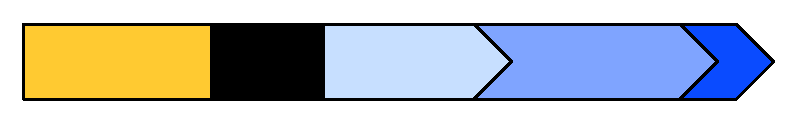
\includegraphics[scale=0.5]{figures/right-marking}  
%   \caption{A nested right-marking region, on the right of a carpet (black), and a border zone on its left.}
%   \label{fig:right-marking}
% \end{figure}

\item\label{i:outline.border-zone} 
It is also possible (even if seems less likely) that the head leaves the carpet
in normal mode.
This can happen in two ways: as part of zigging, when it makes no changes,
or advancing the front, and thus making changes on the tape.
In the first case, the healing interval will not be extended.
In the second case, we extend the island (since these changes may have
just been caused by the carpet) as in Definition~\ref{def:extending-islands}.
In both cases, as zigging brings back the head to attack the carpet,
an interval of unmarked cells may arise at the border of the healing
interval that is consistent with the area outside (could be united with it without
affecting health): it will be called a \df{right normal zone} below.

\item\label{i:outline.leaving-marking}
The head can leave a right marking zone or border zone only by hitting another carpet
or by possibility~\ref{i:outline.mop}.
% Therefore normally at most one carpet is surrounded by marking regions on both sides: the
% one containing the head.
% The other ones have a border zone on their side facing the head.

\item If a carpet disappears with a border zone on both sides, and no alarm
is called, then the healing interval can also be erased, as in Definition~\ref{def:shrinking}.

\item What happens when a right marked zone reaches another carpet on the right?
When the head returns from this other carpet, it may
extend a new left marked zone, or continue the work on the marked zone
that was already there.

\item After entering a marked zone or normal zone from a carpet, the head makes at most one turn
before hitting a carpet again.

\item Once a carpet disappears it may take more switches to hit a carpet again.
But every turn brings some progress: bringing closer to a carpet,
increasing the size of the marked region, or pulling away from all the carpets.

\item\label{i:outline.mop} If the head does no pull away then a 
healing procedure will be carried to the completion of its repair stage (by this time
any possible carpets in its way have been erased).

Now if the healing area on which the procedure worked is equal to a whole healing interval,
then the mopping stage will shrink it accordingly, as in Definition~\ref{def:shrinking}.
Otherwise, a new alarm will start at one of its ends; as we will see, this process
will still terminate in a few iterations.

\item As a complication, a burst can create a new carpet at any time of this history;
we will analyze its possible effects.

\end{enumerate}


\begin{definition}[Regular annotation]\label{def:regular-annotation}
In an annotated configuration, 
consider a clean interval \( I \) of cells marked for healing or rebuilding
(that could have been) created by the healing or rebuilding procedure.
Assume that if the head is on the left of \( I \) then the last healing or rebuilding
sweep was to the left, and the right end of \( I \) is either next to a carpet,
or is where the head turned back last time in the healing procedure.
Such an interval will be called a \df{right marking zone}.
Its \df{age} is the number of its current healing sweep.

Consider two adjacent intervals \( J,K \) such that
\( K \) is at the stage of a right mopping sweep of the healing procedure
(thus the front is to its right), further 
the interval \( J\cup K \) becomes healthy after taking away the healing or rebuilding
marks from \( K \).
We will call \( J\cup K \) \df{right pre-healthy}.

Consider a clean interval \( J \) with a nonempty healthy interval 
or interval \( K \) marked for healing or rebuilding, adjacent to \( J \) on the right.
We call \( J \) a \df{right border zone} if \( J\cup  K \) is healthy or right pre-healthy.

% Any right end segment of \( I \) will be called a \df{right marking region}.

An annotation is \df{regular} if every carpet to the right or under the head has a
right border zone or marked zone on its right.
Similarly on the left.

\end{definition}

% Here are some important properties of regular intervals:

% \begin{lemma}\label{lem:regular}
% If (in the absence of noise) the head enters a right-regular interval \( I \)
% from the left, then the following holds.
% \begin{alphenumIn}
%   \item  Alarm can only be called on the first cell.
% Whether it alarms or not, the head will either pass through \( I \) or return 
% from it on the left while leaving it right-regular.
%   \item\label{i:regular.mop-zig}
% If \( I \) contains a nonempty complete right-regular interval then
% the head cannot exit on the right, with one exception: 
% while performing the zigging part of the
% mopping stage of the healing procedure -- this requires the age of \( I \) to be
% maximal.
% \end{alphenumIn}
% \end{lemma}
% \begin{proof}
% In case of alarm, the head will start a new marking region on the left; otherwise
% it will continue the job of extending the existing innermost marking region,
% or if the nested marking region is empty, start moving in the border zone.
% In the latter case again, since it did not alarm on the first step it will have to
% accept the rest of the border zone as well.

% Part~\ref{i:regular.mop-zig} follows since there is no other way for the head
% to leave a marked area.
% \end{proof}

% \begin{definition}[Regular annotation]\label{def:regular-annotation}
% it has the following properties.
% They must hold also with the interchange of left and right.


% Consider a healing interval \( G \) not containing the head.

% \begin{alphenumIn}

%   \item
% If it has a nonempty carpet then it is an island.

% \item Its part to the right of the carpet (or of the point at which the carpet
% disappeared) is right-regular, and complete right-regular unless adjacent to a carpet on its
% right.

% \item\label{i:regular-annotation.entering}
% At a time when the head enters \( G \) from the left
% then \( G \) consists of three consecutive
% parts (each of which can be empty): a left border zone, a carpet, and
% a right-regular interval that is complete right-regular unless adjacent to a carpet on its right.

% % \item  % Do we need this?
% % If \( \abs{I}>\cns{isl-bd}\B \) then \( I \) consists of a single marking region.  
% \end{alphenumIn}
% \end{definition}

% Part~\ref{i:regular-annotation.entering} says, essentially,
% that the head cannot enter a left marking region of a healing interval \( G \)
% from the left without overwriting it by another healing interval that is 
% extending from the left.

% Let \( \sigma \) be the size of the union of these stains, \( \chi \) the size of the union of carpets 
% inside them.
% % , and \( \alpha \) the maximum age of any of the healing intervals.
% % Let \( m \) be the number of the last marking sweep of the healing procedure.
% Then \( \chi\le k\beta\B \) further
% \begin{align*}%\label{eq:annotated-config.island-bounds}
%       \sigma +\F \chi &\le k(\F+2)\beta\B.
% % \\    \alpha + \chi    &\le m + k\beta.
%  \end{align*}
% in particular \( \sigma\le k(\F+2)\beta\B \). 
%, \( \alpha\le m + k\beta \).

%
%        \item \label{i:annotated-config.ptr}
%          The \( \cDir \) field of each clean cell of \( A \) points towards the head.

%        \item
%          What I meant is that if the head is in the
%          annotated configuration then the annotated configuration must
%          contain the current colony
%          (base colony is OK, just make sure it is clear that it
%          corresponds to the current cell of M^{*}).

% The inequalities in~\ref{i:annotated-config.island-bounds} limit the amount 
% by which stains % and the age of healing intervals
% can grow.
% This depends on the presence of carpets.
% A carpet may send the head out, causing its island to grow.
% But every at most \( \F \) steps of extending the island
% will be followed by switchback: either due to zigging, or due to the gradual
% manner of the extension of the healing area.
% Re-entering and re-exiting a carpet will then shrink it.
% The formula shows just this: except possibly for the first time when exiting on each side,
% the growth of the islands is paid for by the decrease of the carpets.
% The upper bound arrived at deserves a notation: let
% \begin{align}\label{eq:isl-bd}
%    \cns{isl-bd} = (\F+2)\beta,
%  \end{align}
% then the total size of \( k \) stains is bounded by \( k\cdot\cns{isl-bd}\B \).
% We require the formula for a group of \( k \) stains for a minor technical reason,
% and the fact that we want to be able to do induction with it.
% It can happen that that two carpets \( I_{1}, I_{2} \) are adjacent.
% Now the head may enter \( I_{1} \) on the left, slide over to the right end of \( I_{2} \),
% extend its island somewhat, then return and leave again on the left end of \( I_{1} \).
% Now in order to balance the increase of the island of \( I_{2} \) on the right,
% we take into account the decrease of the carpet \( I_{1} \) on the left.

% \begin{lemma}\label{lem:new-burst} 
% Definition~\ref{def:carpets} extends the annotation to after the burst in a regular way.
% \end{lemma}
% \begin{proof}
% This is straightforward.
% \end{proof}

\begin{lemma}\label{lem:clearing} Suppose that a regular annotation has been defined
on an interval, starting from a healthy configuration,
using Definitions~\ref{def:carpets}, \ref{def:extending-islands} and~\ref{def:shrinking}
while the bursts are sparse, up to a time when distress occurred.
Then it extends until a time when either the the head becomes safe or it finds
itself in a fully extended, carpet-free healing area at the end of the marking stage.
\end{lemma}
From now on we will only consider regular annotations, without always mentioning
this explicitly.
\begin{Proof}
\begin{step+}{step:clearing.health}
Property~\ref{i:annotated-config.health} is conserved.
\end{step+}
\begin{prooof}
Indeed, for this property we only need to be concerned with deleted islands.
But by our definition we only delete islands when this can be done
without affecting the health of the underlying configuration.
\end{prooof} % step:clearing.health

\begin{step+}{step:clearing.island-number}
Property~\ref{i:annotated-config.island-number} is conserved.
\end{step+}
\begin{pproof}
Consider any interval of size \( Q\B \).
At time \( t_{0} \) it intersects at most 3 stains.
Our concern is to show that it cannot intersect more at time \( t_{1} \).
If there are only 2 such stains then there is nothing to prove, since
at most one more burst can occur between \( t_{0} \) and \( t_{1} \).
Let \( u_{1}<u_{2}<u_{3} \) be the three times at which the burst
causing the three stains \( I_{1},I_{2},I_{3} \) occurred, and 
let \( u_{4}>u_{3}\) be the time of the new burst.
By Property~\ref{i:annotated-hist.relief.one-dir} of annotated histories,
the next time the head approaches \( I_{1} \) at time \( u_{2} \),
it cannot pass through \( I_{1} \),
since this would mean a relief event without turn, and then
\( I_{1} \) would have been erased.
So it must make a turn within a work period after the time \( u_{2} \).
But then by the feathering property of the simulated cellular automaton \( M^{*} \),
by the time the head returns again, at time \( u_{3} \),
the simulation cannot make another turn.
Within a work period it must pass through \( I_{1} \) and \( I_{2} \)
and delete them.
So at most one stain could be left until time \( u_{4} \), 
the one coming from \( I_{3} \).
\Pnote{Closer estimation of distances needed here.}
\end{pproof} % step:clearing.island-number

\begin{step+}{step:clearing.regularity}
Regularity and property~\ref{i:annotated-config.island-bounds} of
an annotated configuration are conserved.
\end{step+}
\begin{pproof}
The history starts from a healthy configuration, so each stain starts as a carpet
of size \( \le 4\beta\B \).
The above definitions allow a stain to become bigger than the
island it contains only when the island is deleted.
Since the present proof only considers the growth process, not the deletions,
in talking about stains we will only talk about the islands.

To see the conservation of regularity consider a head leaving a carpet on the right.
It enters a right border zone or marking zone.
By the definition of these zones it will either continue all the way to another carpet,
or return at the end of the zone.
It is not possible to call alarm in the middle.
As a result, regularity is conserved.

For property~\ref{i:annotated-config.island-bounds} observe that an island can
only be extended into a non-marked area
by advancing a (seeming) front: this is followed by a zig within \( \F \) steps.
This necessarily hits the carpet in the island, since as the island started from a
carpet, this carpet cannot be too far back.

% Besides the conservation of regularity we will show that an island can grow only
% at the expense of the decrease of some carpet in it: a decrease of a carpet
% by one cell pays for the growth by at most \( \F \) cells.
% This will prove the upper bound \( \cns{isl-bd}\B \) with
% \( \cns{isl-bd} \) defined in~\eqref{eq:isl-bd}.
% The same argument bounds also the age of the healing interval.

% Suppose that the head arrives from the left at an island \( I \).
% By regularity, the part on the left of the leftmost carpet \( I' \) of \( I \) 
% is a left marking zone or left border zone.
% Hence no alarm will be called before the head reaches the carpet
% at some time \( t_{1} \).

% Consider a later time \( t_{2} \) when the head exits the carpet \( I' \).

% \begin{step+}{step:clearing.leave-left}
% Assume that the head exits on the left.
% (Due to shrinking, the left end of \( I'(t_{2}) \) 
% is at least a distance \( \B \) to the right of the left end of \( I'(t_{1}) \).)
% \end{step+}
% \begin{prooof}
% If the left neighbor cell of \( I' \)
% will be marked then it will be added to \( I(t_{1}) \) if it was not there.
% \Pnote{Rebuild mode?}
% From now on the head cannot leave the island \( I \) on the left
% before its carpet will be erased, unless it meets another carpet on the left.
% The same happens if the mode is normal but alarm will be called immediately.
% Property~\ref{i:annotated-config.island-bounds} is conserved since
% extensions of the island to the left are accompanied by a switchback
% every \( \le\F \) steps, causing the head to enter the carpet and to decrease it 
% on the next exit.

% Suppose that alarm will not be called.
% Then alarm will not be called later either before reaching another
% healing interval, since what is found will be compatible with health.

% If the head will not change the cell's sweep then it will not change anything
% else in the \( \cCore \) track either, and the left boundary of island \( I \) 
% will not be changed: this happens only while zigging.
% If the zigging is descending then the head either reaches another island or returns
% to \( I' \).
% If it is ascending then the head will move until it reaches the front: this is 
% necessarily outside \( I \) since in this case it must have been the zigging that
% reached \( I \) to begin with.

% If the head changes the cell's sweep then the situation is locally compatible
% with having a left-moving front at the head.
% The front will be moved left repeatedly, with the cells added to island \( I \)
% (if they were not there), until either reaching another healing interval or
% starting to zig right: all this keeps the area between the islands healthy.
% The configuration between the head and \( I' \) remains healthy.
% Property~\ref{i:annotated-config.island-bounds} is conserved since
% extensions of the island to the left are accompanied by a zigging switchback
% every \( \le\F \) steps, causing the head to enter the carpet and to decrease it 
% on the next exit.
% \end{prooof} % step:clearing.leave-left

% \begin{step+}{step:clearing.leave-right}
% Assume that the head leaves \( I' \) on the right.
% \end{step+}
% \begin{prooof}
% By the assumption that regularity holds until now, the right end of \( I \)
% outside \( I' \) is either a right nested marking region or a right border zone.

% In the first case when the head steps on it, it can only either call alarm and
% start a new innermost marking region, or continue
% extending the current innermost marking region.
% It can only exit on the left by entering the carpet \( I' \) again.
% It can exit this region on the right only by either reaching another carpet,
% or by the possibility~\ref{i:regular.mop-zig}.
% Property~\ref{i:annotated-config.island-bounds} is conserved just as above.

% In the second case, if the head calls alarm then it is starting a right marking
% region, and from here the above reasoning applies.
% Otherwise it is moving the front right or zigging.
% If it is moving the front then the cells it passes before returning in a zig 
% are added to the island \( I \) (if they did not yet belong to it); no alarm will be called.

% If it is zigging then, 
% since the border zone is part of a healthy area, the zigging can proceed 
% without alarm.
% If it is ascending then it ascends until reaching the front or another carpet.
% If it is descending then
% it either encounters another carpet or reaches the maximum depth.
% In the latter case the head will return to \( I' \) without alarm.

% Property~\ref{i:annotated-config.island-bounds} is conserved just as above.
% \end{prooof}% step:clearing.leave-right

\end{pproof} % step:clearing.regularity

Now consider the stages of the development of the healing intervals between
times when the head is in a carpet.
By regularity, after a head leaves a carpet \( I \) and assuming this carpet is still not empty,
the head will either hit another carpet within a single sweep or return to \( I \) within
a pair of sweeps, of a total length \( \le 2\E\B \) (the maximum length of a healing area).
After each such event, some carpet decreases.
If a carpet disappears then the head, provided it did not become free,
either starts a progress (with zigs) in some direction
or starts extending a healing area (it may start with the first and continue with the second).
It cannot extend a rebuilding area: indeed, on trying this, zigging would check whether there is a
large enough interval marked for rebuilding which to extend further.
If the head does not hit a carpet then it will find out that there is not such an interval, and
will call alarm.

Certainly in at most \( 4\E \) sweeps, it will either hit another carpet, or become free,
or extend a carpet-free healing area to its maximum size.
Since there are at most 3 carpets to consider, the process terminates soon.

The possibility of a burst during this history does not change the reasoning, since it just
creates a new carpet without destroying regularity.
\end{Proof}

% As the above analysis shows, if a cell \( x \) gets marked for healing just as the head
% steps off an island \( I \) then \( x \) will be added to \( I \).
% This limits the healing interval of \( I \) to \( I \) itself, and hence also its
% size by~\ref{i:annotated-config.island-bounds}.
% Once its carpet disappears, however, a healing interval can increase further --
% but at least its structure simplifies soon:

% \begin{lemma}\label{lem:non-island}
% In the annotation of Lemma~\ref{lem:clearing}, once a healing interval \( I \)
% loses its carpet then it becomes a marking region before
% its size (and age) reaches \( 2\cns{isl-bd}\B \).
% \end{lemma}
% \begin{proof}
% At the time when \( I \) loses its carpet it is an island consisting of a 
% right-regular and a left-regular part, separated by the head.
% Now it starts (or continues extending) a marking region which will cover \( I \)
% before it doubles its size -- unless it hits another carpet earlier, which can
% stop its growth on that side.
% \Pnote{Recompute.}
% \end{proof}

Let us limit the size and age of intervals not containing the front.

\begin{definition}\label{def:mainland}
The healing interval containing the front will be called the \df{mainland} (it could be empty).
\end{definition}

\begin{lemma}\label{lem:mainland}
Consider the annotation of Lemma~\ref{lem:clearing}.
In any interval \( A \) of
size \( Q\B \), the total size of the non-mainland healing area
is \( <17\Z\B \), and its age is bounded by \( 9\Z \).
\end{lemma}
\begin{Proof}
In what follows we only consider events and parts of the tape
in the interval \( A \), without pointing this out repeatedly.

\begin{step+}{step:off-mainland.distance}
If two consecutive healing intervals are not adjacent then the 
distance of their carpets is \( \le 2\Z\B \).
The same bound applies to the healing area's distance from the front.
\end{step+}
\begin{pproof} 
Only a jump can bring the head from the front (if it is outside
the healing area) to a healing area, or from a healing interval to a
non-adjacent other one.

A downward jump is produced by the descending part of zigging, so it 
makes at most \( \Z \) steps.
An upward jump can only happen after a downward jump; indeed, 
it is going towards the front, from whose healing interval
the head first had to get away by downward jumps.
\end{pproof} % step:mainland.distance

\begin{step+}{step:off-mainland.size}
Let us estimate the total size of the off-mainland healing area.
\end{step+}
\begin{prooof}
Consider the first time when the carpet of some healing 
interval disappears.
Just as we bounded the size of islands, we can bound the size of the total healing area
at this time as \( 3\cns{isl-bd}\B \).
In what follows we ignore this quantity, since \( \Z \) will be chosen
bigger than \( 3\cns{isl-bd} \).
At the end, we will correct for it.

Once a healing interval starts to grow after losing a carpet, it does
so by the marking stage of the healing procedure, therefore grows symmetrically.
If it starts at a distance \( x \) from the front then it can only grow to a
size \( 2 x \) before merging with the mainland.
Distance \( x \) could have reached only either by a jump, or by the growth
or another healing interval closer to the front.
It is easy to see that the second possibility takes at least as far 
in the extreme cases.
So if \( x_{1},x_{2},x_{3} \) are the starting points of the healing intervals
seen from the front then the farthest we can get is essentially
\( x_{1}=2\Z\B \), \( x_{2}=4\Z\B \), \( x_{3}=8\Z\B \).
This gives a bound of \( 16\Z\B \) on the total size of the the off-mainland healing
area: we add \( \Z\B \) to correct for ignoring the bound
\( 3\cns{isl-bd}\B \) on the total size of the islands.
\end{prooof} % step:mainland.size

\begin{step+}{step:off-mainland.age}
The estimate of the age of the off-mainland healing area is similar.
\end{step+}
\begin{prooof}
Indeed, almost each age increase is associated with a sweep in the marking stage
and hence the addition of a cell to some healing interval.
The exception is only when the sweep hits a carpet, but as these events
decrease the carpets, they can happen only \( 3\beta \) times.
We bounded the total area essentially by \( 8\Z \) cells, which gives a bound
of \( 8\Z \).
With the corrections due to carpets we are still within \( 9\Z \).
\end{prooof} % step:mainland.age

\end{Proof} % lem:mainland

Given that the healing area off the mainland remains young,
the healing procedure only gets a chance to work on the mainland.


% Let us summarize what we learned about the annotation, as it gets extended.
% \begin{itemize}
% \item 
% Each healing interval is left-regular to the left of the carpet (or a point where the
% carpet disappeared), and right-regular to its right.

% If the head enters it then it will continue extending in a regular way on both sides of
% its carpet, as long it has a carpet; it becomes regular within a sweep 
% after that.

% \item
% The part of the healing area that is not the mainland remains small and young.

% \item The mainland, if it exists, keeps maturing its healing intervals,
% and does not break up.
% If a new burst occurs (which can only happen once), it creates a new carpet 
% (equal to its own new healing interval), 
% possibly cutting an existing healing interval into two.
% \end{itemize}

\subsection{Relief}

After these preparations, we are ready to prove that (small) distress is always followed
by relief.

\begin{definition}[Ready healing intervals] 
An interval of the mainland is \df{ready} if it is clean, consists of cells marked for
healing with consecutive healing addresses, extended to the maximum size by the
healing procedure, its age is still within the marking stage, and contains the
head in a state allowing it to continue the healing procedure.
\end{definition}

\begin{lemma}[Relief]\label{lem:relief} Suppose that a regular annotation has been defined
on an interval, starting from a healthy configuration,
using Definitions~\ref{def:carpets}, \ref{def:extending-islands} and~\ref{def:shrinking}
while the bursts are sparse, up to a time when distress occurred.
Then it extends until a time when either the the head becomes safe: in other words, the distress
is followed by relief.
\end{lemma}
\begin{proof}
% \begin{lemma}\label{lem:ready}
% Under the conditions of Lemma~\ref{lem:clearing}, a time comes 
% \Pnote{Bound?} when
% either the head becomes safe (per Definition~\ref{def:safe}), 
% or it is in a ready healing interval in the mainland.
% \end{lemma}

% \begin{Proof}
% Given the bound on age of the non-mainland part of the healing area \( \H \), 
% if there is no mainland then the head cannot spend much time
% in \( \H \) before leaving it and becoming safe.
% Suppose therefore that there is a mainland.
% Only hitting a carpet (or a new burst) can stop the extension of 
% a healing interval of the mainland.
% But this can only delay the growth along with its 
% aging: sooner or later one of these intervals will become ready.
% \end{Proof}

By Lemma~\ref{lem:clearing} sooner or later the annotation gets extended
to a stage in which the head is either free or is in a ready interval of the healing area.
Let us summarize what follows after this, first ignoring the possibility of a new burst.
\begin{description}
\item[Repair] 
Working on a ready interval \( R \), the head carries out
the rest of the healing procedure of Section~\ref{sec:healing-proc}, 
\emph{provided} no burst occurs.
It will change islands and compute the position of the front, exactly
if it is inside \( R' \), or just the direction from \( R' \) if it is outside.
Then it will start the mopping part, say, on the left (definitely on the left if
the front is to the right of \( R' \)).

\item[Left shifts] If the zigging part of mopping finds no marked cell
then the mainland ends on the left.
Indeed, the unmarked cells belonging to a healing interval must have belonged
to islands before, so their total number is bounded by a bound on the total size
of islands.

If it finds some marked cell, it calls alarm, and thus restarts
the process, which can end only with a ready
healing interval \( G \) shifted by about \( \E \) cells to the left of \( R \).
It may be shifted more, if a carpet captures the head causing it to develop
another healing interval to the left of \( G \),
but not less, since there is no carpet in \( R \) anymore.
This restart may be repeated, but again only by shifting to the left:
indeed, the mopping always starts at the side away from the front.
This way, eventually the left end will get repaired and mopped clean.

\item[Right shifts] Now an alarm on the right end (called either because
the front is to the right or because the mopping zig discovered a marked cell)
restarts the process on an interval shifted about \( \E \) cells to the right.
This right shift can also be repeated several times.
Eventually the right end will also be repaired.

\item[Final left shifts]
The repaired right end could also be away from the front, in which case
again some left shifts will bring back the repair process to the front.
\end{description}

The case that still needs to be examined is when a burst occurs
during the healing procedure.
Let \( K \) be the new carpet (possibly united to some existing carpet),
and let us call it \( K(t) \) at later times \( t \).
If at any time after this, alarm is called on exiting \( K(t) \)  in such
a way that the healing procedure cannot conclude,
then the reasoning of Lemma~\ref{lem:clearing} can be repeated,
and now the process concludes without further interruptions. 

Suppose now that no alarm prevents the healing process on \( R \)
from concluding.
Then the changes in the healing process will be confined to the area of the
carpet \( K \) and possibly \( \beta \) more cells neighboring it.
Indeed, the construction of the Repair stage of the healing procedure
does not allow any repair changes that were not decided also in an earlier
decision.
One of the two decisions will be taken over a clean healing area \( R \).
If they do not coincide then the changes will not take place anywhere but
over the carpet \( K \) itself, and possibly \( \beta \) cells if the carpet
initiates a false stitching operation.

Due to the construction of the mopping process also,
if no alarm is called then the changes caused by the burst
during it are confined to the carpet \( K \).
\end{proof}


\section{After a large burst}

Our goal is to show that the simulation \( M\to M^{*} \)
defined in Section~\ref{sec:sim-codes} is indeed a simulation.
Section~\ref{sec:1-level-noise} shows this as long as the head operates in an
area that is clean for the simulated machine\( M^{*} \) (can be super-annotated), 
and has no noise for machine \( M^{*} \) (that is its bursts on the level of machine \( M \)
are isolated).
In other words, essentially the Transition Function property of Definition~\ref{def:traj} of
trajectories for the simulated machine \( M^{*} \) has been taken care of.

The new element is the possibility of large areas that cannot be super-annotated: they
may not even be clean, even on the level of machine \( M \).
The Spill Bound, Attack Cleaning, Dwell Cleaning and Pass Cleaning properties still must be proven.

\subsection{Spill bound}

One of the most complex analyses of this work is the proof that 
the simulated machine \( M^{*} \) also obeys the Spill Bound.
Let us outline the problem.

We are looking at the boundary \( z \) of a large area that is clean for the
machine \( M^{*} \): without loss of generality suppose that this is the right boundary.
We will be looking at it in a space-time rectangle \( \lint{a}{b}\times\lint{u}{v} \)
that is noise-free in \( M^{*} \).
The interesting case has \( a<z<b \) with \( z-a=b-z=O(Q\B) \).
The assumption allows occasional bursts of noise of the trajectory \( \eta \) of \( M \),
but no two of these bursts must occur in a space-time rectangle of size comparable to
the size of a colony work period of \( M \).
The Spill Bound for trajectory \( \eta \) keeps the dirt of \( \eta \) within
\( O(\B) \) on the left of \( z \) while \( \eta \) is noise-free.
If we could assume \( \eta \) noise-free then the heal/rebuild procedures would also keep
the dirt of \( \eta^{*} \) from spilling over by more than \( O(\B^{*})=O(Q\B) \).
However, nothing is assumed about the length of the time interval \( \lint{u}{v} \).
If the head would spend all the time within \( O(Q\B) \) of \( z \) then due to 
the Dwell Cleaning property of trajectories,  the area would be cleaned out, again
preventing spilling.
But the head can slide out far to the right of \( b \) fast, since
the dirty area on the right of \( z \) is arbitrarily large.
Then it can come back much later to the left of \( z \), and by
a burst (allowed since much time has passed)
can deposit an island of dirt there.
Repeating this process would produce unlimited spillover, not only 
of the dirt of \( \eta^{*} \) but even that of \( \eta \).

This is where the Pass Cleaning property helps.
If the above process is repeated \( \pi \) times, the \( \pi \) passes
would clean out an interval on the
right of \( z \) whose size is of the order of \( Q\B \),
while depositing only \( \pi \) islands of dirt to the left of \( z \).
Our construction will have \( \pi\ll Q \): more precisely, in our hierarchy
of generalized Turing machines we will have \( \pi_{k}=k \), \( Q_{k}=k^{2} \). %?
And \( \ll Q \) bursts will still be handled by healing/rebuilding in \( \eta \).

Of course this sketch is very crude, but it should help motivate the reasoning that
follows.



\bibliographystyle{plain}
\bibliography{reli,publ}

\end{document}
%%% Local Variables: 
%%% mode: latex
%%% TeX-master: t
%%% End: 
